\documentclass[preprint]{aastex}

\usepackage[top=1in, bottom=1in, left=1in, right=1in]{geometry}
\usepackage{amsmath}
\usepackage{graphicx}
%\usepackage{mdwlist}
\usepackage{natbib}
\usepackage{natbibspacing}
\usepackage{enumitem}
%\usepackage{caption}
%\usepackage{subcaption}
\usepackage{float}
\setlength{\bibspacing}{0pt}
\setlength{\parskip}{0pt}
\setlength{\parsep}{0pt}
\setlength{\headsep}{0pt}
\setlength{\topskip}{0pt}
\setlength{\topmargin}{0pt}
\setlength{\topsep}{0pt}
\setlength{\partopsep}{0pt}
\setlength{\footnotesep}{8pt}
\pagestyle{empty}
\citestyle{aa}
%\usepackage[font=small]{caption}


\newcommand{\compress}{\vspace{-0.12in}}


\def\kperp{k_{\bot}}
\def\kpar{k_{\|}}
\def\nwnh{{\sl NWNH}}

\newcommand{\simgt}{\stackrel{>}{_{\sim}}}
\def\kperp{k_{\bot}}
\def\kpar{k_{\|}}
\def\k{{\bf k}}
\def\sky{{\theta}}
\def\HI{{H{\small I }}}
\def\HII{{H{\small II }}}
\def\xHI{{x_{\rm\HI}}}

%project description 20 pages total

\begin{document}

%\title{Hydrogen Epoch of Reionization Array: Characterizing Cosmic Dawn}
\title{HERA: Illuminating Our Early Universe}
{\it For the Mid-Scale Science Projects category of the Mid-Scale
Innovations Program}

\begin{figure}[H]\centering
\includegraphics[width=6in]{plots/hera_array.png}
\caption{The proposed array of 331 14~m-diameter zenith-pointing dishes in the Karoo Radio Astronomy Reserve
in the Northern Cape of South Africa.
}\label{fig:hera_array} \end{figure}

% Parsons, Carilli
% A statement of which of the four categories of MSIP is most appropriate
%for this proposal as the first sentence (see section II. Program Description).
%A. We propose HERA: next step in reionization roadmap
%B. Fulfill NWNH high-priority goals
%C. New understanding/techniques => faster, better, cheaper
%D. Brief summary of timeline: science along the way, major results before end-decade

\vspace{-0.4in}
\section{Overview of this Proposal} % 1 page ~ project summary? 

% XXX
% I would really start out saying that this is a proposal to detect the EOR 21 cm
% at high enough significance to exclude models based on scale and redshift
% dependence of the power spectrum, plus map the brightest features.  The array
% itself is a consequence, not the driver, of the proposal.

The Hydrogen Epoch of Reionization Arrays (HERA) roadmap is a staged
plan for using the unique properties of the 21~cm line from neutral
hydrogen to probe our cosmic dawn, from the birth of the first 
stars and black holes, through the full reionization of the primordial
intergalactic medium (IGM). 
During these epochs, roughly 0.3--1~Gyr after the Big Bang, the
first stars and black holes heat and reionize the neutral
IGM that pervades the Universe following cosmic
recombination. Direct observation of the large scale structure of the primordial
IGM, and its evolution with time, via the \HI 21~cm line, will
have a profound impact on our understanding of the birth of the first
galaxies and black holes, their influence on the surrounding gas,
and cosmology. 

HERA was ranked the ``{\it top priority in the Radio, Millimeter, and
Sub-millimeter category of recommended new facilities for mid-scale
funding}" as part of the {\it New Worlds, New Horizons of Astronomy
and Astrophysics} decadal survey (\citealt{astro2010}; hereafter
NWNH).  The HERA roadmap initially envisioned a series of radio
interferometers constructed throughout the decade. Phase I of this roadmap
incorporated existing instruments --- the Donald C. Backer Precision Array to Probe the Epoch of
Reionization (PAPER) and the Murchison Widefield Array (MWA) ---
aimed at characterizing foregrounds and laying the
% ARP: I like "laying the graundwork" as a bit of a backstep from requiring a detection
groundwork for a statistical detection of the HI 21~cm signal through
the power spectrum.  A second-generation HERA instrument would measure
the evolution of the power spectrum to reveal details of the astrophysics
involved in the birth and evolution of galaxies 
in the early Universe. A third-generation instrument would
directly image structures throughout reionization.

% XXX do we want the "fraction of the funding" line?  ARP: I think it's ok as stands.
With a fraction of the funding recommended for HERA Phase I
in NWNH, the MWA and PAPER projects have made
major strides in developing techniques to disentangle
the reionization signal from the strong radio continuum foreground
emission.  These techniques, which are based on a new
understanding of the interplay of foreground and instrumental systematics
in the context of a three-dimensional cosmological intensity-mapping experiment,
have yielded a critical breakthrough.  As discussed below, {\bf we are now able to remove 
foregrounds to the limits of our sensitivity with these instruments},
and this is culminating in the first physically meaningful upper limits
on the power spectrum of 21~cm emission from reionization \citep{parsons_et_al2013}.

Current generation 21~cm reionization experiments (LOFAR, MWA, PAPER) are fully constructed and have been engaged in observations
that will soon reach the sensitivity limits of these instruments.  Meanwhile,
the principles that have yielded this breakthrough in foreground removal
have given us new insight into how
21~cm reionization experiments should be designed.  Based on these insights, we have developed a new 14~m diameter antenna element 
that is optimized both for
sensitivity and for minimizing foreground systematics.  
Arranging these elements in a compact hexagonal grid yields an array that
facilitates calibration, leverages proven foreground removal techniques, and is scalable
to large collecting areas.
%We place these elements on a hexagonal grid that is maximally compact,
%and minimize the length of the analog signal path, 
%producing a scalable design that can deliver
%levels of sensitivity and foreground removal that are transformative for
%the studying reionization.  
An instrument based on this design has the sensitivity to transform the field of 21~cm reionization,
going well past the first detection of the cosmological signal to the detailed characterization of 
its power spectrum, constraining reionization parameters at the $\sim$10\% level \citep{pober_et_al2014}.

With this scalable design, we are now ready to build the instrument
that delivers HERA-II science
a cost that is substantially below what was originally envisioned in NWNH.
We propose a four-year plan to conduct the next generation HERA experiment,
observing in the 50--225~MHz band, in two stages:
\begin{itemize}[noitemsep,nolistsep]

\item HERA~127, deployed at the end of the second year of this proposal, will measure the rise and fall of the 
21~cm reionization power spectrum, constraining the timing and duration of reionization.

\item HERA~331, deployed at the end of the third year, will measure fluctuations in the 21~cm
signal over a variety of spatial
scales to determine the nature and distribution of the first galaxies
that dominate cosmic reionization. HERA~331 will also extend precision
power-spectrum observations back to the end of the 'Dark Ages' ($z \sim 20$), 
when the first stars and black holes warm the primordial IGM. 
% ARP: these designs already said below
%Ultimately, HERA-331 will have the sensitivity to
%image directly the largest scale structures in the IGM during reionization.
\end{itemize}
Drawing on the heritage of PAPER and the MWA, the proposed program incrementally builds a 
sequence of dedicated experiments
optimized to fulfill the NWNH goal of characterizing the evolution of
the HI 21~cm power spectrum during cosmic reionization. In
its final stages, HERA may be capable of imaging the primordial
IGM --- a task previously only considered for third-generation
instruments. 

% XXX as above, emphasize the proposal is for the 21cm science; array is a consequence
This proposal is intended to be a self-contained package
supporting the core activities required for delivering HERA-II science,
including telescope development, construction, observing, data analysis,
and scientific products for each stage of the project.  As described
in the Project Management Plan, this approach minimizes
risks associated with external funding contingencies, but leaves room for
collaborators to leverage outside resources for augmenting the science
output of HERA in meaningful ways.

% XXX document map here?

%  ___     _                 
% / __| __(_)___ _ _  __ ___ 
% \__ \/ _| / -_) ' \/ _/ -_)
% |___/\__|_\___|_||_\__\___|

\section{Scientific Justification and Intellectual Merit} %total = 8 pages

\subsection{Introduction}    % 1 page + 1 fig = simulated Tb cube + PS evolution
% Furlanetto, Carilli

%i.physical concepts: reionization and dark ages
%ii. Current knowledge: various constrai	nts, 1st galaxy studies...
%iii. Important role of 21~cm studies highlighted in NWNH
%a. Typical ideal sim results: T_B vs. z 'cube' and corresponding power spectrum evolution (Fig)
%b. introduce some of the important parameters/processes explored: when? how? bubble scale? sources? inside out? [much of this could be left for below?)
%c. reemphasize that current knowledge is nil, yet demand is high
%d. emphasize unique (only?) probe of dark ages

The {\it cosmic dawn}, the period beginning with the birth of the first stars and culminating with the full
reionization of the IGM some 500 Myrs later, represents one of the last unexplored phases in 
the history of structure formation. During this period, a wealth of astrophysical and cosmological phenomena are at 
work. The characteristics of the IGM depend on the cosmic density field, the formation sites of the 
first luminous sources (e.g., their typical masses and clustering), their constituents (e.g., exotic Population III 
stars, more normal stars, stellar remnants, or supermassive black holes) their ultraviolet luminosities (which affect 
the IGM's ionization state), the efficiency and abundance of X-ray sources (which affect the IGM temperature), and 
even more exotic effects like the relative velocity of baryons and dark matter.  Exploring these early structures and their 
effects on each other and their environments was one of the top three ``{\it priority science objectives chosen by 
the [NWNH] survey committee for the decade 2012-2021.}"

%SF: This next paragraph worries me a bit because most of these probes have one or several competing groups working 
%on them, and if we get a referee from one of the groups we don't reference they might get pissy...right now 
%I've tried to be fair but terse here
Observations are now just beginning to penetrate into this early epoch, primarily at its tail end.  Recent 
measurements from the {\it Hubble Space Telescope} have pinned down the bright end of the galaxy luminosity function 
at $z \la 8$ \citep{bouwens_et_al2010, schenker_et_al2013} and begun to detect a few sources at even greater 
distances \citep{ellis_et_al2013, oesch_et_al2013}.  Meanwhile, a number of indirect probes have placed constraints -- 
albeit model-dependent ones -- on cosmic reionization, as summarized in the left-hand panel of 
Figure~\ref{fig:x_i_vs_z}. These include observations of resonant scattering of Ly$\alpha$ by the neutral IGM toward
distant quasars (the 'Gunn-Peterson' effect) \citep{fan_et_al2006}, the demographics of Ly$\alpha$ emitting 
galaxies \citep{schenker_et_al2012, treu_et_al2013,Faisst_et_al2014}, and Ly$\alpha$ absorption near the most distant quasar 
\citep{bolton_et_al2011}, as well as measurements of CMB temperature fluctuations \citep{planck_et_al2013}, 
polarization anisotropies \citep{page_et_al2007}, and secondary temperature fluctuations generated by the 
kinetic Sunyaev-Zel'dovich effect \citep{zahn_et_al2012_trunc, mesinger_et_al2012}.  Reionization models can be 
built from galaxy observations.  Recent examples suggest that the IGM may have been substantially neutral even at 
$z \sim 7$--8 (as high as $F_{HI} \sim 0.5$), with a tail of finite ionization ($\sim 0.1$) extending to high 
redshift ($z \sim 15$), driven by very early galaxy formation \citep{robertson_2013}.  The extrapolation to 
$z>8$ is particularly uncertain, as only a handful of candidate galaxies have been found during that earlier 
era (c.f. \citealt{oesch_et_al2013}).  Unfortunately, these important methods have limited reach: strong assumptions 
are required about the stellar populations and escape fraction of UV photons from the galaxies, while astrophysical 
constraints on reionization are highly model-dependent and the CMB provides only an integral measure of the process. 
Moreover, many of these indirect observations are in tension with one another, underscoring both the difficulty in 
their interpretation and the complexity of the reionization process.

The 21~cm ``spin-flip" transition of  neutral hydrogen has been recognized as potentially the most powerful probe 
of cosmic reionization and  the dark ages \citep{morales_wyithe2010, furlanetto_et_al2006}, as emphasized in NWNH: 
``{\it 
%SF: Is this quote from the RMS panel?  If so, does it appear in the final report?
The panel concluded that  to explore the discovery area of the epoch of reionization, it is most important to 
develop new capabilities to observe redshifted 21~cm \HI emission, building on the legacy of current projects and 
increasing sensitivity and spatial resolution to characterize the topology of the gas at reionization.}"  Because 
the Universe is almost entirely neutral before reionization, the HI 21~cm line provides a direct method to image 
the evolution of the primordial IGM, opening a unique window into the complex astrophysical interplay between the 
first luminous structures and their surroundings. Moreover, because of the cosmological redshift, we can associate 
the signal at each observed frequency with a particular emission time (or distance) and reconstruct a complete 
three-dimensional picture of the time evolution of large scale structure during this `last frontier' in 
observational cosmology. 
%SF: Personally I feel like the following is an exaggeration that could rub some people the wrong way!
The direct observation of the primordial IGM via the HI 21~cm line would be an achievement comparable in importance 
to the detection of anisotropies in the CMB.

\begin{figure}[!ht]\centering
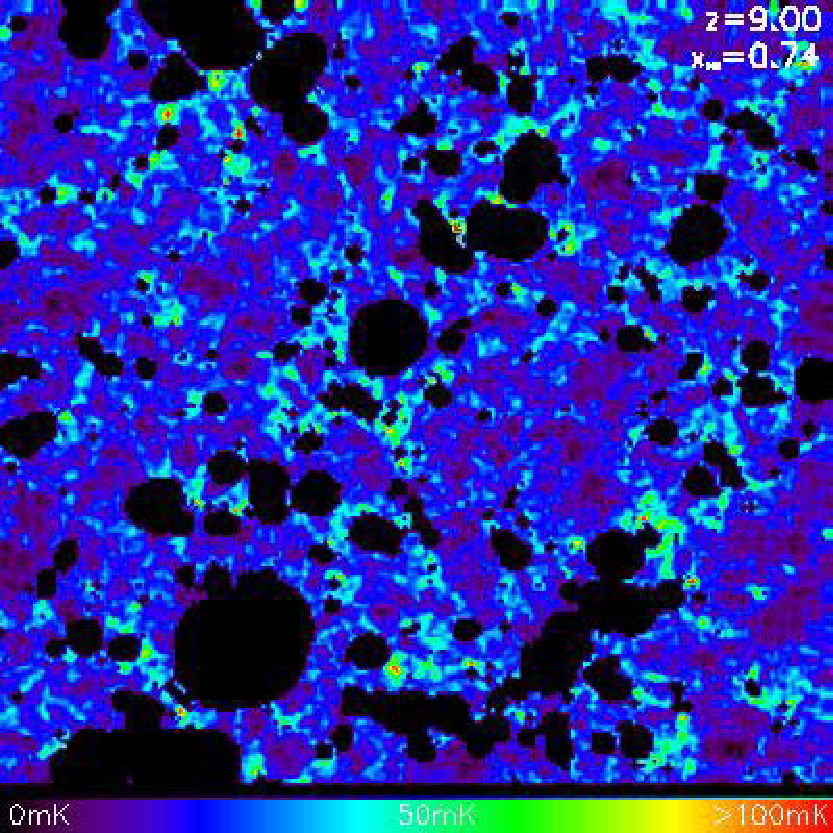
\includegraphics[width=0.23\textwidth]{plots/Pspec/z9sim.pdf}
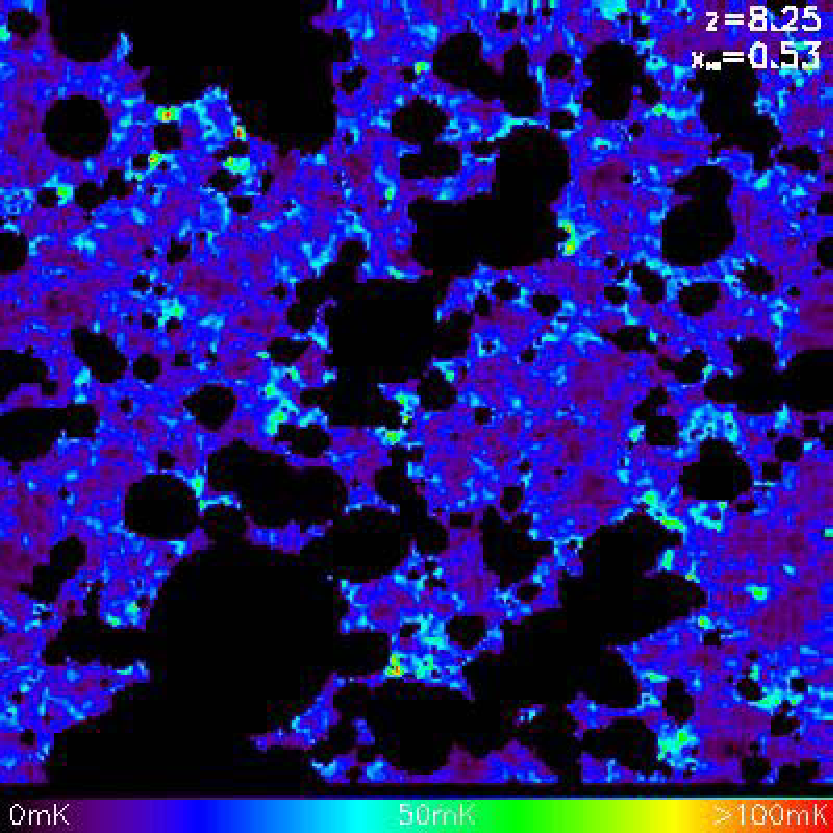
\includegraphics[width=0.23\textwidth]{plots/Pspec/z8sim.pdf}
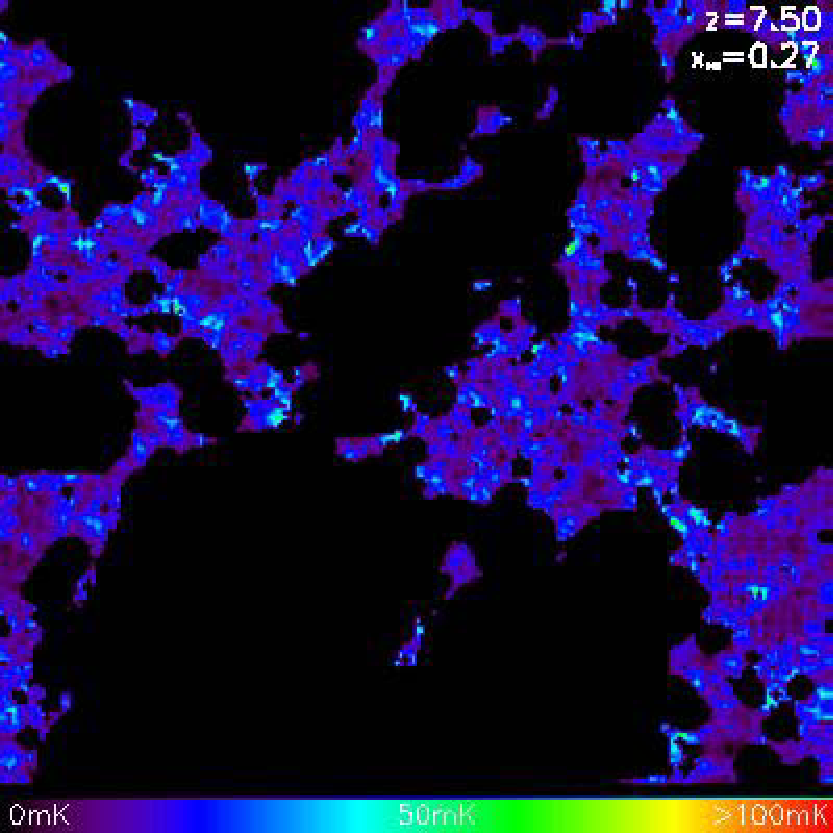
\includegraphics[width=0.23\textwidth]{plots/Pspec/z75sim.pdf}
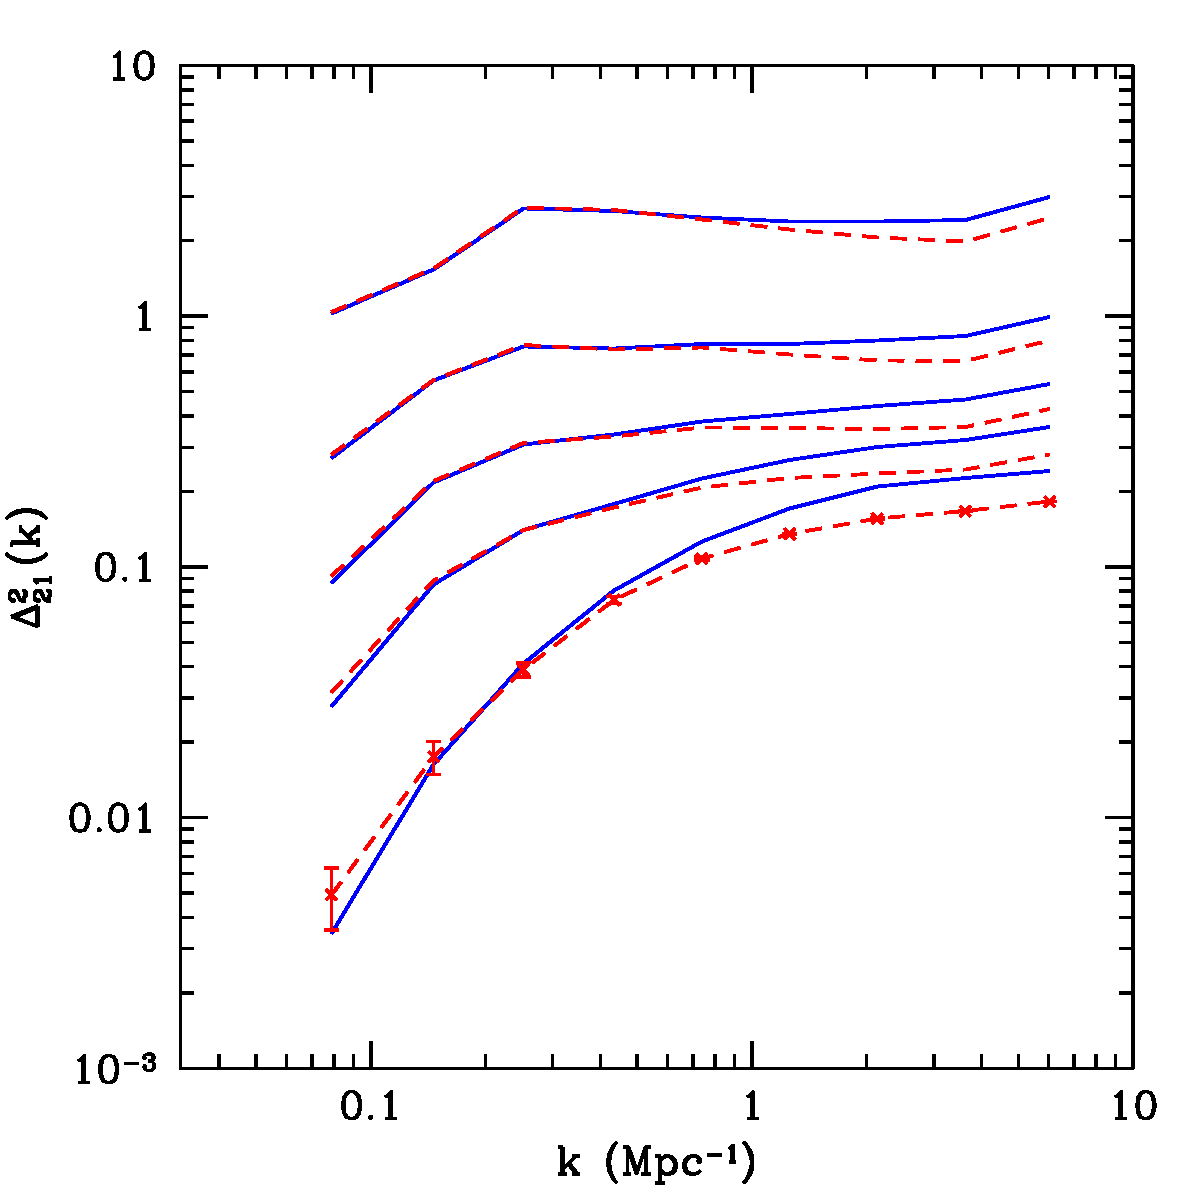
\includegraphics[width=0.23\textwidth]{plots/Pspec/pspecEvolve.pdf}
\caption{\small 
First three panels from left: simulated $21\,\textrm{cm}$ brightness temperature distributions at $z=9$, $8$, and $7.5$.  Rightmost panel: Evolution of the $21\,\textrm{cm}$ power spectrum from $z=9.25$ to $z=7$.  HERA will characterize the power spectrum in detail (Section \ref{sec:detectPspec}) as well as provide images of the ionized bubbles (Section \ref{sec:imaging_HI}).
}\label{fig:EoRsims} \end{figure}

In the past decades, considerable effort has gone into modeling the complex astrophysics of reionization
(e.g. \citealt{shapiro_giroux1987, haiman_loeb1997, furlanetto_et_al2004, santos_et_al2010}). Figure \ref{fig:EoRsims} shows a 
simulation of the expected evolution of the HI 21~cm signal during reionization \citep{mesinger_furlanetto2007}. The HI 21~cm fluctuations initially 
rise above those expected from the cosmic density field due to the growth of ionized bubbles on a characteristic 
scale of a few to 10~arcmin. This scale is set by the clustering of early galaxy formation, as well as by 
propagation effects through the IGM. The signal then declines as the IGM becomes fully ionized.  These theoretical 
models of the reionization process are sophisticated and appear to be well-understood, {\it but they are not 
predictive tools.} Instead, they provide a mapping between the largely unknown galaxy populations and observables 
like the 21~cm transition. As such, the key questions about the cosmic dawn era remain poorly understood.  When 
did reionization occur, and over what timescale?  What objects dominated the radiation field?  How were the 
objects distributed?  What were the most important feedback mechanisms in the transition from the first stars to
first galaxies, and how did they affect these populations?  {\it HERA provides the key measurements that are needed 
to advance our understanding of early galaxy formation and cosmic reionization.}


%Figures: F(HI) vs z;  HI Tb cube + PS evolution


\subsection{HI reionization and dark ages science} % 4 pages total examples using hera 331, plus a number of figures

\begin{figure}[t]\centering
%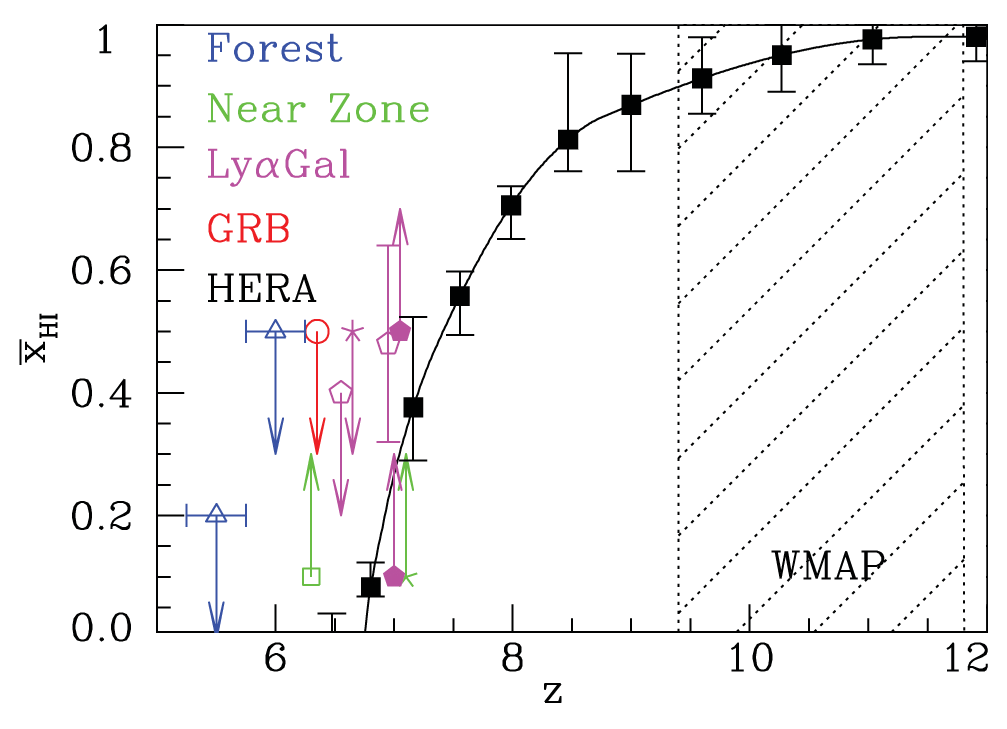
\includegraphics[height=2.25in]{plots/constraints_crop.pdf} 
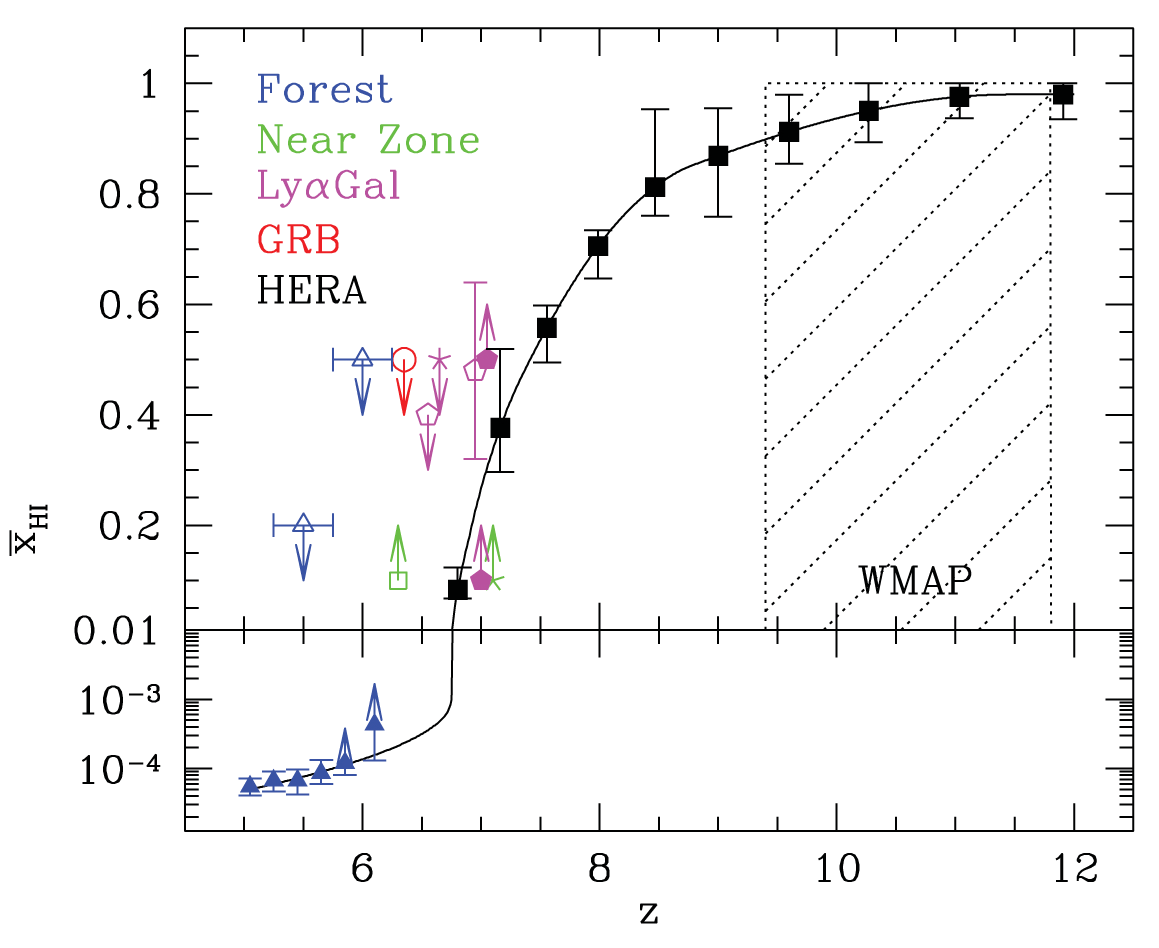
\includegraphics[height=2.25in]{plots/constraints.pdf}
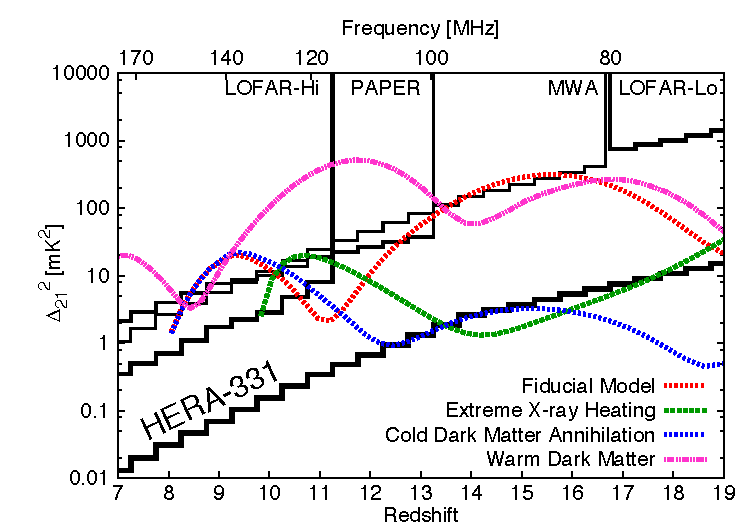
\includegraphics[height=2.25in]{plots/Xray/HERA_II_compare_kp1_whoriz_20pt.pdf} 
\caption{\small 
Left: 
Adapted from \citet{robertson_2013}, this figure shows existing
constraints (colored symbols) on neutral fraction, $\xHI$, versus redshift, along with 
the constraints HERA would provide (black markers, assuming
that $\xHI$ decreases versus redshift) for a fiducial
reionization history (black line).
At redshifts 8--12
21~cm emission may be the only precise probe of $\xHI$.
Right: At low frequencies, HERA probes
pre-reionization physics at the end of the Dark Ages. Plotted are power spectrum amplitudes (at $k =
0.15h$~Mpc$^{-1}$) for various IGM heating models \citep{mesinger_et_al2013},
with predicted sensitivities.
}\label{fig:x_i_vs_z} \end{figure}

As a high-sensitivity instrument with broad frequency coverage, HERA can
paint an uninterrupted picture through reionization, back to the end of 
the Dark Ages. This capability leverages the coupling of
21~cm emission to the properties of the first galaxies that
are inaccessible through other means,  and will be transformative for
studying the imprint of the very first galaxies in the Ly-$\alpha$ and X-ray backgrounds.  

Figure~\ref{fig:x_i_vs_z} illustrates how HERA will
reach beyond the late stages of reionization to measure the
ionization of the IGM throughout reionization, definitively constraining the timing
and duration of reionization.  At earlier epochs ($z \sim 15$ to 20), the sensitivity of the 21~cm line 
to the IGM temperature provides a unique probe of processes that warm the neutral IGM at the
end of the dark ages (see section XXX on dark ages).  HERA will have the low frequency coverage and
sensitivity to study these earliest phases of star and black hole formation -- an epoch that may be otherwise
untestable using other techniques.

Overall, as illustrated in Figure \ref{fig:x_i_vs_z}, observing 21~cm emission from the IGM with HERA 
promises to determine the ionization history of our universe much more precisely,
and at higher neutral fractions (wider redshift range), than is possible with other existing techniques.  These measurements can
be used to move beyond characterizing the timing and duration of reionization to
explore which galaxies dominate the integrated UV luminosity density, what the escape fraction
of UV photons is in early galaxies, and how feedback from early star formation affects low-mass galaxies and 
the integrated  global ionization profile versus redshift (see section XXX on parameter estimation). 

\subsubsection{Detecting and characterizing the power spectrum}
\label{sec:detectPspec}
%\emph{ii. PS sensitivity at fixed z: 127, 331 (Fig)}
% Pober, Dillon

\begin{figure}[t]\centering
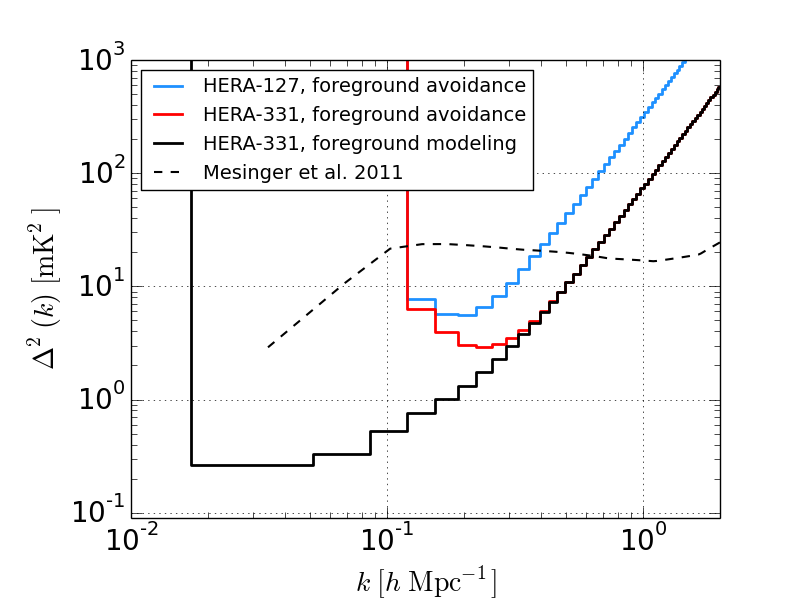
\includegraphics[width=3in]{plots/Pspec/eor_pspec_2014.png}
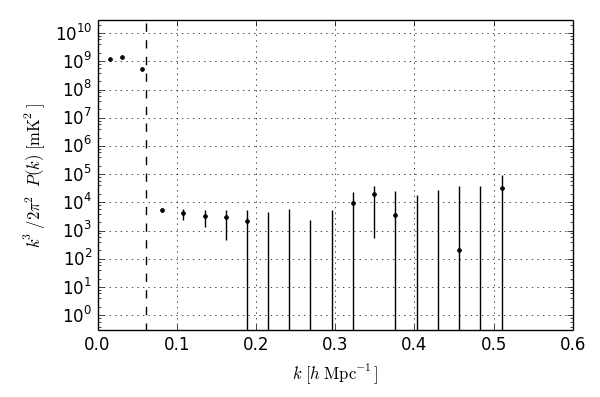
\includegraphics[width=3in]{plots/Pspec/pk_k3pk.png} % XXX trim out left subpanel
\caption{Left: Power-spectrum sensitivities for three stages of
HERA (solid) relative to a fiducial ionization model (dotted line; $\xHI=0.37$, $z=9.0$).  
Sensitivity curves reflect a staged array size and
a staged improvement in analysis software that expands the range
of modes falling into the EoR Window. % XXX haven't described EoR window yet
Right: The current best upper limit on the 21~cm reionization power spectrum,
obtained with a 32-element PAPER deployment \citep{parsons_et_al2013}.  These upper limits
were used to constrain the brightness temperature of the IGM at $z\sim8$, showing
a departure from adiabatic cooling that is presumed to be indicative of X-ray heating.
}\label{fig:eor_pspec}
\end{figure}

A season of observing with HERA-127 will yield high-significance constraints on the 21 cm power 
spectrum across a wide range of k modes and redshifts \citep{pober_et_al2014}.  In Figure \ref{fig:eor_pspec} we show 
the $z=9$ power spectrum predicted by the publicly available 21cmFAST software \citep{mesinger_et_al2011}, 
along with $2\sigma$ HERA sensitivities.  Using the conservative delay-spectrum (``foreground avoidance") 
approach pioneered by PAPER (Parsons et al. 2014), we find that HERA-127 can achieve a $> 10\sigma$ detection 
of fiducial power spectra over a broad range of redshifts.  The subsequent observing season with HERA-331 can 
increase this detection significance to over $25\sigma$ using the same methods.  With detailed foreground 
modeling, the more sophisticated power spectrum estimator developed for the MWA could increase the size of the 
``EoR window", the region of Fourier space with minimal foreground contamination. This would allow for an overall 
detection significance of up to $90\sigma$, along with access to lower $k$ modes and therefore qualitatively 
different physics.  Such a high sensitivity measurement would also allow one to go beyond constraining parameters, 
testing rather than assuming  the underlying theoretical framework and starting to image the large neutral bubbles during reionization.

\subsubsection{Astrophysical parameters from the power spectrum}
%\emph{iii. Various covariance analyses: constraints on different physical processes (Liu/Pober analysis). but
%please -- keep this down to a couple of incisive figures and fiducial models. wall paper doesn't sell very well. }
% Liu, Pober, Dillon

The power spectrum measurements with HERA-331 are sensitive enough to place constraints on theoretical models that 
describe the reionization process.  To first order, the major features of the power spectrum (as simulated by 
21cmFAST) can be parameterized by three terms: $\zeta$, the efficiency at which galaxies release ionizing photons 
into the IGM; $T_{\rm vir}$, the minimum virial temperature of halos that produce ionizing photons (a proxy for 
the minimum mass of the galaxies that drive reionization); and $R_{\rm mfp}$, the mean free path for ionizing 
photons traveling through the IGM, which is determined the prevalence of dense Lyman limit systems.  Current 
observations limit the value of these parameters to within an order-of-magnitude (or worse, in the case of 
$T_{\rm vir}$).  Figure \ref{fig:ErrorEllipses} shows the constraints on each of these parameters achievable 
with multi-redshift HERA-331 power spectrum observations.  We expect to constrain these parameters to better 
than 5\% with a conservative approach to foregrounds, and even better with explicit foreground modeling \citep{pober_et_al2014}.

\begin{figure*}[t]\centering
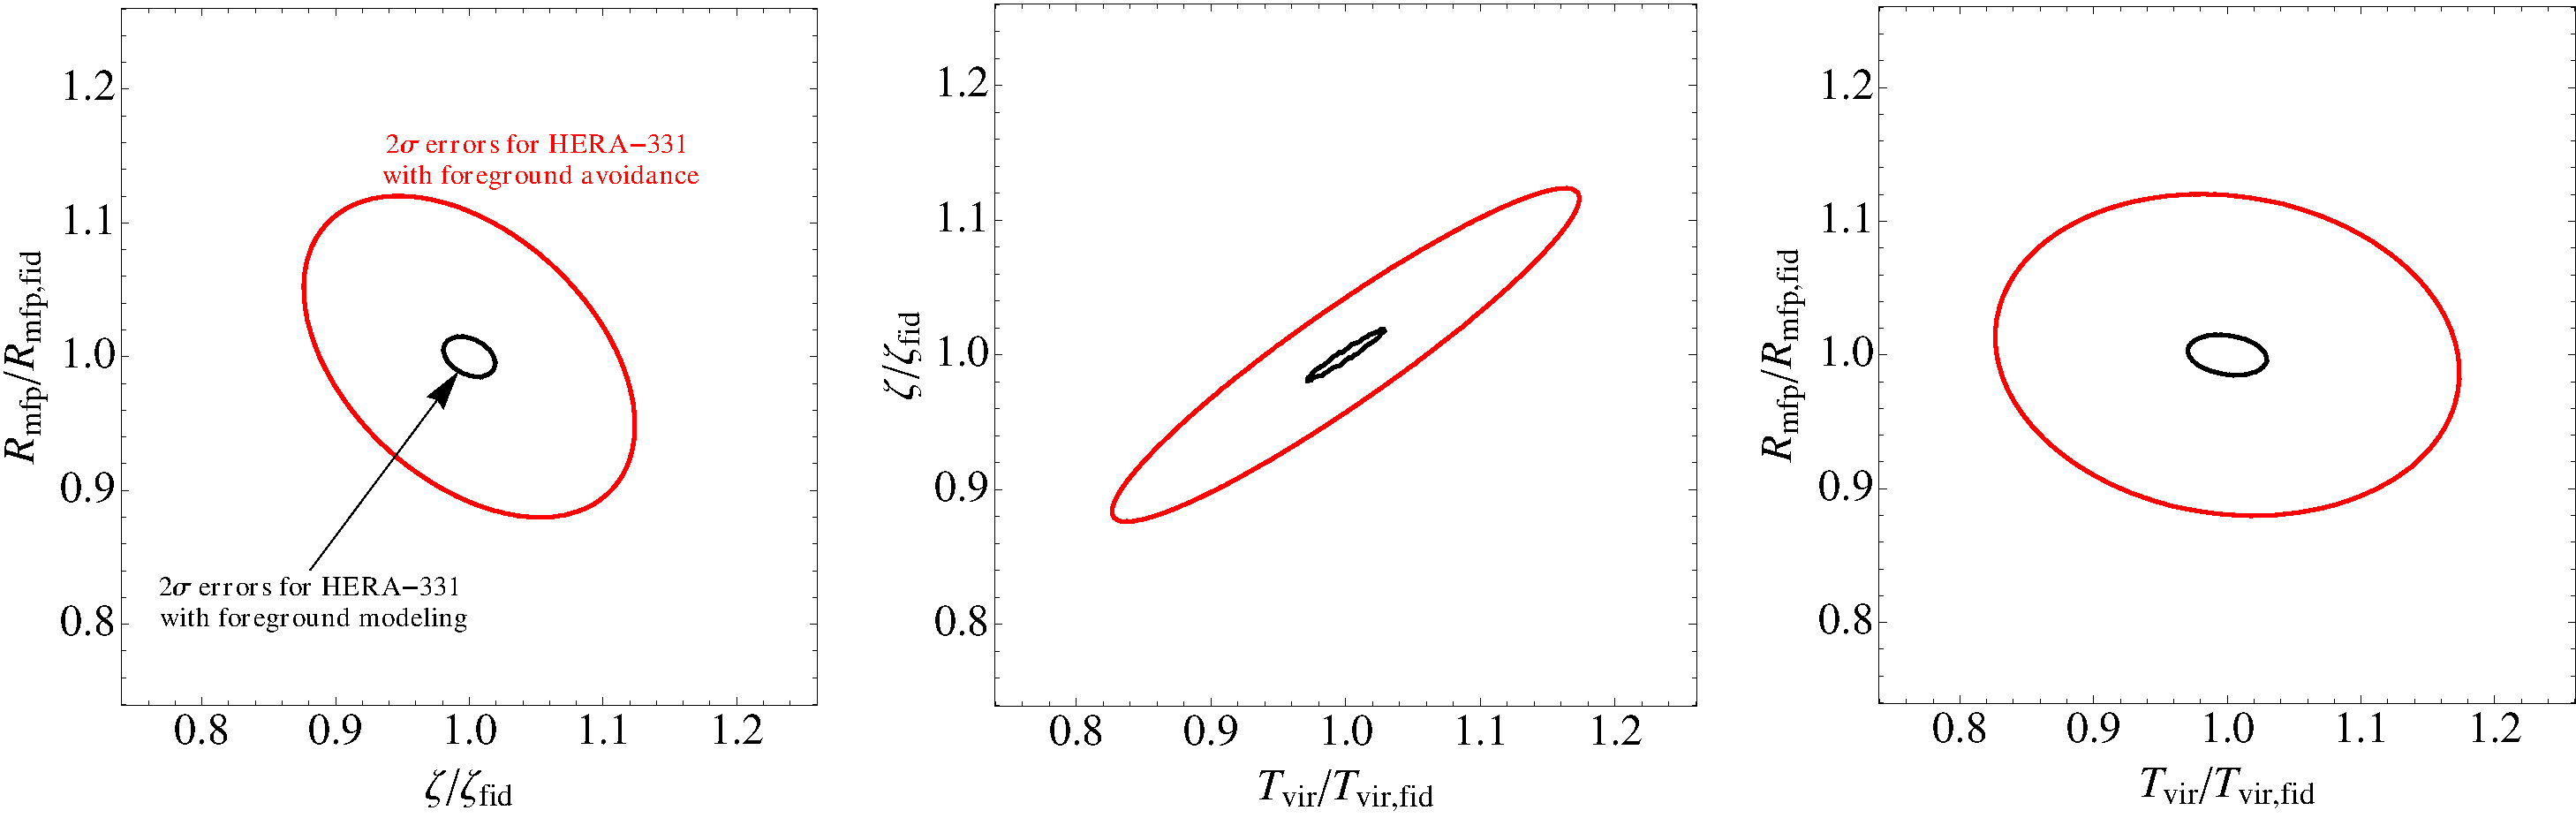
\includegraphics[width=\textwidth]{plots/Pspec/OPTMIDellipses.pdf}
\caption{Pairwise $2\sigma$ error ellipses for $T_{\rm vir}$, $\zeta$, and $R_\textrm{mfp}$, in each case divided by their fiducial values.  HERA-331 projections using existing foreground avoidance techniques are shown in red, while projections using more advanced foreground modeling techniques are shown in black.  The former represent $\sim 5\%$ constraints, while the latter represent $\sim 1\%$ constraints.\label{fig:ErrorEllipses}}
\end{figure*}


% Jacobs
\subsubsection{Imaging HI}
\label{sec:imaging_HI}
%iv. Imaging large scale structure: simulation (Fig) 
With a nearly completely sampled aperture over 300~m across, HERA will have the collecting area of Arecibo but 
with 500x the survey speed it presents the opportunity for directly imaging reionization.  After 100 hours on a 
single field (achievable in 200 nights, or just over one season) HERA will reach a surface brightness sensitivity 
of 50~$\mu$Jy/beam (synthesized beam FWHM $\sim 24'$) compared with typical brightness temperatures of EoR models 
which predicts peaks up to 400~$\mu$Jy/beam.

In imaging, as in the measurement of the power spectrum, noise and foreground residual are comparable limiting 
factors. Using the foreground filtration methods developed for power spectrum estimation, we can remove 
foregrounds exactly as done for the power spectrum estimation --essentially avoiding them in Fourier space-- before imaging.  This ``foreground avoidance'' scheme effectively limits the bandwidth (line of sight 
modes) over which the residuals can be imaged without signal loss.  In Figure \ref{fig:imaging} we demonstrate the 
sensitivity of imaging in this mode assuming a conservative 1MHz of effective bandwidth, 12 Mpc along the line of 
sight.  The brightest structures in the redshift 8 input simulation are detectable at the SNR$>10$ level.

% \begin{figure}[t]\centering
% 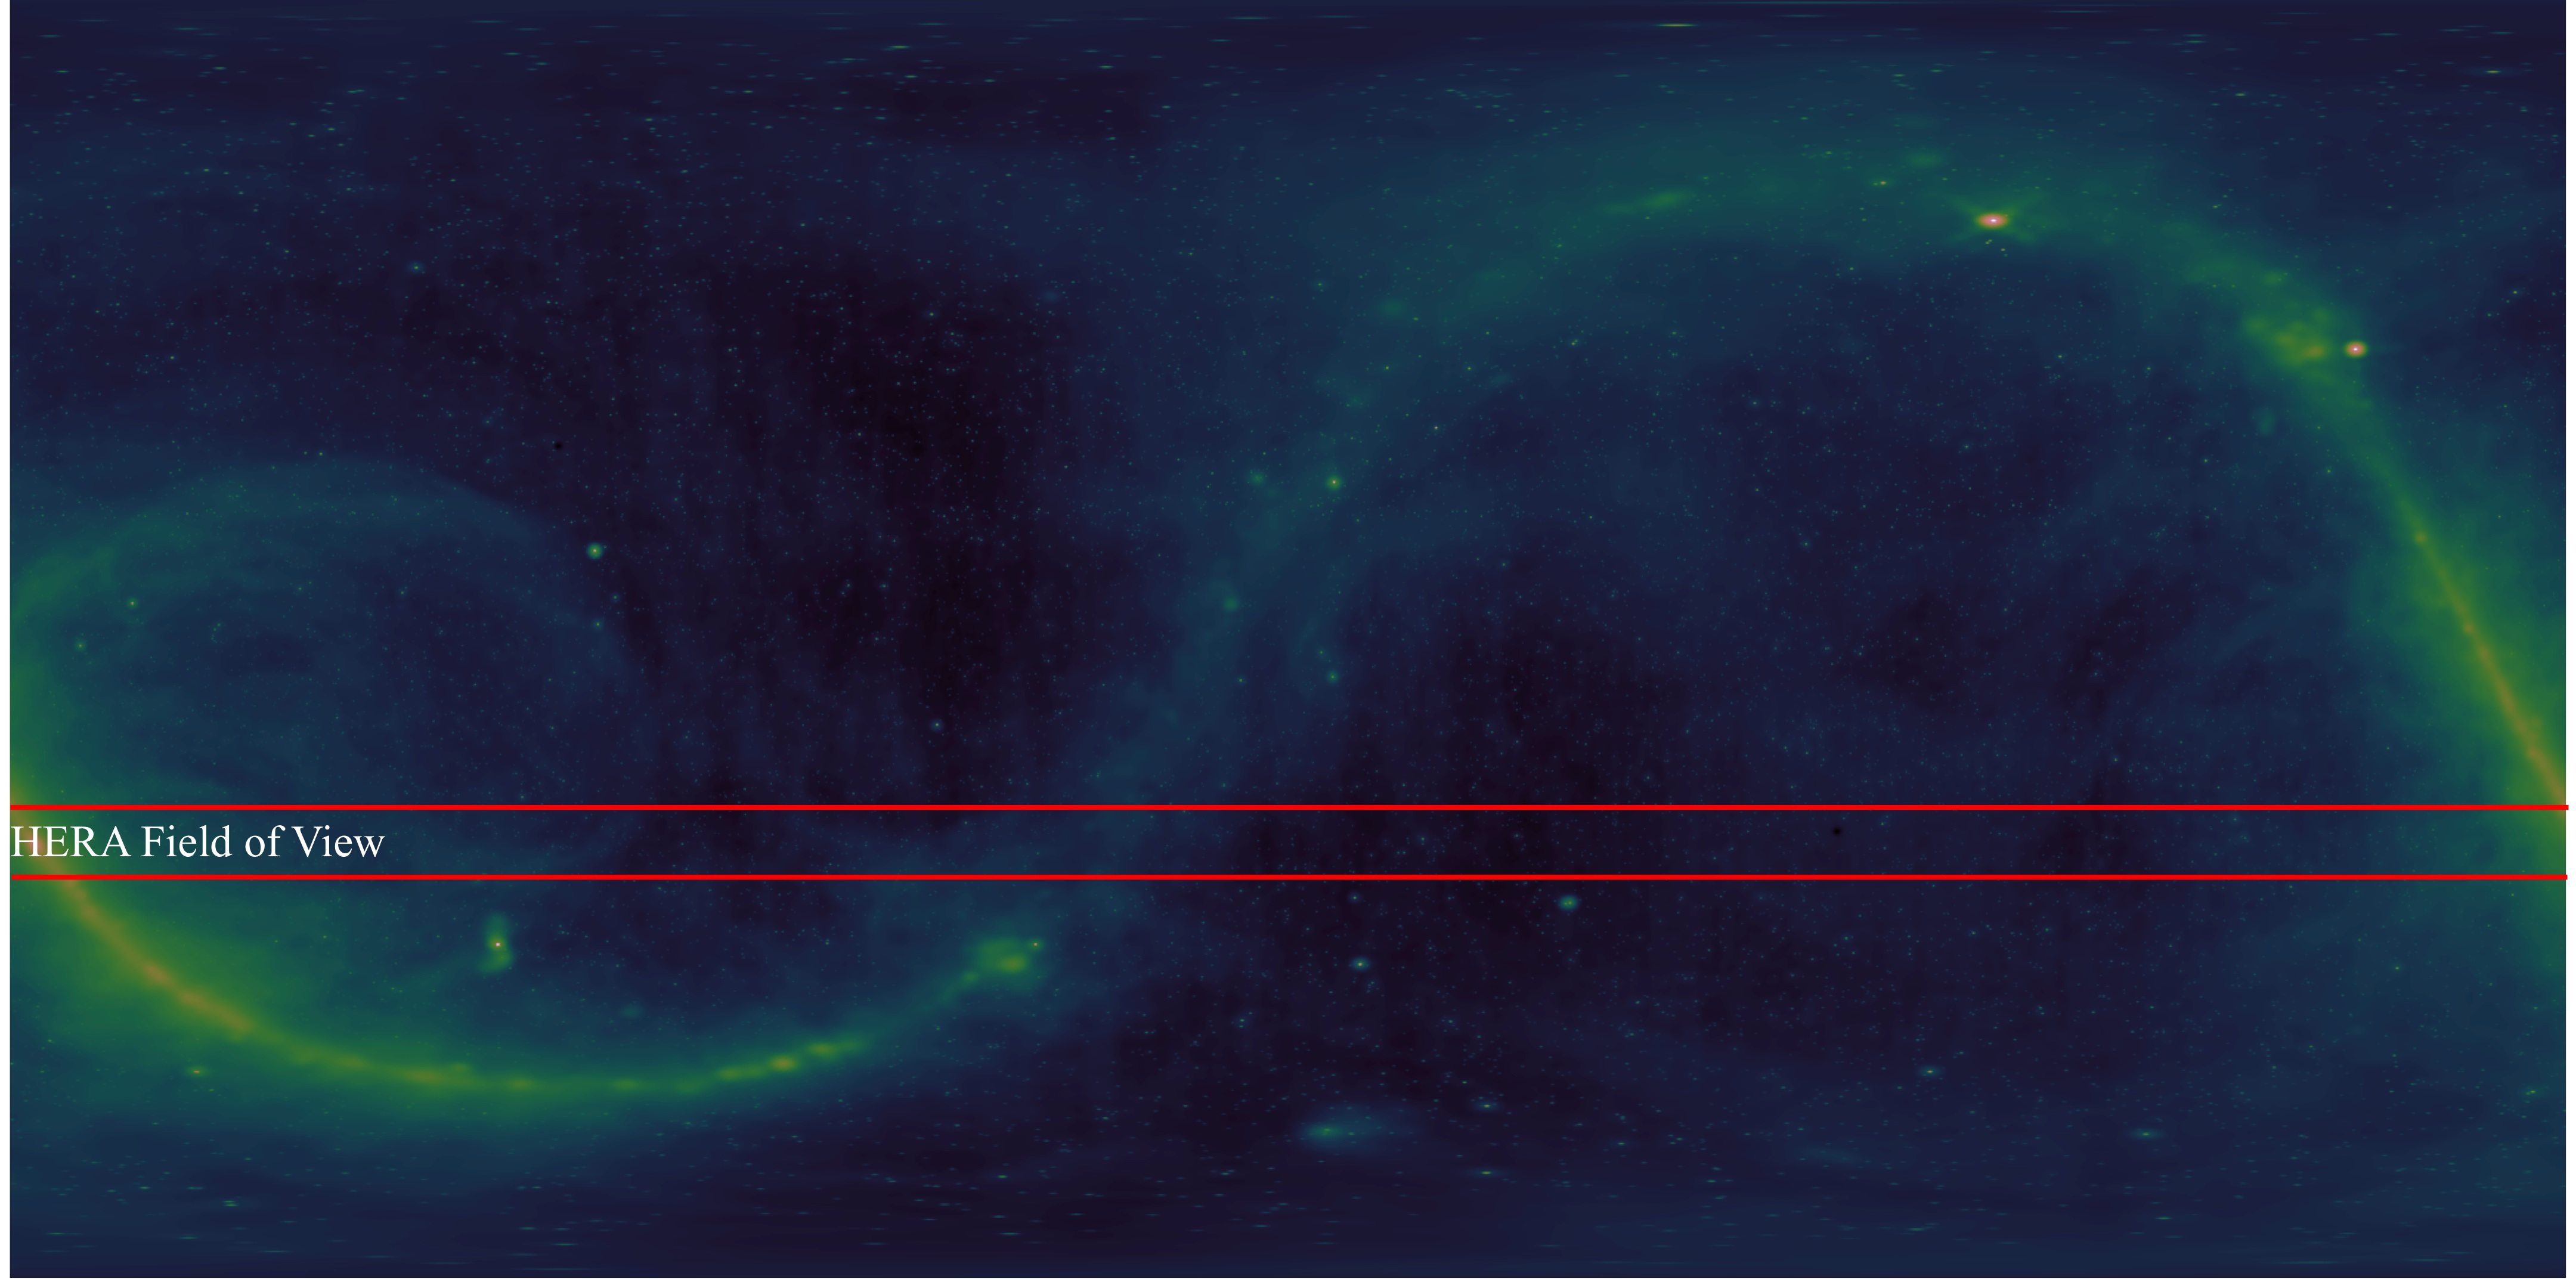
\includegraphics[width=\textwidth]{plots/Imaging/HERA_FoV.jpg}
% % XXX ARP: this figure is way to big.  not sure if it should be in (not enough added information)
% \caption{The HERA stripe.  At 150MHz ($z=8.5$) the HERA field of view is 8\arcdeg.  With a nearly completely sampled aperture over 300m across, HERA will have the collecting area of Arecibo but with 500x the survey speed. Each night it will drift scan 2600 square degrees for a survey volume of 50 $Gpc^3$.  The stripe includes the GOODs south field, one of the best studied regions of sky. \label{fig:HERA_FoV}}
% \end{figure}

\begin{figure}[!ht]\centering
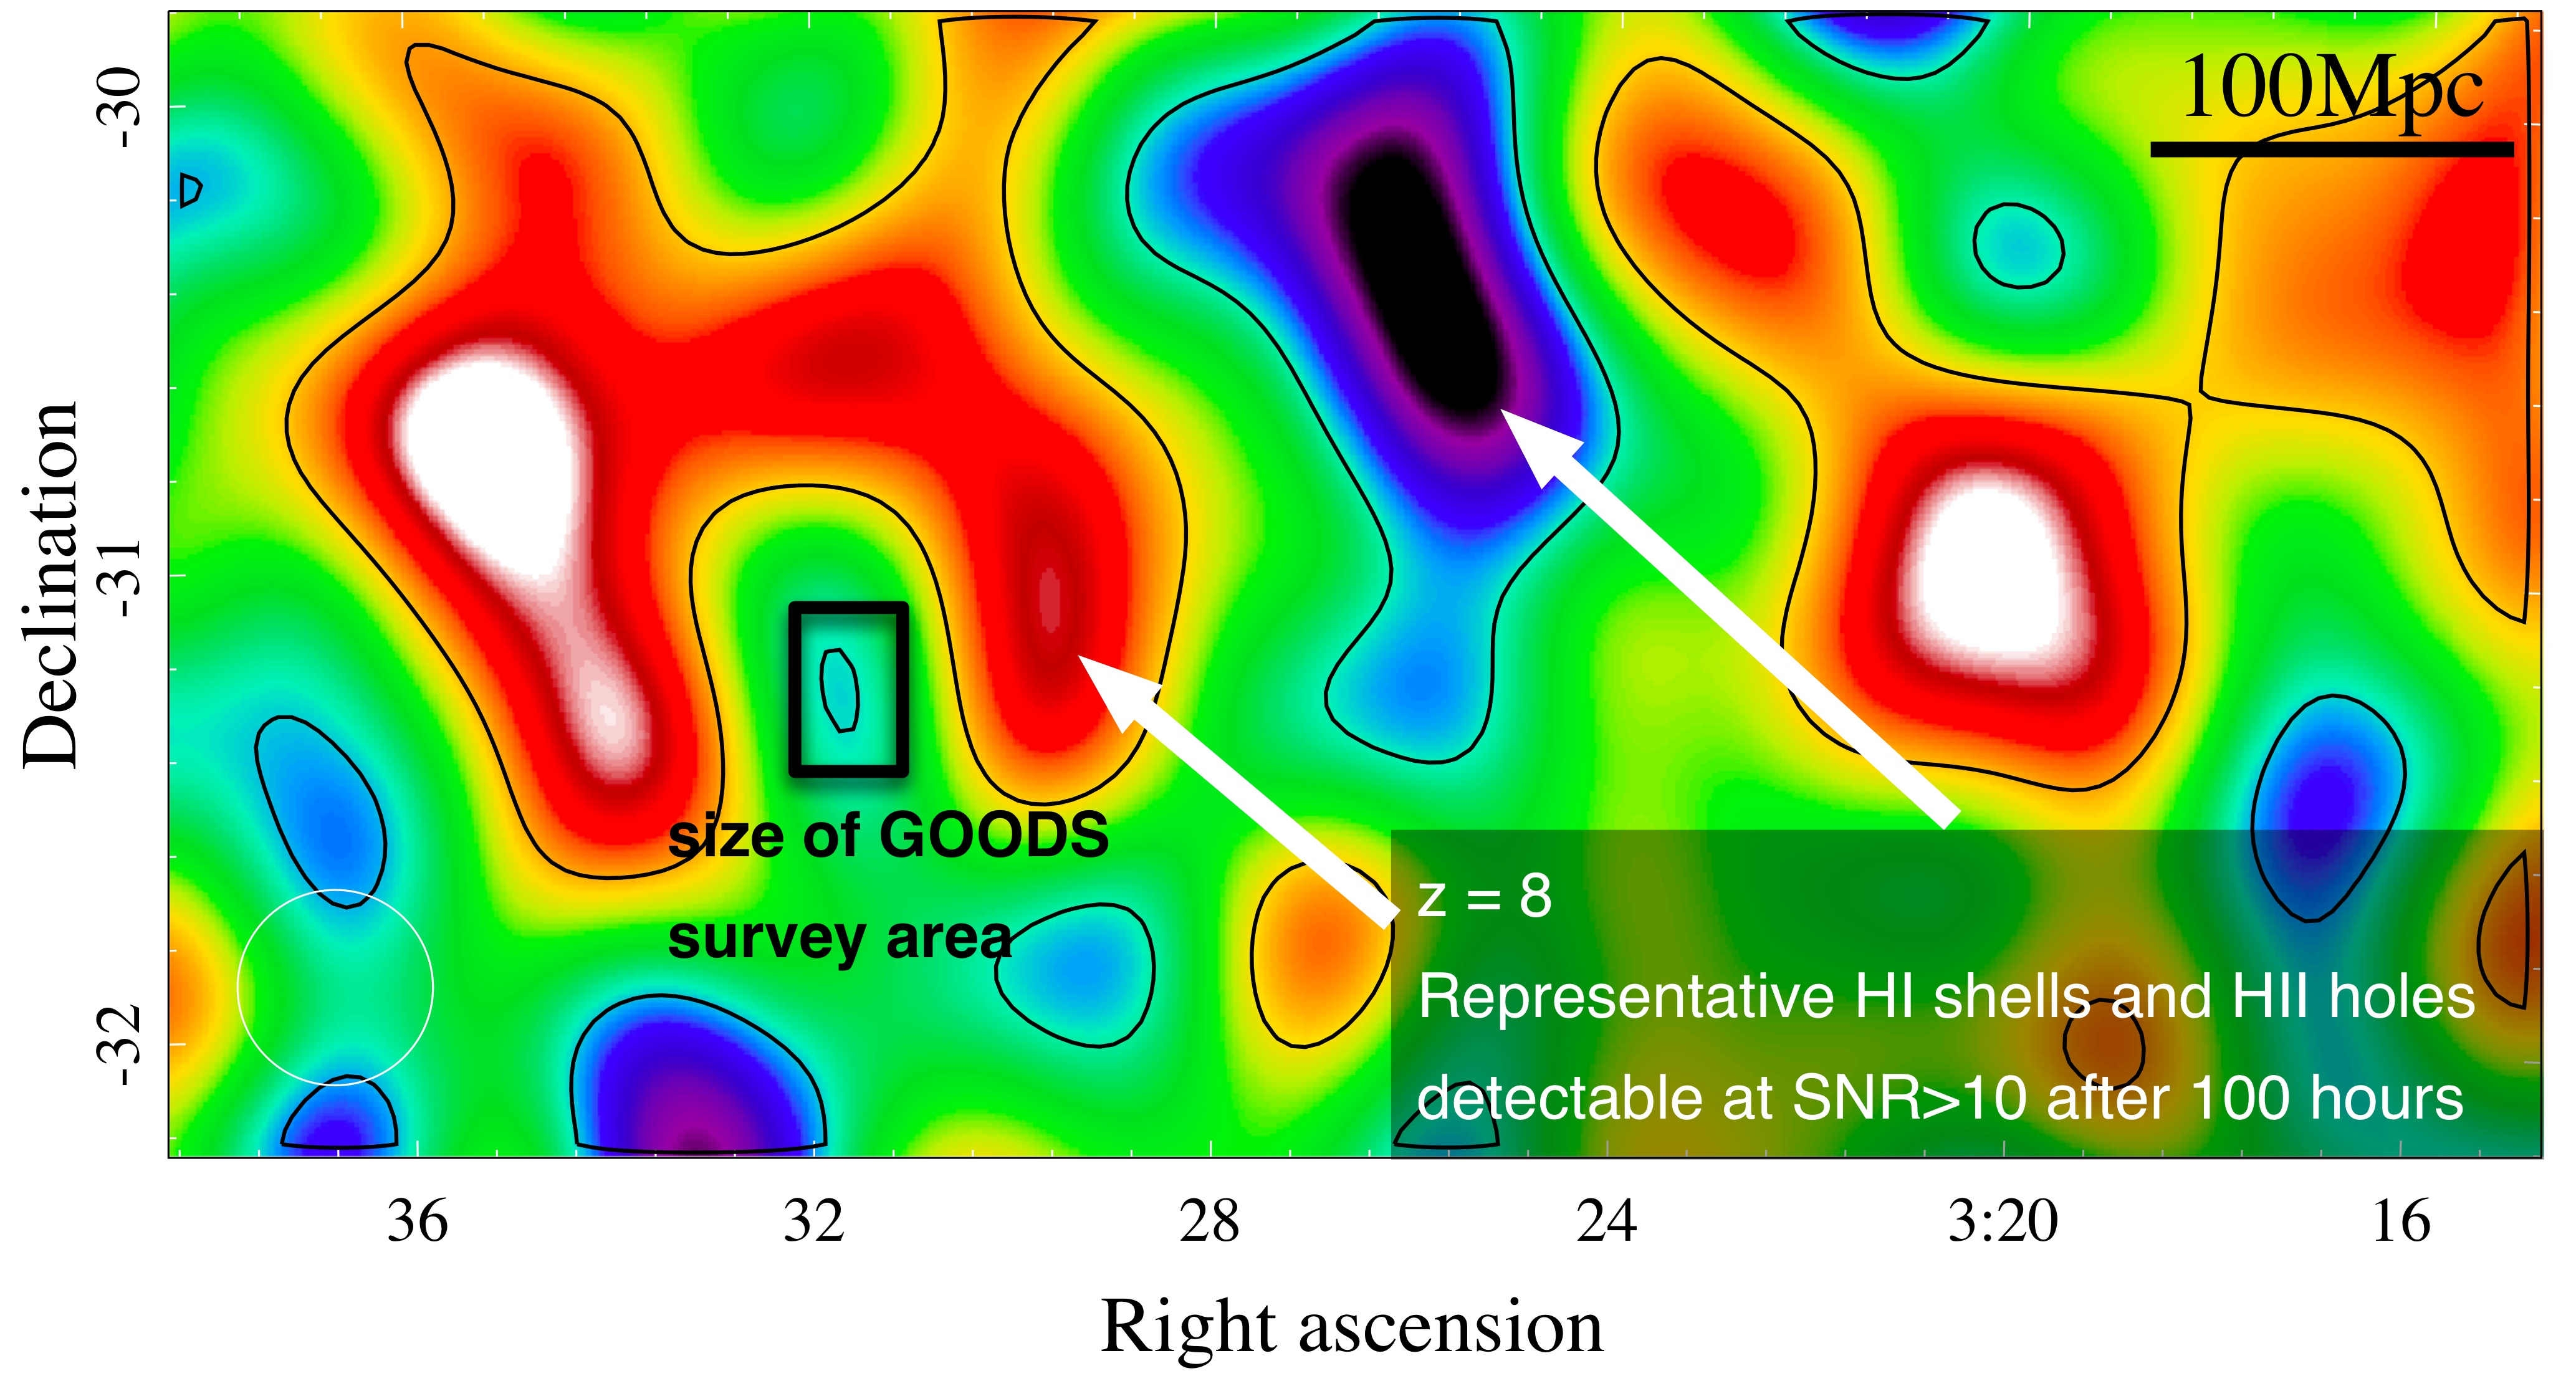
\includegraphics[width=\textwidth]{plots/Imaging/HERA_331_z8_SNR_annotated.jpg}%HERA_331_z8_SNR_annotated.jpg}
% XXX need to cut this down to just the imaging sim, I think
\caption{\small
With sensitivity highly concentrated at the largest scales, HERA is capable of directly imaging HI during reionization.  Shown here is a simulation of EoR emission \citep{mcquinn_et_al2007} as imaged by HERA with noise equivalent to 100 hours of observation.  
Contours enclose regions with signal to noise above 10.  The regions detected on scales of $\sim$100~Mpc bracket the size scales probed by deep galaxy surveys.  At 150~MHz ($z=8.5$) the HERA field of view is 8\arcdeg.  With a nearly completely sampled aperture over 300~m across, HERA will have the collecting area of Arecibo but with $500\times$ the survey speed. Each night it will drift scan 2600 square degrees for a survey volume of 50`$Gpc^3$.  The survey area includes the GOODS-South field \citep{dickinson_et_al2003} (denoted by the black rectangle).  As one of the best studied regions of sky, the GOODs-South survey volume includes 179 known objects above $z=7$, which represents $\sim45\%$ of all such objects over the entire sky.}  \label{fig:imaging}
\end{figure}    

%
%\begin{figure}[!ht]\centering
%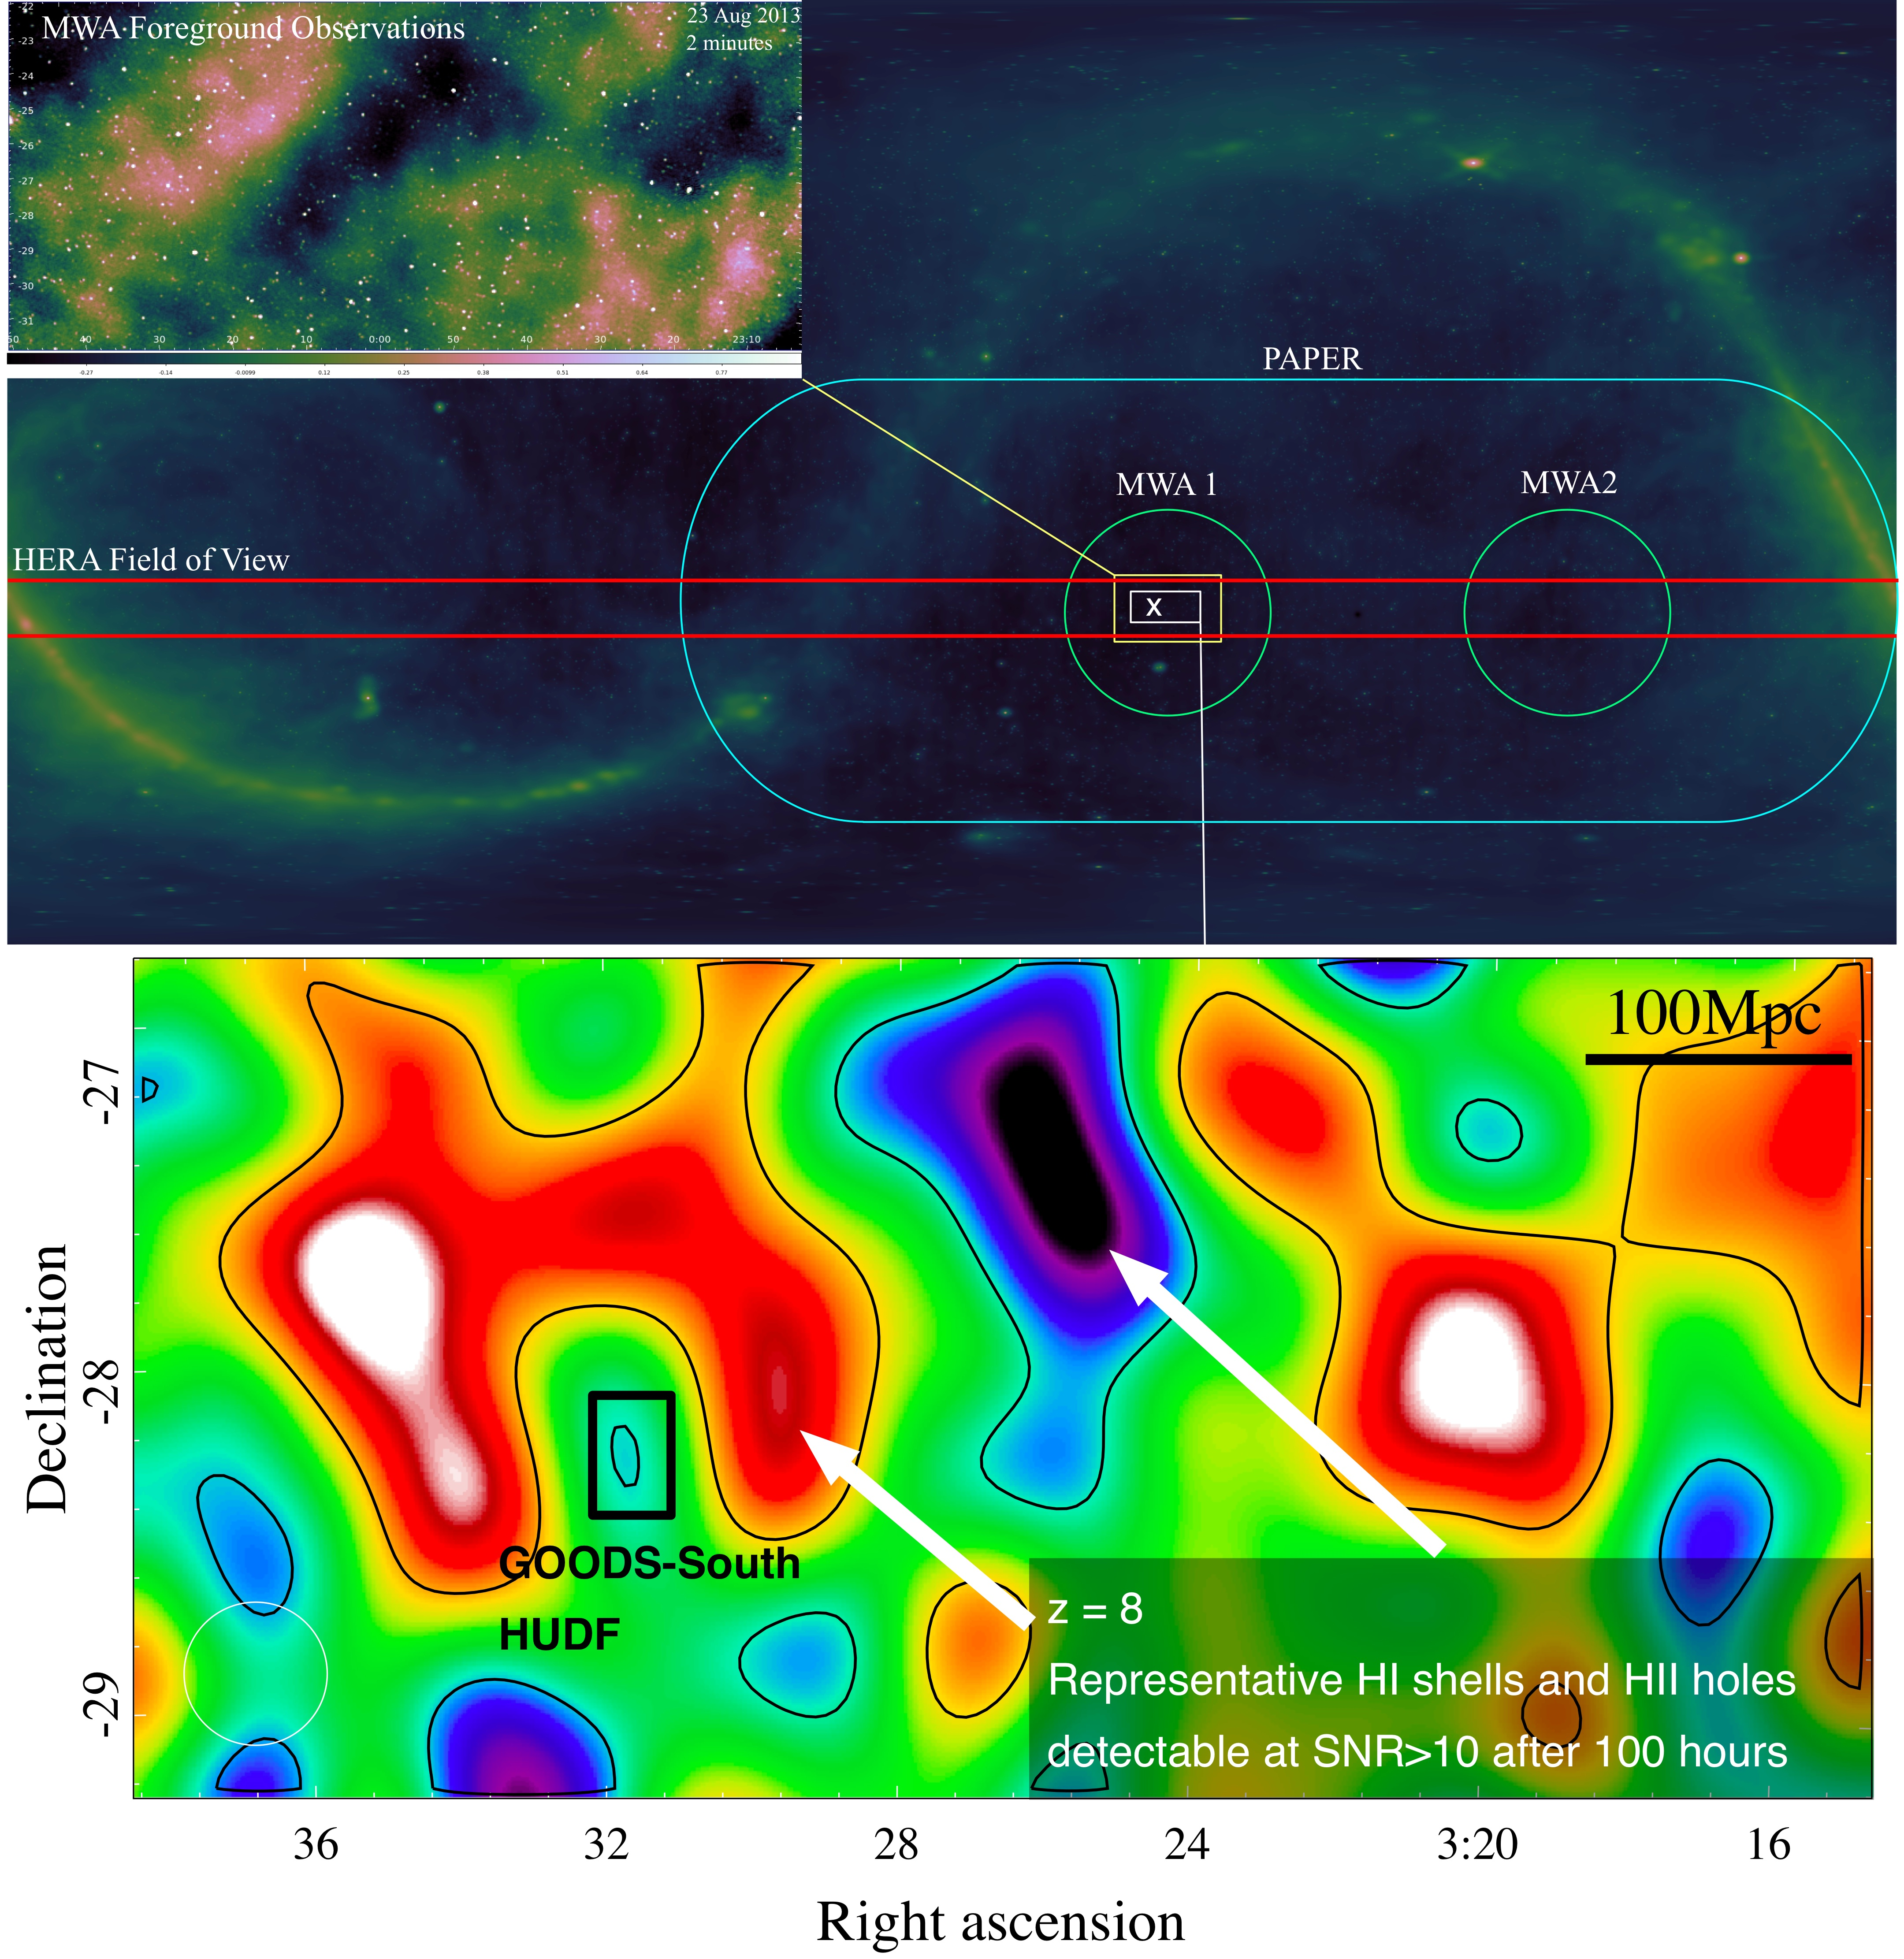
\includegraphics[width=\textwidth]{plots/Imaging/HERA_FoV_and_sim.jpg}%HERA_331_z8_SNR_annotated.jpg}
%% XXX need to cut this down to just the imaging sim, I think
%\caption{\small
%With sensitivity highly concentrated at the largest scales, HERA is capable of directly imaging HI during reionization.  Shown here is the HERA ``stripe''.  At 150~MHz ($z=8.5$) the HERA field of view is 8\arcdeg.  With a nearly completely sampled aperture over 300~m across, HERA will have the collecting area of Arecibo but with 500x the survey speed. Each night it will drift scan 2600 square degrees for a survey volume of 50`$Gpc^3$.  The stripe includes the GOODS-South field \citep{dickinson_et_al2003}, one of the best studied regions of sky.  Shown here is a simulation of EoR emission \citep{mcquinn_et_al2007} as imaged by HERA with noise equivalent to 100 hours of observation.  
%Contours enclose regions with signal to noise above 10.  The regions detected on scales of $\sim$100~Mpc are bracket the size scales probed by deep galaxy surveys (cf. the GOODs-South survey volume where 179 objects about $z=7$ have been detected, representing $\sim45\%$ of all such objects over the entire sky.)}  \label{fig:imaging}
%\end{figure}    

%\subsubsection{Imaging as a probe of non-gaussianity}
%\emph{a) Imaging as a probe of non-Gaussianity and topology of reionization (Fig from Watkinson \& Pritchard)
%[Not sure if this belongs here, should discuss: b) Bayesian imaging (Figs from Paul Sutter).  
%Perhaps a broader impact on the radio community too?]}
%% Morales, Tegmark

\subsubsection{Early IGM heating: back to the Dark Ages}
%\emph{v. Approaching Dark ages (z=20 to 30): early Xray heating? other (Fig - Liu models)}
% Liu, Dillon, Hewitt
%\begin{figure}[t]\centering
%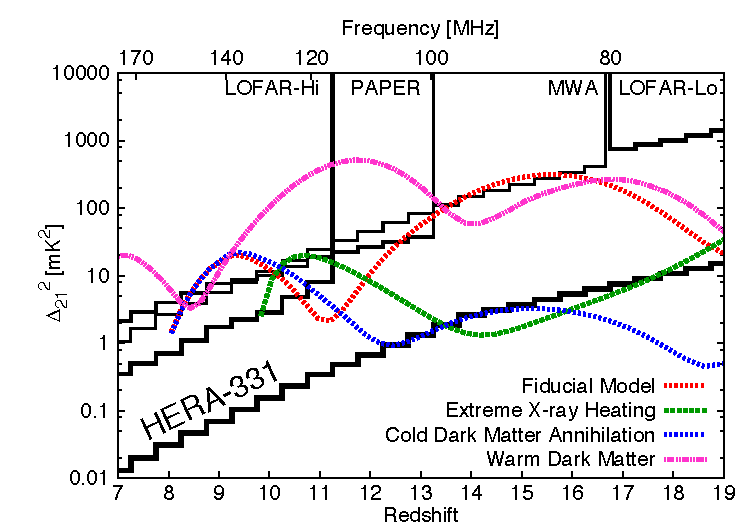
\includegraphics{plots/Xray/HERA_II_compare_kp1_whoriz_20pt.pdf} 
%\caption{\small 
%At low frequencies, HERA opens a window to
%pre-reionization physics at the end of the Dark Ages. Plotted are power spectrum amplitudes (at $k =
%0.15h$~Mpc$^{-1}$) for various IGM heating models \citep{mesinger_et_al2013},
%with predicted HERA sensitivities.
%% XXX maybe merge this back in with x_i vs z figure in dark ages subsection
%}\label{fig:Xray} \end{figure}

With high sensitivity throughout the observing band, HERA represents an opportunity to push the redshift 
frontier of current-generation instruments, extending observations to the pre-reionization era ($z \sim 20$)
in an  uninterrupted way.  Doing so will allow a measurement of an earlier peak in the $21\,\textrm{cm}$ power 
spectrum, corresponding to an era of IGM heating from various X-ray sources.  Theoretical expectations 
span a wide range of possible scenarios for IGM heating. Figure \ref{fig:x_i_vs_z} shows several possibilities that 
were examined in \cite{mesinger_et_al2013}, with HERA's sensitivity overlaid.  
Heating is likely dominated by X-rays from black
hole binaries, but could have a strong, easily-identified contribution from
Dark Matter annihilation in some models \citep{mesinger_et_al2013}.  Additionally, the early redshifts
corresponding to the Cosmic Dawn are great testbeds for popular LCDM
alternatives, such as Warm Dark Matter, as the Universe is expected to be empty
in these models.  This makes the 21~cm signal during the pre-reionization Cosmic
Dawn epoch a powerful probe of both astrophysics and cosmology. 

As seen in  Figure \ref{fig:x_i_vs_z}, the HERA 21~cm observations are sensitive to 
the rate and density of massive black holes formed in the
early universe \citep{pritchard_loeb2010} via their X-ray emission (see Figure \ref{fig:x_i_vs_z}, right panel), 
how velocity streaming between baryonic 
matter and the dark matter halos affected early structure formation and the onset
of Ly$\alpha$ emission \citep{visbal_et_al2012}, and will lay the groundwork for future
efforts to explore how 
cosmological models can be improved via measurements of redshift-space distortions,
artificial anisotropies introduced via the Alcock-Paczy\'inski effect, and
gravitational lensing signals\citep{furlanetto_et_al2006}.

%vi. 21~cm forest: perhaps a paragraph on possibilities of small scale structure, if we can find radio galaxy? (Fig) 
% Carilli, Furlanetto -- Forget it.  Too much explanation needed. 

\subsubsection{Cross-correlation Science}
\label{sec:CrossCorrelation}
%vii. Cross-correlation science: 

The ability of HERA to image enables an exciting range of cross-correlation science. 
HERA HI images reveal the large-scale reionization environment for pointed ALMA and JWST 
observations, and other deep near-IR surveys \citep{lidz_et_al2009}.  
Knowing whether an observed galaxy is in a region that  was
previously reionized (center of large HII bubble), recently reionized (edge of HII bubble), or is forming from 
pristine neutral gas provides important contextual information on early galaxy formation.

The HI images can be ross-correlate with other diffuse 
tracers of large scale structure.  A number of studies have proposed cross-correlation with large scale intensity
mapping of molecular  CO \cite{lidz_et_al2011} and atomic CII \citep{gong_et_al2011} lines. 
Prototypes of these experiments 
may be operating on the HERA timescale.  Such probes have the advantage of having different systematics 
compared to HERA, potentially allowing clean measurements of the underlying signal.

%b. CMB pol 
%Cross-correlations with the optical depth measurements \citep{sarkar_et_al2009,meerburg_et_al2013}
% CMB omitted because most studies look way too optimistic.  Probably not going to happen.  ACL
% c. CO/CII IM: optimistic or wrong timescale? 
%e. Anscillary science with PAPER 128: transients, solar 
% de Boer
%\clearpage

%  _                           
% | |   ___ ______ ___ _ _  ___
% | |__/ -_|_-<_-</ _ \ ' \(_-<
% |____\___/__/__/\___/_||_/__/

\section{Achievements Under Prior NSF Support} % this is a required section of the proposal
%\section{Why build HERA now, and the lessons from MWA \& PAPER}
%\subsection{Where we are right now: PAPER, MWA}  % 2 pages
%\section{Foregrounds \& Lessons Learned from PAPER and MWA} 
\label{sec:Lessons}

\begin{figure}[t]\centering
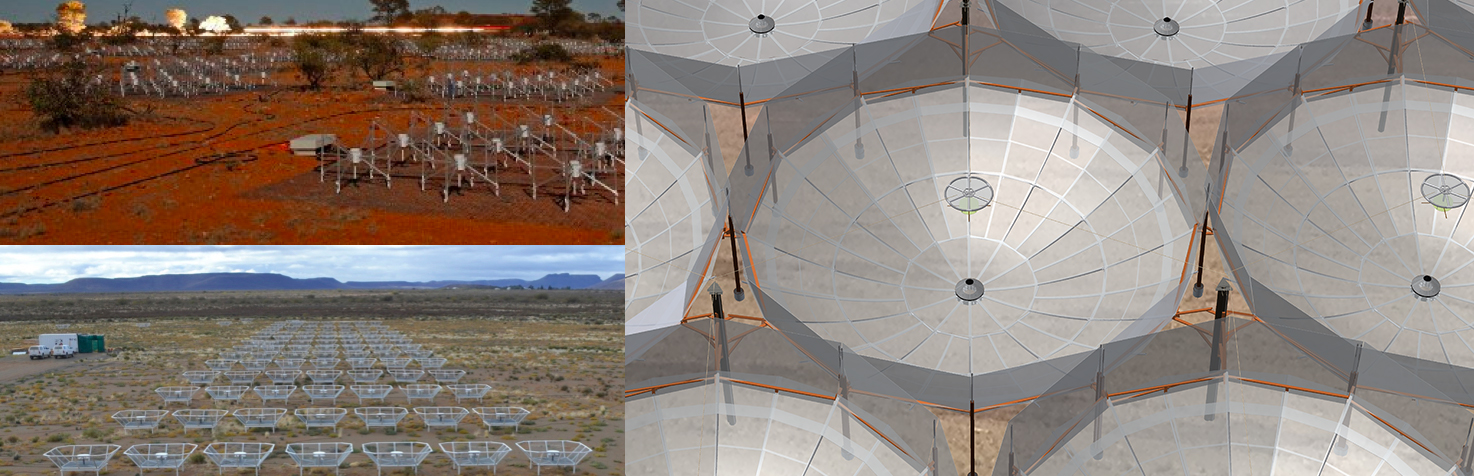
\includegraphics[width=6.5in]{plots/PAPER_and_MWA_and_HERA.jpg}
\caption{\small
The MWA (top left) and PAPER (bottom left) arrays, each currently deployed with 128 elements.
The 14-m HERA element (right) dramatically improves sensitivity while 
constraining the path length and amplitude of reflections to ensure that foreground
isolation is not substantially degraded.
%The core of HERA~331 consists of a redundant hexagonal array with
%outrigger antennas (not shown) for imaging and foreground mitigation.
}
\label{fig:hera_dish}
\end{figure}


The HERA project team consists of PIs and technical leaders from four NSF-funded projects targeting the 21cm signal
at high redshifts:
\begin{itemize}[noitemsep,nolistsep]
% XXX list PIs/tech leads as well?
\item{PAPER:} (NSF grants \#1129258, \#0804508, \#0607838, and \#0505354) PAPER efforts began humbly with a 4-element
array deployed in Green Bank, WV.  Following a cycle of incremental
development, testing, and deployment, PAPER has upgraded and optimized nearly every aspect of its system, using the Green Bank site
for technical development and testing.  In 2009, PAPER deployed a 16-element, single-polarization interferometer in South Africa
near the planned site of the Square Kilometre Array (SKA) mid-band telescope.  
Since then, PAPER has doubled its size annually for four years running.  As of Nov. 2013, PAPER's primary science
deployment in South Africa consists of 128 dual-polarization, zenith-pointing dipoles arrayed in a sparse redundant configuration
(Figure \ref{fig:hera_dish}, bottom left; \citealt{parsons_et_al2012a}).  PAPER pioneered the use of redundant configurations
to maximize array sensitivity for power-spectrum measurements, the use of drift-scanning elements with associated powerful
analysis techniques, a scalable correlator architecture that has enabled arrays to inexpensively grow exponentially
with Moore's Law, and a data compression scheme that reduces data volume by a factor of $\sim$40 without impacting
reionization science.  Perhaps most importantly, PAPER pioneered the delay-spectrum foreground avoidance technique \cite{parsons_et_al2012b}
% XXX maybe defer the 4-orders-of-mag for later
that in recent PAPER observations has been demonstrated to suppress foregrounds by at least 4 orders of magnitude 
(Figure \ref{fig:eor_pspec}; \citealt{parsons_et_al2013}).  The resulting power spectrum is the most stringent upper
limit on reionization by almost two orders of magnitude in mK$^2$, and was used to show that the early IGM must have
been heated prior to reionization --- presumably by emission from high-mass X-ray binaries.

\item{MWA:} (NSF grants \#0457585, \#082132, \#1109257) 
The MWA is a dipole-based aperture array synthesis telescope designed
to operate in the 80--300~MHz frequency range.
It is located at the
Murchison Radio-astronomy Observatory (MRO) in Western Australia, the
planned site of the future SKA low-band
telescope, and is one of three telescopes designated as a pathfinder
for the SKA. 
The MWA has been developed by an international collaboration,
including partners from the United States, India, Australia, and New
Zealand, and consists of
128 digitally steerable antenna tiles arranged in a centrally
condensed but highly randomized layout (Figure \ref{fig:hera_dish}, upper left;
\citealt{tingay_et_al2013_trunc}). The randomized layout and synthesis rotation
from tracked observations provide a filled $uv$-plane and excellent
full-polarization imaging of the foregrounds.
The MWA's hardware performance \citep{bowman_et_al2007a}, calibration pipeline
\citep{mitchell_et_al2008}, and foreground subtraction strategy \citep{morales_et_al2006a}
have been extensively documented and investigated
in existing literature.
The US MWA team has been a world leader in the application of 
foreground subtraction for
enlarging the EoR window---qualitatively increasing the science % XXX EoR window used before defined
reach of the power spectrum and enabling imaging of reionization (Figure
\ref{fig:eor_pspec}). The resulting analysis is more complex than the
delay-spectrum approach (e.g.\ \citealt{hazelton_et_al2013}) but naturally
removes polarized foregrounds \citep{moore_et_al2013} and enables the
comparison with observations at other bands. Recent MWA observations have
demonstrated the use of image-based modeling (Figure \ref{fig:twoFGViews}, left) to
subtract foregrounds to the thermal noise limit 
within certain regions of the foreground wedge (Figure \ref{fig:twoFGViews}, right). % XXX this mention of wedge comes before description

\item{MITEoR:} (NSF grants \#0908848, \#1105835) MITEoR is a novel effort aimed at
examining new cross-correlation and calibration techniques for low-frequency radio telescope
arrays such as those targeting 21cm reionization.  These techniques are being applied
to a deployed 64-element array based on MWA dipole elements.  While spatial-FFT-based cross-correlation
techniques remain under development, MITEoR brings to HERA critical expertise in the area
of calibration on the basis of redundancy, as well as optimal quadratic power spectrum estimation techniques.

\item{LEDA:} (NSF grant \#1106045). LEDA is a technology-driven effort to solve aspects of calibration relating
to an experiment targeting the global 21cm reionization signature.  With Werthimer leading the digital effort,
LEDA has pioneered the application of graphics processing units (GPUs) in correlator architectures, developing
and deploying a heterogeneous computing system that fully correlates 256 dual-polarization elements.  This
technology has been adopted into recent PAPER correlator deployments, and will be applied to HERAs correlator
and data compression system.
\end{itemize}
Other successful efforts by members of the HERA project team include the EDGES experiment (NSF grants \#0905990, \#1207761),
the Center for Astronomy Signal Processing and Electronics Research (NSF grant \#0906040), the Advanced Multibeam
Spectrometer for the GBT (NSF grant \#1006509), and numerous other efforts.
All of these efforts have undertaken significant development of hardware systems and have 
successfully completed major deployments.  Members of the project teams of each of these projects
bring to HERA mature hardware designs, software pipelines, and powerful analysis frameworks that
have come from the successful execution of these funded projects.  
In accordance with their scope,
these projects also have a strong record of ground-breaking research, with a sizeable record in the published literature.
Finally, HERA's leadership brings substantial experience
collaborating internationally, managing the design, development, testing, and integration of complex systems,
adhering to project timelines and budgets, and setting incremental development and deployment plans that
ensure that progress is made on a predictable schedule, with time to adapt to contingencies.

% XXX Broader impacts of prior support


\subsection{Lessons for HERA}

% XXX goal: trim out mention of wedge before here, except for a very brief mention in overview

\begin{figure}[t]\centering
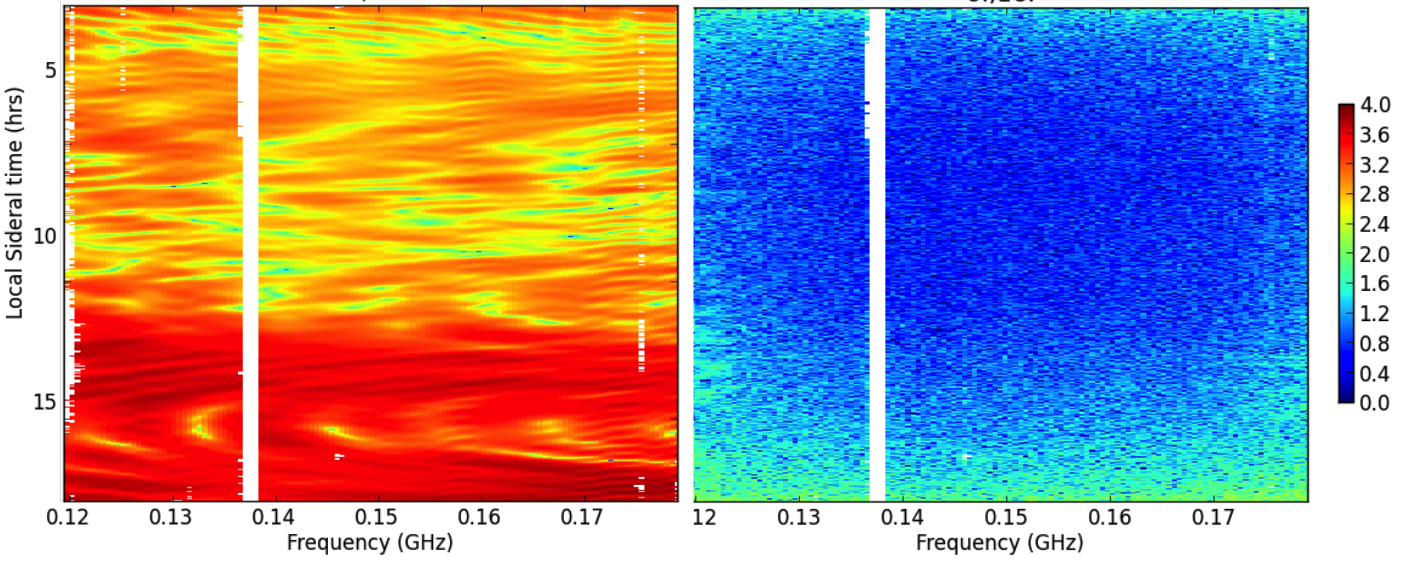
\includegraphics[width=6in]{plots/waterfall_filtered.png}
\caption{\small 
Waterfall plots illustrating, as a function of time and frequency, PAPER visibilities
measured on a 30-m baseline before (left) and after (right) the application of a 
filter that removes forground emission within the wedge.  Color scale indicates amplitude in $\log_{10}({\rm Jy})$.
This filter has been shown to suppress
foreground systematics by 4 orders of magnitude, leaving residuals demonstrably noise-dominated.
}\label{fig:waterfall} \end{figure}


The key challenge of 21~cm cosmological reionization experiments is 
balancing the collecting area needed to detect the faint 21~cm reionization signal
with the precision needed to suppress
% XXX this figure doesn't really quantify # of orders of magnitude
foregrounds that are $\sim$5 orders of magnitude brighter \cite{deolivieracosta_et_al2008}.
The major breakthrough in 21~cm cosmology---what enables us to propose HERA now---is 
the discovery of how 
instrumentation and analysis can exploit the 
spectral smoothness of foregrounds
to open up an `EoR Window'.  
%These advances have been pioneered by the MWA and PAPER teams \citep{morales_et_al2012,parsons_et_al2012b,vedantham_2012,Datta_2010,hazelton_et_al2013,pober_et_al2013,parsons_et_al2013,dillon_et_al2013b}, and enable us to design a targeted HERA instrument that can reveal the details of reionization (Figure \ref{fig:x_i_vs_z}) and image the largest structures (Figure \ref{fig:imaging}).
% XXX better phrase for "EoR window"?
As illustrated in Figure \ref{fig:waterfall}, these advances have been used to suppress foreground emission by 4
orders of magnitude in PAPER observations,
with results that begin ruling out certain reionization scenarios
\citep{parsons_et_al2013}.

Observations for 21~cm cosmology experiments are best understood in
Fourier space.  Because the \HI emission is a
narrow spectral line, the observed frequency of the emission can be mapped to
redshift or line-of-sight distance to provide an observed volume $\{x,y,z\}$ in
comoving Mpc. This observed volume is Fourier transformed into a 3D
wavenumber cube $\k\equiv\{k_{x}, k_{y}, k_{z}\}$. For graphical simplicity, the angular
wavenumbers are typically averaged ($\{k_{x},k_{y}\}\rightarrow\kperp$) to
produce line-of-sight wavenumber $\kpar$ vs.\ angular $\kperp$. 
%Interferometric measurements are of the angular Fourier modes in many
%frequency channels (visibilities), so in the absence of widefield effects only
%a Fourier transform in the frequency direction and a coordinate mapping is
%needed to obtain the 3D $\{k_{x}, k_{y}, k_{z}\}$ measurements
%\citep{morales_hewitt2004}.) 
The expected statistical isotropy of the signal allows measurements in $k$-space to be
squared and averaged in shells to produce the spherical power spectrum
shown in Figure \ref{fig:eor_pspec}.

Through a concerted theoretical and observational campaign by the PAPER and MWA teams
\citep{morales_et_al2012,parsons_et_al2012b,vedantham_2012,Datta_2010,hazelton_et_al2013,pober_et_al2013,parsons_et_al2013,dillon_et_al2013b}
we now understand that foreground contamination can be confined to a `wedge' in
$\kpar$ vs.\ $\kperp$, as demonstrated by the PAPER observations in the
righthand panel of of Figure \ref{fig:twoFGViews}. 
%MM: a figure showing results from both arrays would be really powerful here.
This wedge is the result of
the smooth spectrum foregrounds 
%XXX SF: I would make this more obvious.  I recommend replacing this sentence with something like (with my naive understanding): "This sharp division occurs because foregrounds have smooth spectra (which cause the sources to manifest at small $\kpar$), some of which is projected into the transverse direction ($\kperp$) through the instrument's well-understood chromatic properties."
(low $\kpar$) interacting with the inherent
chromaticity of an interferometer. 
This leaves the region above the wedge free from 
foreground emission---a window through which we can observe the EoR. 
As demonstrated in the right-hand panel of Figure \ref{fig:waterfall}, removal of the foreground wedge 
directly suppresses foregrounds by at least 4 orders of magnitude.
We now understand the source of the EoR window, how we can increase the 21~cm signal region, and have seen the window in observations with both PAPER and the MWA \citep{pober_et_al2013,dillon_et_al2013b}.

The time is now ripe for an experiment that builds from the technical heritage
of PAPER, the MWA, MITEoR, and LEDA, and incorporates into the design of the
instrument new insights relating to the interplay of sensitivity and the
foreground wedge.  HERA's new 14-m dish, whose design is motivated by the core
tenets delay-spectrum foreground avoidance, is foundational to this effort.
These elements, arranged redundantly in a compact hexagonal grid, enable both the
delay-spectrum foreground avoidance and calibration from PAPER (redundant
baselines, proven performance, low risk) and the foreground subtraction and
imaging from the MWA (filled $uv$~coverage, higher sensitivity and immunity to
polarized foregrounds).

HERA's signal path includes the dipole and balun from PAPER, with refinements
to broaden the spectral response to lower frequencies and optimally illuminate
the parabolic reflector.  Digital nodes near the antennas limit cable
reflections, and incorporate design elements of the MWA, PAPER's CASPER-based
digitization and filtering, and the hybrid FPGA/GPU correlator architecture
used by PAPER, the MWA, and LEDA.  HERA's software includes the Monitor \&
Control and meta-data systems from the MWA
redundant calibration pipelines from MITEoR and PAPER, delay-spectrum analysis from PAPER, Fast
Holographic Deconvolution imaging software
\citep{sullivan_et_al2012_trunc} and the imaging power spectrum
software from the MWA, and the backend computing infrastructure from PAPER.

\begin{table}
\centering
\begin{tabular}{c||r||r|r} 
Instrument & Collecting Area (m$^2$) & Foreground avoidance & Foreground modeling \\
\hline
PAPER & 528 & 1.93 & 8.86 \\
MWA & 896 & 2.46 & 6.40 \\
LOFAR NL Core & 35,762 & 2.76 & 17.37 \\
\textbf{HERA-331} & \textbf{50,900} & \textbf{25.44} & \textbf{87.20} \\
SKA1 Low Core & 833,190 & 97.92 & 284.85 \\
\end{tabular}
\caption{Power spectrum signal-to-noise (``number of sigmas") at $z=9.5$ for various instruments, adapted from \citet{pober_et_al2014}.  By leveraging a filled, redundant configuration of dishes with high collecting area, HERA-331 allows high-significance power spectrum measurements using current foreground avoidance techniques, with further enhancements possible with likely advances in foreground modeling.}
\label{tab:signif}
\end{table}


HERA follows the vision delineated in NWNH where the MWA and PAPER
characterized the foreground emission and performed the first deep
integrations, followed by a more powerful instrument that drew on the lessons
learned and merged the scientific teams. The MWA, PAPER, and LOFAR have all
recently started deep integrations with hopes of detecting the 21~cm
signal.
However, as summarized in Table \ref{tab:signif} (see \citealt{pober_et_al2014} for more details),
these instruments are likely to achieve
at best only marginal detections of power from reionization.
While this might qualify as a ``detection'' if the signal is strong, the
\emph{science} of reionization observations is beyond their reach. 
However, the profound contributions of MWA and PAPER should not be overlooked. PAPER and the MWA have succeeded magnificently in characterizing the foreground emission, discovering the EoR window, and understanding how to remove foreground contamination from the measurements. Further, they have developed and retired the risk associated with all of HERA's major systems. 
HERA uses these lessons perform the science of reionization, at a much lower cost than assumed in NWNH.
% XXX keep mentioning
% that this proposal is cheaper than NWNH suggested but never give either that
% number nor your estimated cost.



%Observations with PAPER and the MWA have confirmed the presence of the EoR Window
%\citep{pober_et_al2013,dillon_et_al2013b}, and recent PAPER observations
%have measured the foreground suppression within it
%to be at least 4 orders of magnitude 
%(8 in mK$^2$;
%\citealt{parsons_et_al2013}).
%This is a major advance---we can
%suppress foregrounds and we understand the instrumental and analysis
%characteristics needed to perform the EoR measurement.
%
%Understanding the origin of the EoR Window has enabled us to improve our
%instrumentation and analysis 
%tools to precisely measure the 21~cm
%signal. HERA's antennas (see \S \ref{PDsec}) are optimized 
%to yield $\sim$20
%times the sensitivity per element (relative to PAPER) without substantially degrading
%foreground isolation,
%and we have developed new imaging and
%analysis techniques to suppress polarized source contamination to below the EoR
%signal within the window \citep{bernardi_2013_trunc,moore_et_al2013}.
%Together, these advances provide the necessary foreground suppression and
%a game-changing level of sensitivity at a fraction of the
%cost anticipated in the HERA roadmap.

\begin{figure}[!ht] \centering
%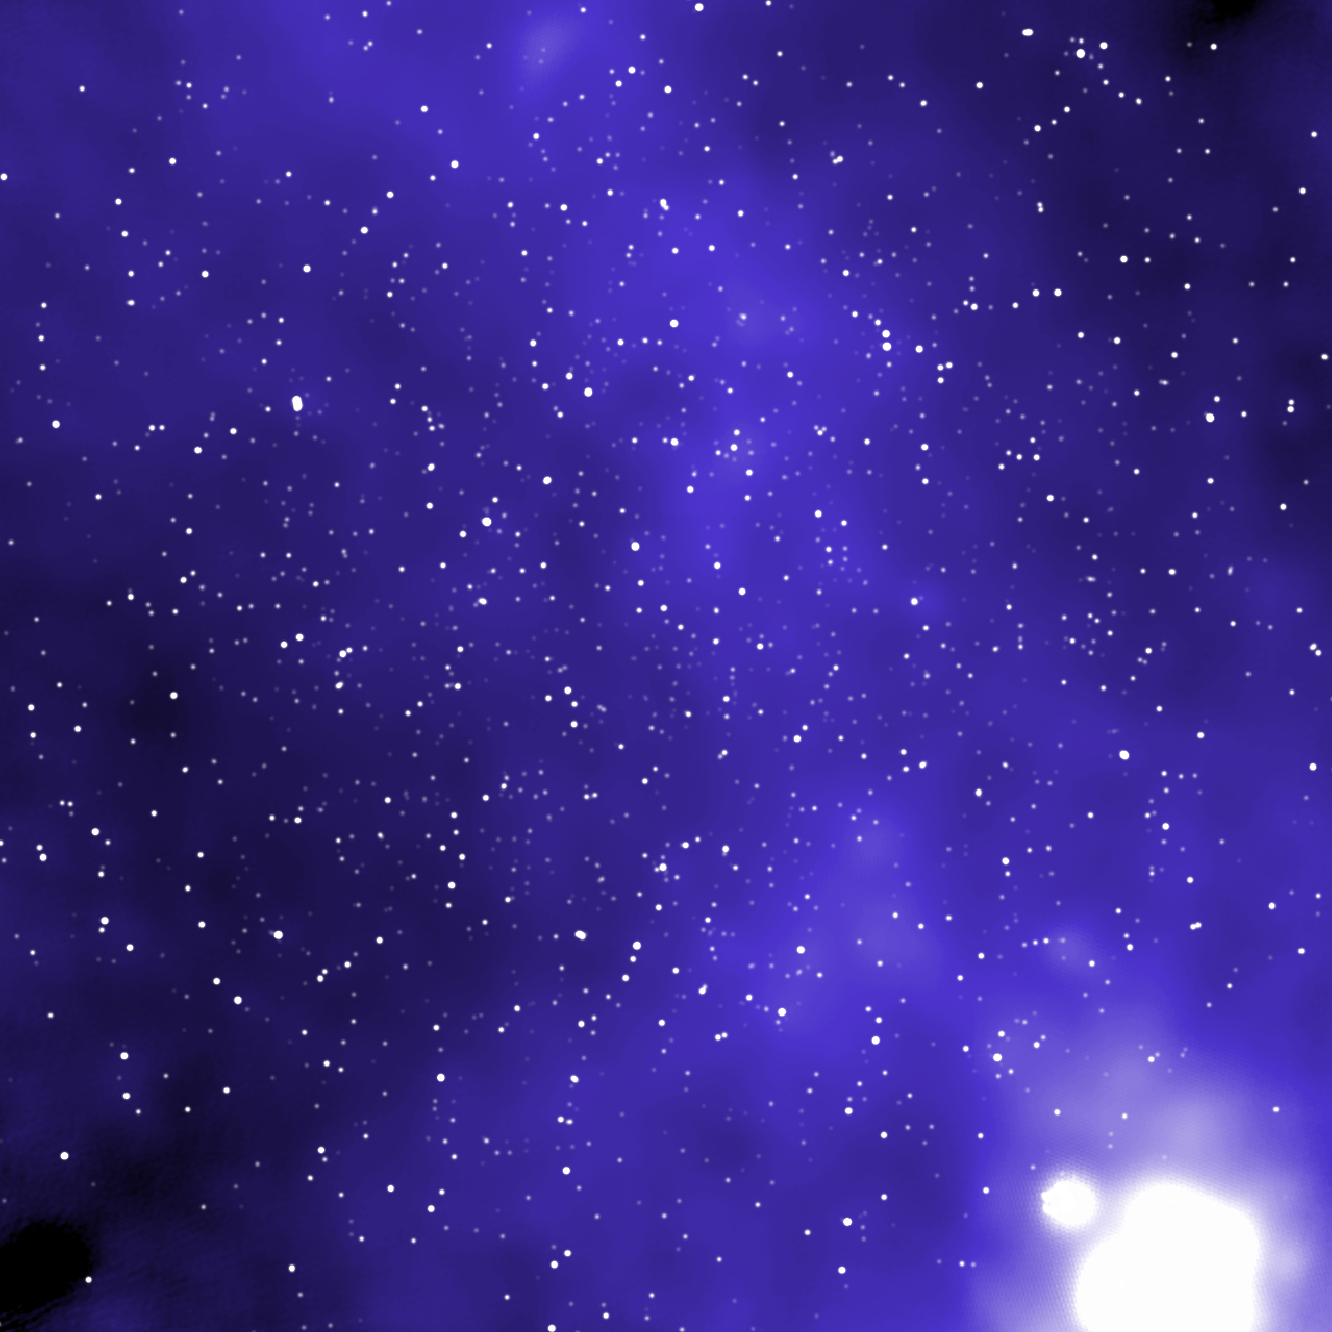
\includegraphics[width=6.5in]{plots/MWApretty.png} 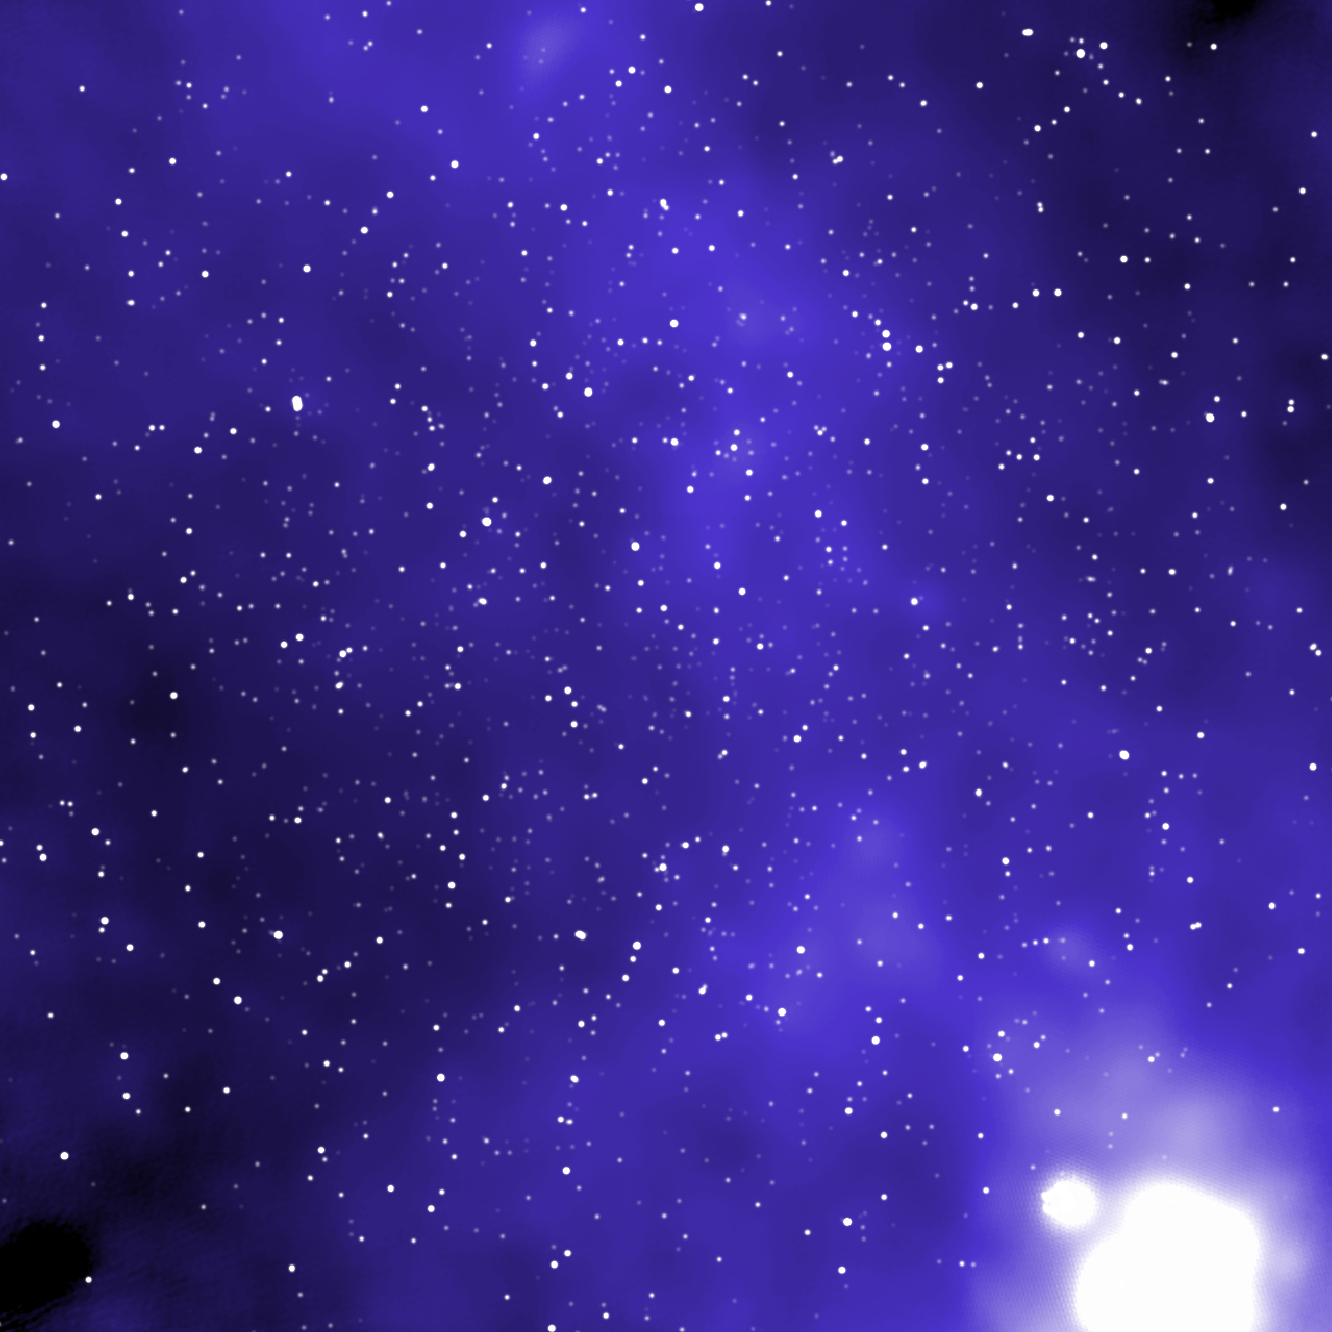
\includegraphics[width=3.6
%in]{plots/MWApretty.png}
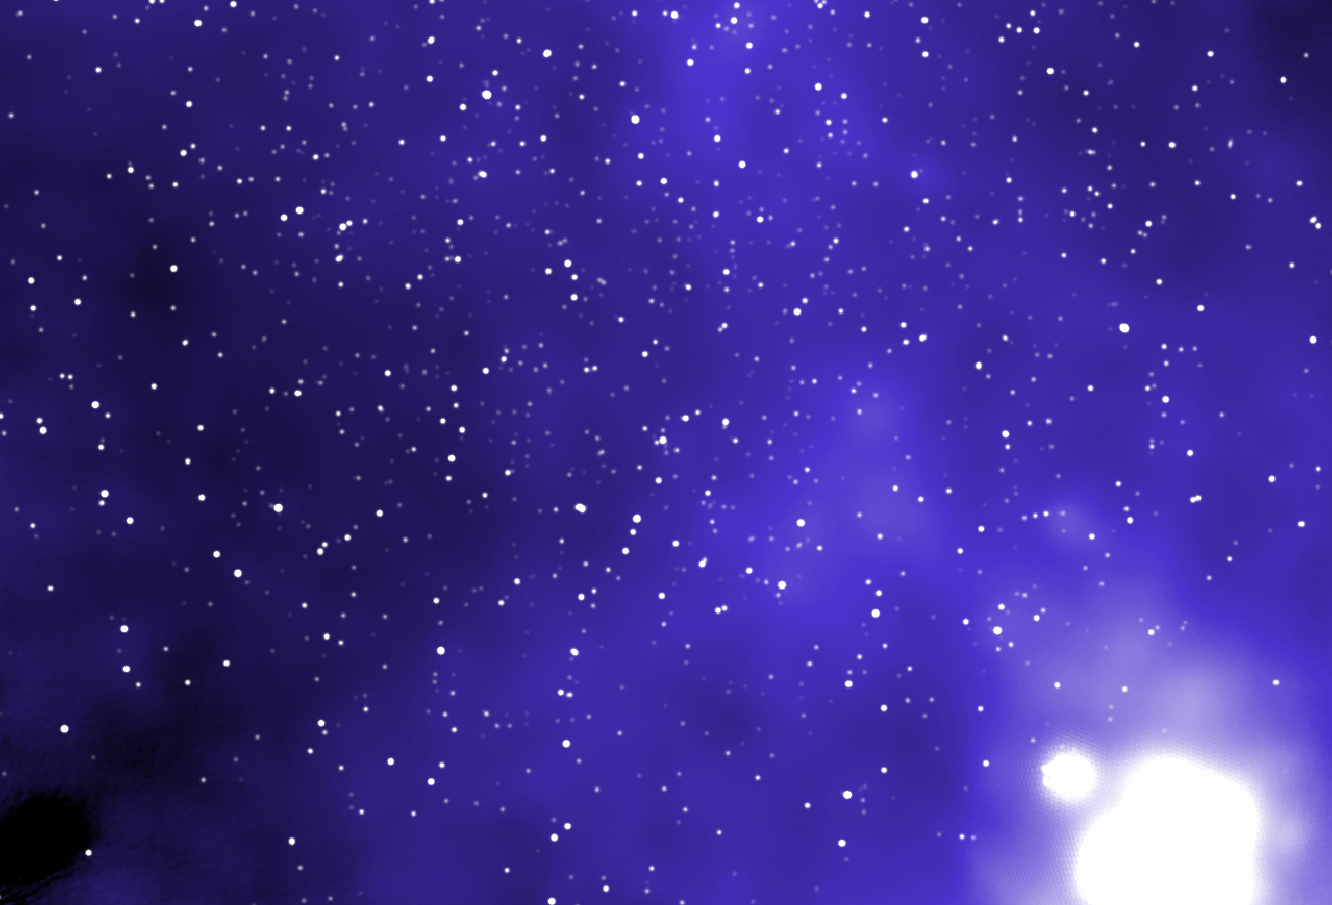
\includegraphics[height=2.3in]{plots/MWApretty_crop.png} % XXX replace with MWA pic from FoV fig
%\includegraphics[width=2.4 in]{plots/wedge_tall.png}
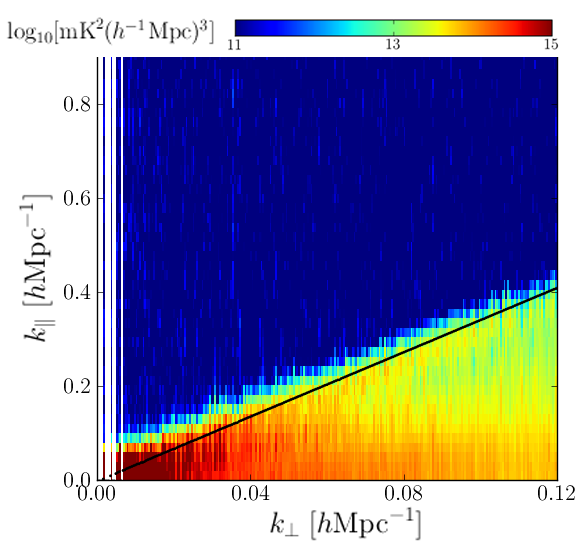
\includegraphics[height=2.3in]{plots/wedge_tall_wide.png} \caption{\small Left:
Foregrounds imaged on the MWA using FHD software.
This image spans $\sim$$30^{\circ}$ and
includes point-source and diffuse emission (the Vela and Puppis SNRs are in the
bottom-right). Imaging methods provide a key capability for reducing
polarization leakage and foreground systematics.  
Right: Foreground contamination in line-of-sight $\kpar$ vs.\ angular $\kperp$
as observed using PAPER \citep{pober_et_al2013}.
Foregrounds are bright within a ``wedge" (lower right) and then fall 
precipitously in the ``EoR window" (blue/black 
region), where measurements are thermal-noise limited.  The wedge's location can 
be estimated analytically (solid black line), but the foregrounds leak out by a margin 
dictated by the chromatic properties of both the foregrounds and the instrument.
%Bright foregrounds occupy
%a wedge (lower right) that extends beyond a fundamental analytic limit
%(solid black) by a margin dictated by the chromatic properties of the foregrounds
%and the instrument, and then falls precipitously
%in the EoR Window (blue
%region), where measurements are currently thermal noise limited. 
This insight has led to the
first meaningful constraints on EoR via 21~cm emission
\citep{parsons_et_al2013}.
}\label{fig:twoFGViews} \end{figure}



%i. describe arrays, state design driven by new understandings as delineated below (Fig)
% ARP: check, above % Parsons, Bowman

%ii. Using new techniqes, current best limits  (Fig)
% ARP: check, above % Parsons, Morales

%iii. what will happen in next 2 years: hopefully detection, but no more

%iv. LOFAR/MWA/PAPER 
% Carilli
% XXX ARP: I think paragraph below should really emphasize concrete limitations of 
% current experiments, and describe how HERA blows this wide open
%Three reionization path-finder array experiments are currently
%operational: LOFAR, MWA and PAPER. All three are designed to have the
%sensitivity to make the first statistical detection of the neutral
%IGM. However, the HI line experiment is very challenging due to
%foreground continuum emission some four orders of magnitude brighter
%than the expected line signal.  The three experiments offer very
%significant complementarity, with different intrinsic systematics and
%different approaches to foreground mitigation. We emphasize that, for
%such an important discovery, multiple approaches are critical in order
%to check and verify any claimed (likely low S/N) detection amidst the
%substantial systematic uncertainties. The first detection of
%the neutral IGM is not the end of reionization studies, just the 
%beginning. Recall that some four decades separated the first detection
%of the CMB from the first statistical characterization. 
%
%
%iv. HERA II: 'gauranteed' detection, full characterization, dark ages, imaging
%% Aguirre
%
%v. Move 'analysis' stuff here?

%%%MM:  I think the Challenges have been largely subsumed into the above section, at the level of detail we want to put in a proposal, so I've commented out this section. Just a thought.

%\section{Challenges} % 2 pages
%
%\subsection{Foregrounds}  % 1.5pages
%% Parsons, Morales
%
%
%i. relative intensities (Fig: Continuum from MWA)
%
%ii. Details on Delay Spectrum approach
%
%a. key: 3D k-space: show wedge and discuss. chromatic sidelobes with characteristic freq scale 
%set by baseline length
%
%b. analysis focuses on line-of-sight PS dimension
%
%c. work in EoR window.  different window levels, depending on effective horizon
%
%d. drives design to redundant array: helps calibration, add spectra coherently
%
%e. dictates geometry of antenna elements and other RF stuff. avoid standing waves of given length. 
%
%f. area: drives sensitivity as used in section 2
%
%g. some words about why compact, hex array 
%
%\subsection{Other Challenges} % 0.5 pages
%
%i. Interference: Karoo RFI plots  FIG 
%% Jacobs
%
%i. Polarization 
%% Moore, Aguirre
%% XXX ARP: I'm worried about this section.  In my mind, this is the one risk we
%% haven't truly retired yet.  We need to tread very carefuly if we bring this
%% up in depth.
%
%D. Ionosphere: 
%
%i. short baselines and narrowish FoV
%
%ii. direction dependent gains?



%  ___         _           
% |   \ ___ __(_)__ _ _ _  
% | |) / -_|_-< / _` | ' \ 
% |___/\___/__/_\__, |_||_|
%               |___/      

\section{HERA Project Design} % 8 pages

% XXX address this:
% the proposal would be more convincing as an
% "experiment" if there were more of a flow from a specific science goal, down to
% technical requirements, down to your implementation.  This would boost
% reviewer's confidence that you will achieve a specific stunning science result
% if the project is funded.  And I think it will save you a few pages of text
% because there is a lot of repetition about things like avoiding reflections
% which could be eliminated if explained clearly at the outset.  And some
% important things are never justified, like the area of the survey or the
% collecting area needed to accomplish the science. 

% XXX also mention HERA design philosophy of designing conservatively wrt foregrounds,
% based on known techniques,
% but supporting a battery of foreground mitigation techniques.

%\subsection{Lessons learned recap} % 0.5 page

% XXX possibly pull some of the sentences below for HERA Lessons section above.

%The HERA collaboration has made significant progress on multiple approaches in dealing with
%foregrounds.
%Based on a ``delay-spectrum'' understanding of
%the mechanism for how instrumental responses modulate foregrounds on
%spectral scales of cosmological interest \citep{parsons_et_al2012b},
%PAPER has optimized its instrument to focus on regions in Fourier
%space that have weak coupling to foregrounds caused by the
%interferometer.  These regions are determined both by chromatic
%instrumental responses and by the inherent frequency structure of the
%foregrounds.  An `EoR window' has been identified in the Fourier
%(wavenumber) space of spectral and angular power spectra that is
%inherently free of continuum emission, without explicit continuum
%subtraction in either the image or spectral domain \citep{pober_et_al2013,morales_et_al2012,Datta_2010}
%This window allows for continuum
%`avoidance' rather than subtraction. Observations based on this new
%approach have already demonstrated that the extremely stringent level
%of foreground suppression needed to access the 21~cm signal is largely
%in hand (as shown in Figure \ref{fig:pk_k3pk}), with upper limits
%that are beginning to rule out cold reionization scenarios \citep{parsons_et_al2013}.

This HERA proposal targets a 331-element array that incorporates
our proven foreground avoidance techniques while improving
dramatically the sensitivity relative to current experiments.  With a
new understanding of how antenna size and separation affect
sensitivity and foreground isolation, it has become evident a revision
of the PAPER antenna design can yield up to 20 times the sensitivity
per element without substantially degrading foreground isolation.
Where PAPER's elements lack collecting area and are smaller than
strictly required for foreground isolation, and the majority of MWA
and LOFAR elements are spaced too widely to avoid foregrounds,
HERA-331 employs an extremely compact array of 14-m parabolic dishes
with PAPER-style dipole feeds (see Figure \ref{fig:hera_dish}).  The dishes
are placed in a compact hexagonal configuration of 331 dishes supplemented by 18 outrigger dishes to achieve dense and
highly-redundant $uv$-sampling (see Figures \ref{fig:uv_coverage} and \ref{fig:config_optics}).  The dishes have a short (4.5m) focal height to limit the
path length of reflections, whose time-delay gives rise to chromatic
instrumental systematics.

\begin{figure}[!ht]
\centering
		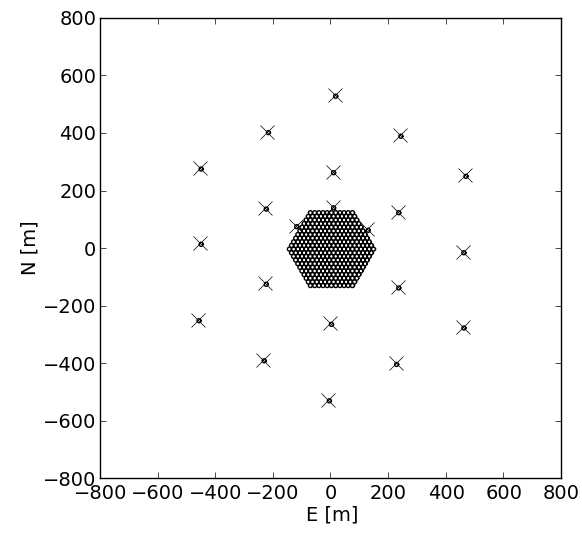
\includegraphics[width=0.45\textwidth]{plots/HERA_331_pos.png}
		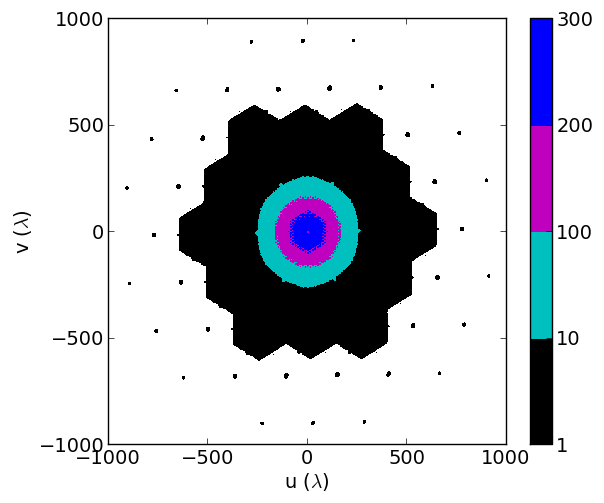
\includegraphics[width=0.45\textwidth]{plots/HERA_331_uv_clipped.png}
\caption{Left: Configuration of HERA-331, with 331 dishes in a maximally-dense hexagonal core and 18 outrigger dishes.  Right: The resulting $uv$-coverage is fully-sampled to $\sim 200\lambda$ [XXX: is this the ``official" figure to quote?]}
\label{fig:uv_coverage}
\end{figure}

% AAARRGGHH!
%\begin{figure}[!ht]
%\centering
%	\begin{subfigure}[b]{0.46\textwidth}
%		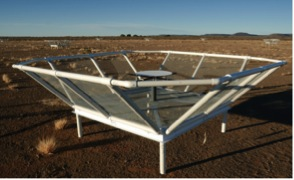
\includegraphics[width=\textwidth]{plots/paper_element.jpg}
%		\caption{The PAPER element (provides a clean instrumental response as a function
%		of frequency \citep{parsons_et_al2010,parsons_et_al2012b}, which is crucial to
%		the foreground isolation shown in Figure \ref{fig:eor_pspec}.}
%	\end{subfigure}
%	\quad
%	\begin{subfigure}[b]{0.46\textwidth}
%		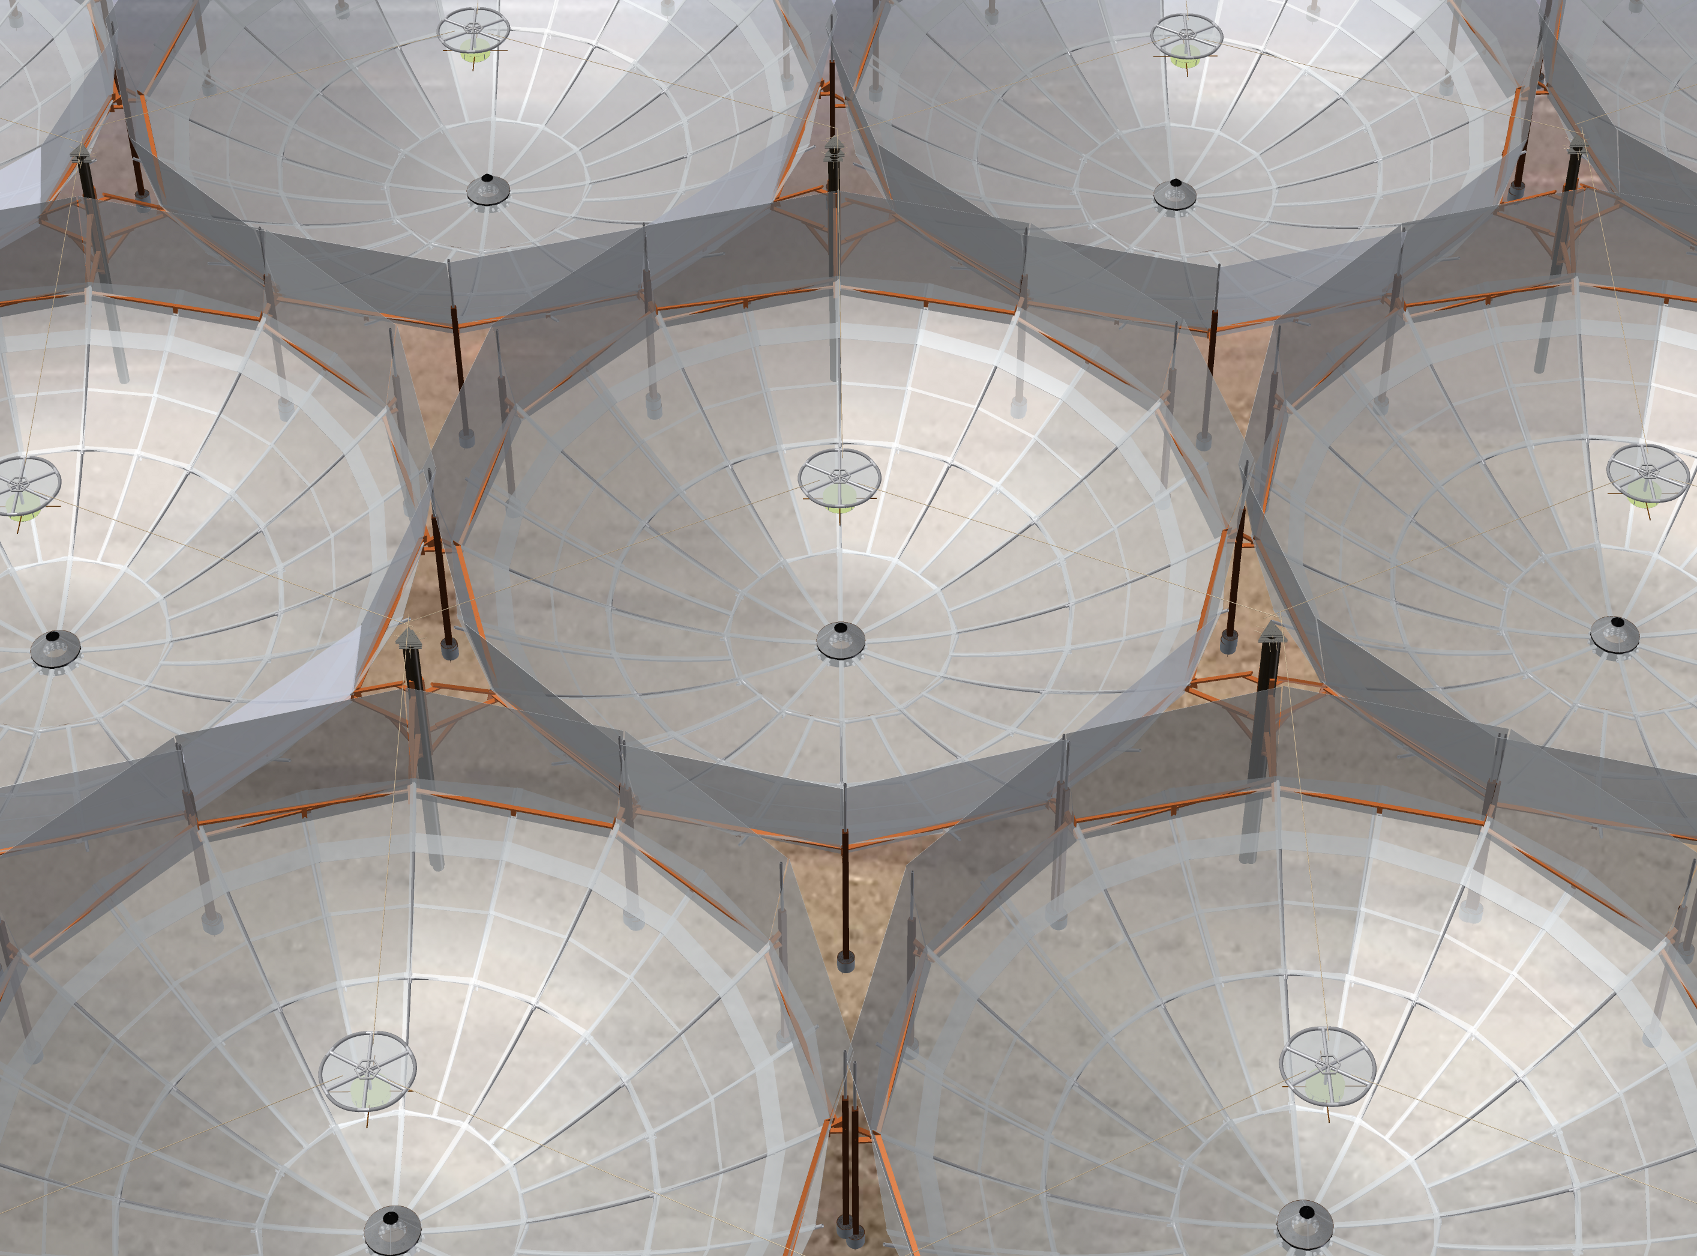
\includegraphics[height=1.75in]{plots/hera_dish.png}
%		\caption{A 14m dish designed around the feed dramatically improves sensitivity while
%		constraining the path length and amplitude of reflections to ensure that foreground 
%		isolation is not substantially degraded.}
%	\end{subfigure}
%\caption{PAPER and HERA elements}
%\label{fig:hera_dish}
%\end{figure}

The size of HERA-331 dishes optimizes cost for a fixed sensitivity and
level of foreground isolation.  The associated reduction in the number
of antenna elements to achieve a given collecting area, combined with
the fact that these dishes have no moving parts, are built from
inexpensive materials, and follow a simple construction that can be
contracted locally, makes the cost of building HERA-331 substantially
cheaper than was anticipated in the roadmap submitted to \nwnh\ for this
stage of the program.   

HERA leverages the technical heritage of PAPER, MWA and of CASPER\footnote{Collaboration for Astronomical
Signal Processing and Electronics Research, a Berkeley-initiated worldwide open source community that is
developing boards, firmware and software for the astronomical community} and incorporates a
phased implementation to mitigate against risk.  The system, technology and phased approach is discussed below
in more detail.

\vspace{-0.25in}
\subsection{Instrument Design}
\vspace{-6pt}
\label{InstDes}
The HERA instrument design is very straightforward.  The element
itself is a fixed zenith-pointing 14-meter segmented prime-focus paraboloid with a high screen
to minimize cross-talk between elements (which are spaced 14.3 meters on a
hexagonal grid).   The $f/D$ of
the paraboloid is 0.32, so that the focal length, $f$, is less than 5 meters to meet the 
standing wave specification at the delays of interest of more than 60 dB of attenuation at delays 
greater than 50 ns.


The active feed sends back the entire dual-polarization analog bandwidth on standard
coaxial cable to an aggregation point called a ``node'', which services 
about 15 antennas.  This cable length is kept short (35-m) to keep any standing
wave contamination outside of the delay-space of interest for power spectrum
measurements.  The node amplifies, filters, digitizes and transmits the signal data stream
back to the central processing location (the Karoo Array Processing Building - KAPB).
Figure \ref{fig:blockDiagram} shows a block diagram of the system.

\begin{figure}[h]
\centering
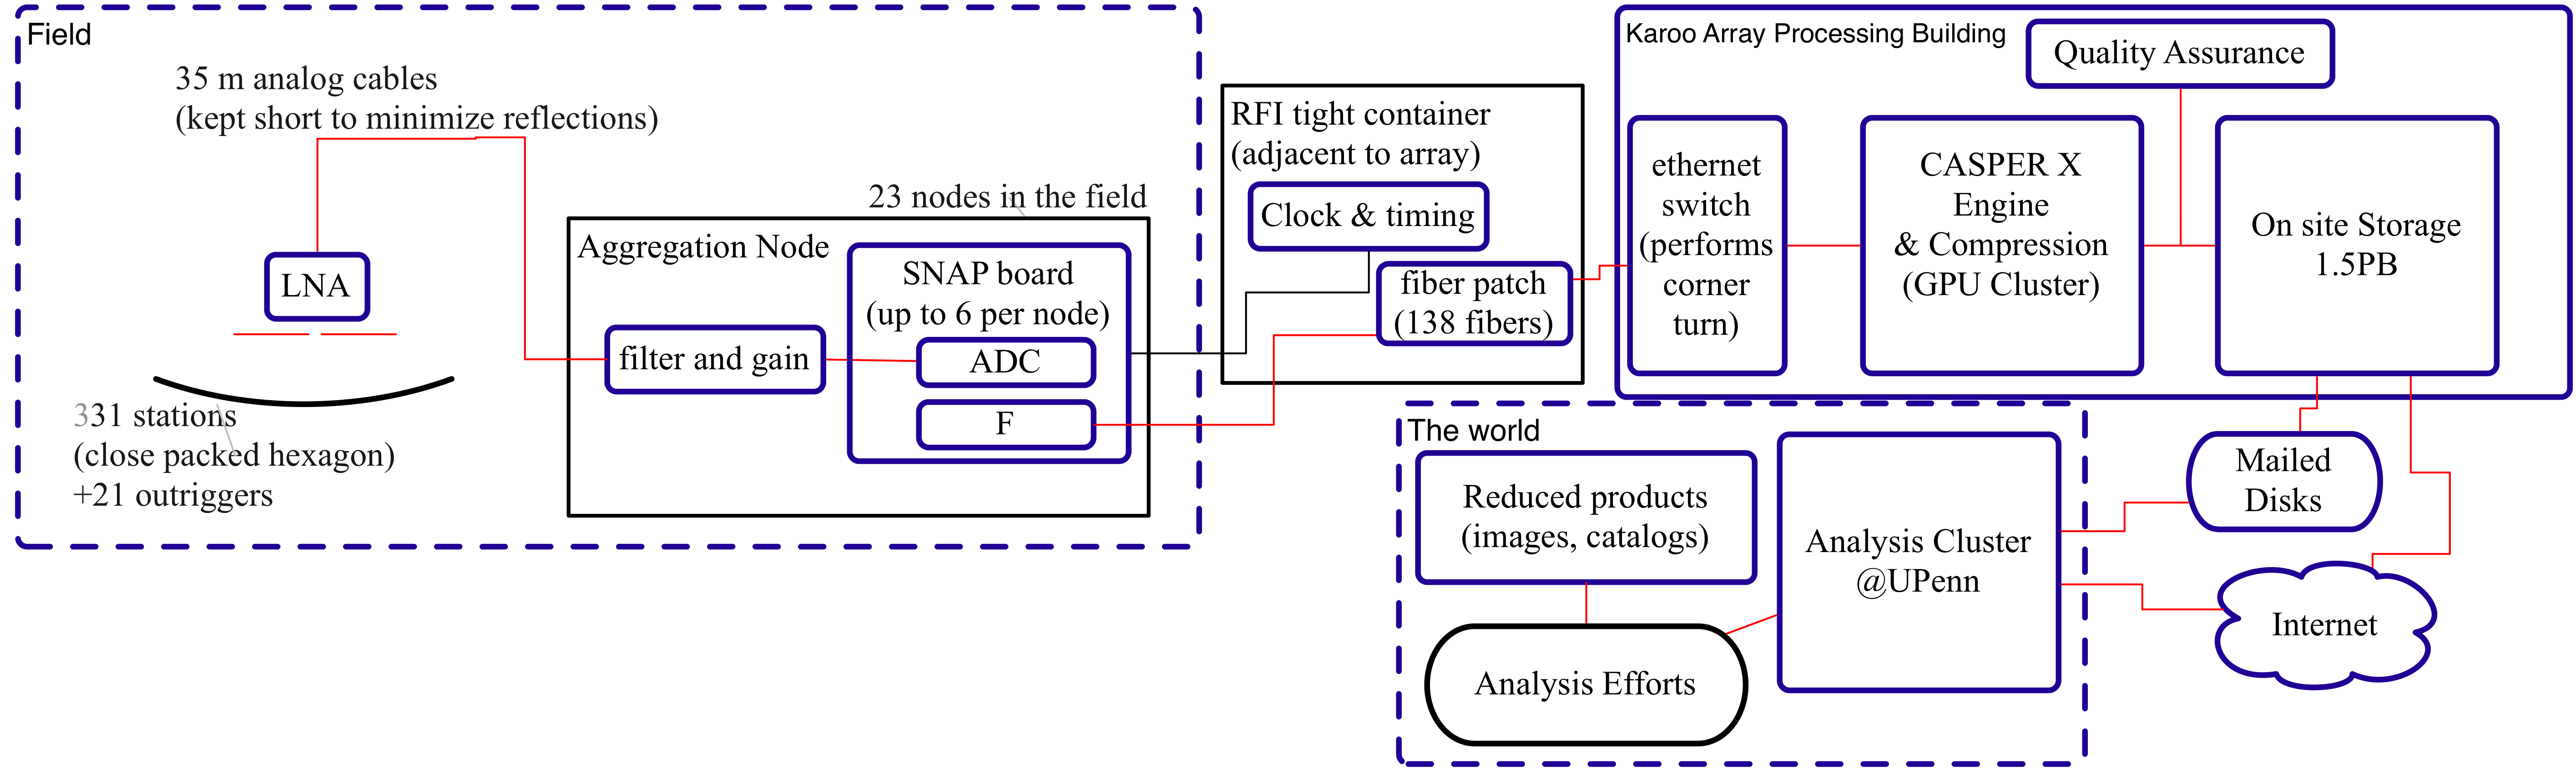
\includegraphics[width=\textwidth]{plots/Engineering/HERA_high_level_block_diagram.png}
\caption{Block diagram of the HERA system.}
\label{fig:blockDiagram} 
\end{figure}

\vspace{-0.25in}
\subsubsection{Element and Configuration}
\vspace{-6pt}


The element is a fixed zenith-pointed mount, which dramatically simplifies design and
operation. Cost is a key design constraint for this experiment, which has components
for construction materials, assembly in a remote area, and operation over its
lifetime. As an experiment, the design lifetime is 6 years, which helps constrain
costs relative to a long-lived facility. For a field-deployed instrument, one needs
to define limited well-constrained reference points for accuracy in construction. The
proper installation procedure is therefore critical in construction. The elements are
also nearly abutting one another, which allows for sharing of physical support
infrastructure.

Given the delay-spectrum technique developed for 21~cm EoR science, it is important
to ensure that internal reflections within the antenna structure are at a low enough
level at delay values where the array has sensitivity to the EOR power spectrum. That
is, we don't want reflections that will modulate foregrounds to corrupt scales
corresponding to the desired $\kpar$, scattering foreground power into the EoR
window. Recent work characterizing foregrounds suggests that the spectral structure
of foregrounds observed with baseline separations of $8\lambda \approx 15$m are
well-behaved to current limits \citep{pober_et_al2013b,parsons_et_al2013}. This sets the upper limit
for the dish diameter at about 15m. However, this requirement also sets restrictions
on the focal length of the dish since the primary resonances in the dish will be the
standing waves that arise between the primary reflector and the antenna feed, caused
by imperfect impedance matches of the feed electronics and free space, as well as by
the presence of any metallic structure in the area.

Many competing factors set the area of the collecting element. Among them are
sensitivity, cost, minimum baseline, efficiency and delay values of internal
reflections, as just mentioned. Using the derived sensitivity for a redundant array
\citep{parsons_et_al2012a} and a reasonably complete costing model, one can compute
the cost/performance for a fixed sensitivity as a function of diameter. 
%Figure \ref{fig:nvsd} shows this function normalized to a 14-meter antenna, indicating a
The cost function normalized to a 14-meter antenna shows a
fairly broad minimum extending from about 14 to 22 meters. 
%Arrows indicate the
%direction of increasing systematics and delay-space contamination. 
Within this range,
smaller elements are preferred because of increased field of view and lower
timescales for delay-space contamination arising from reflections.

% ARP: lack room for this figure.
%\begin{figure}[h]
%	\centering
%	\begin{subfigure}[b]{0.46\textwidth}
%		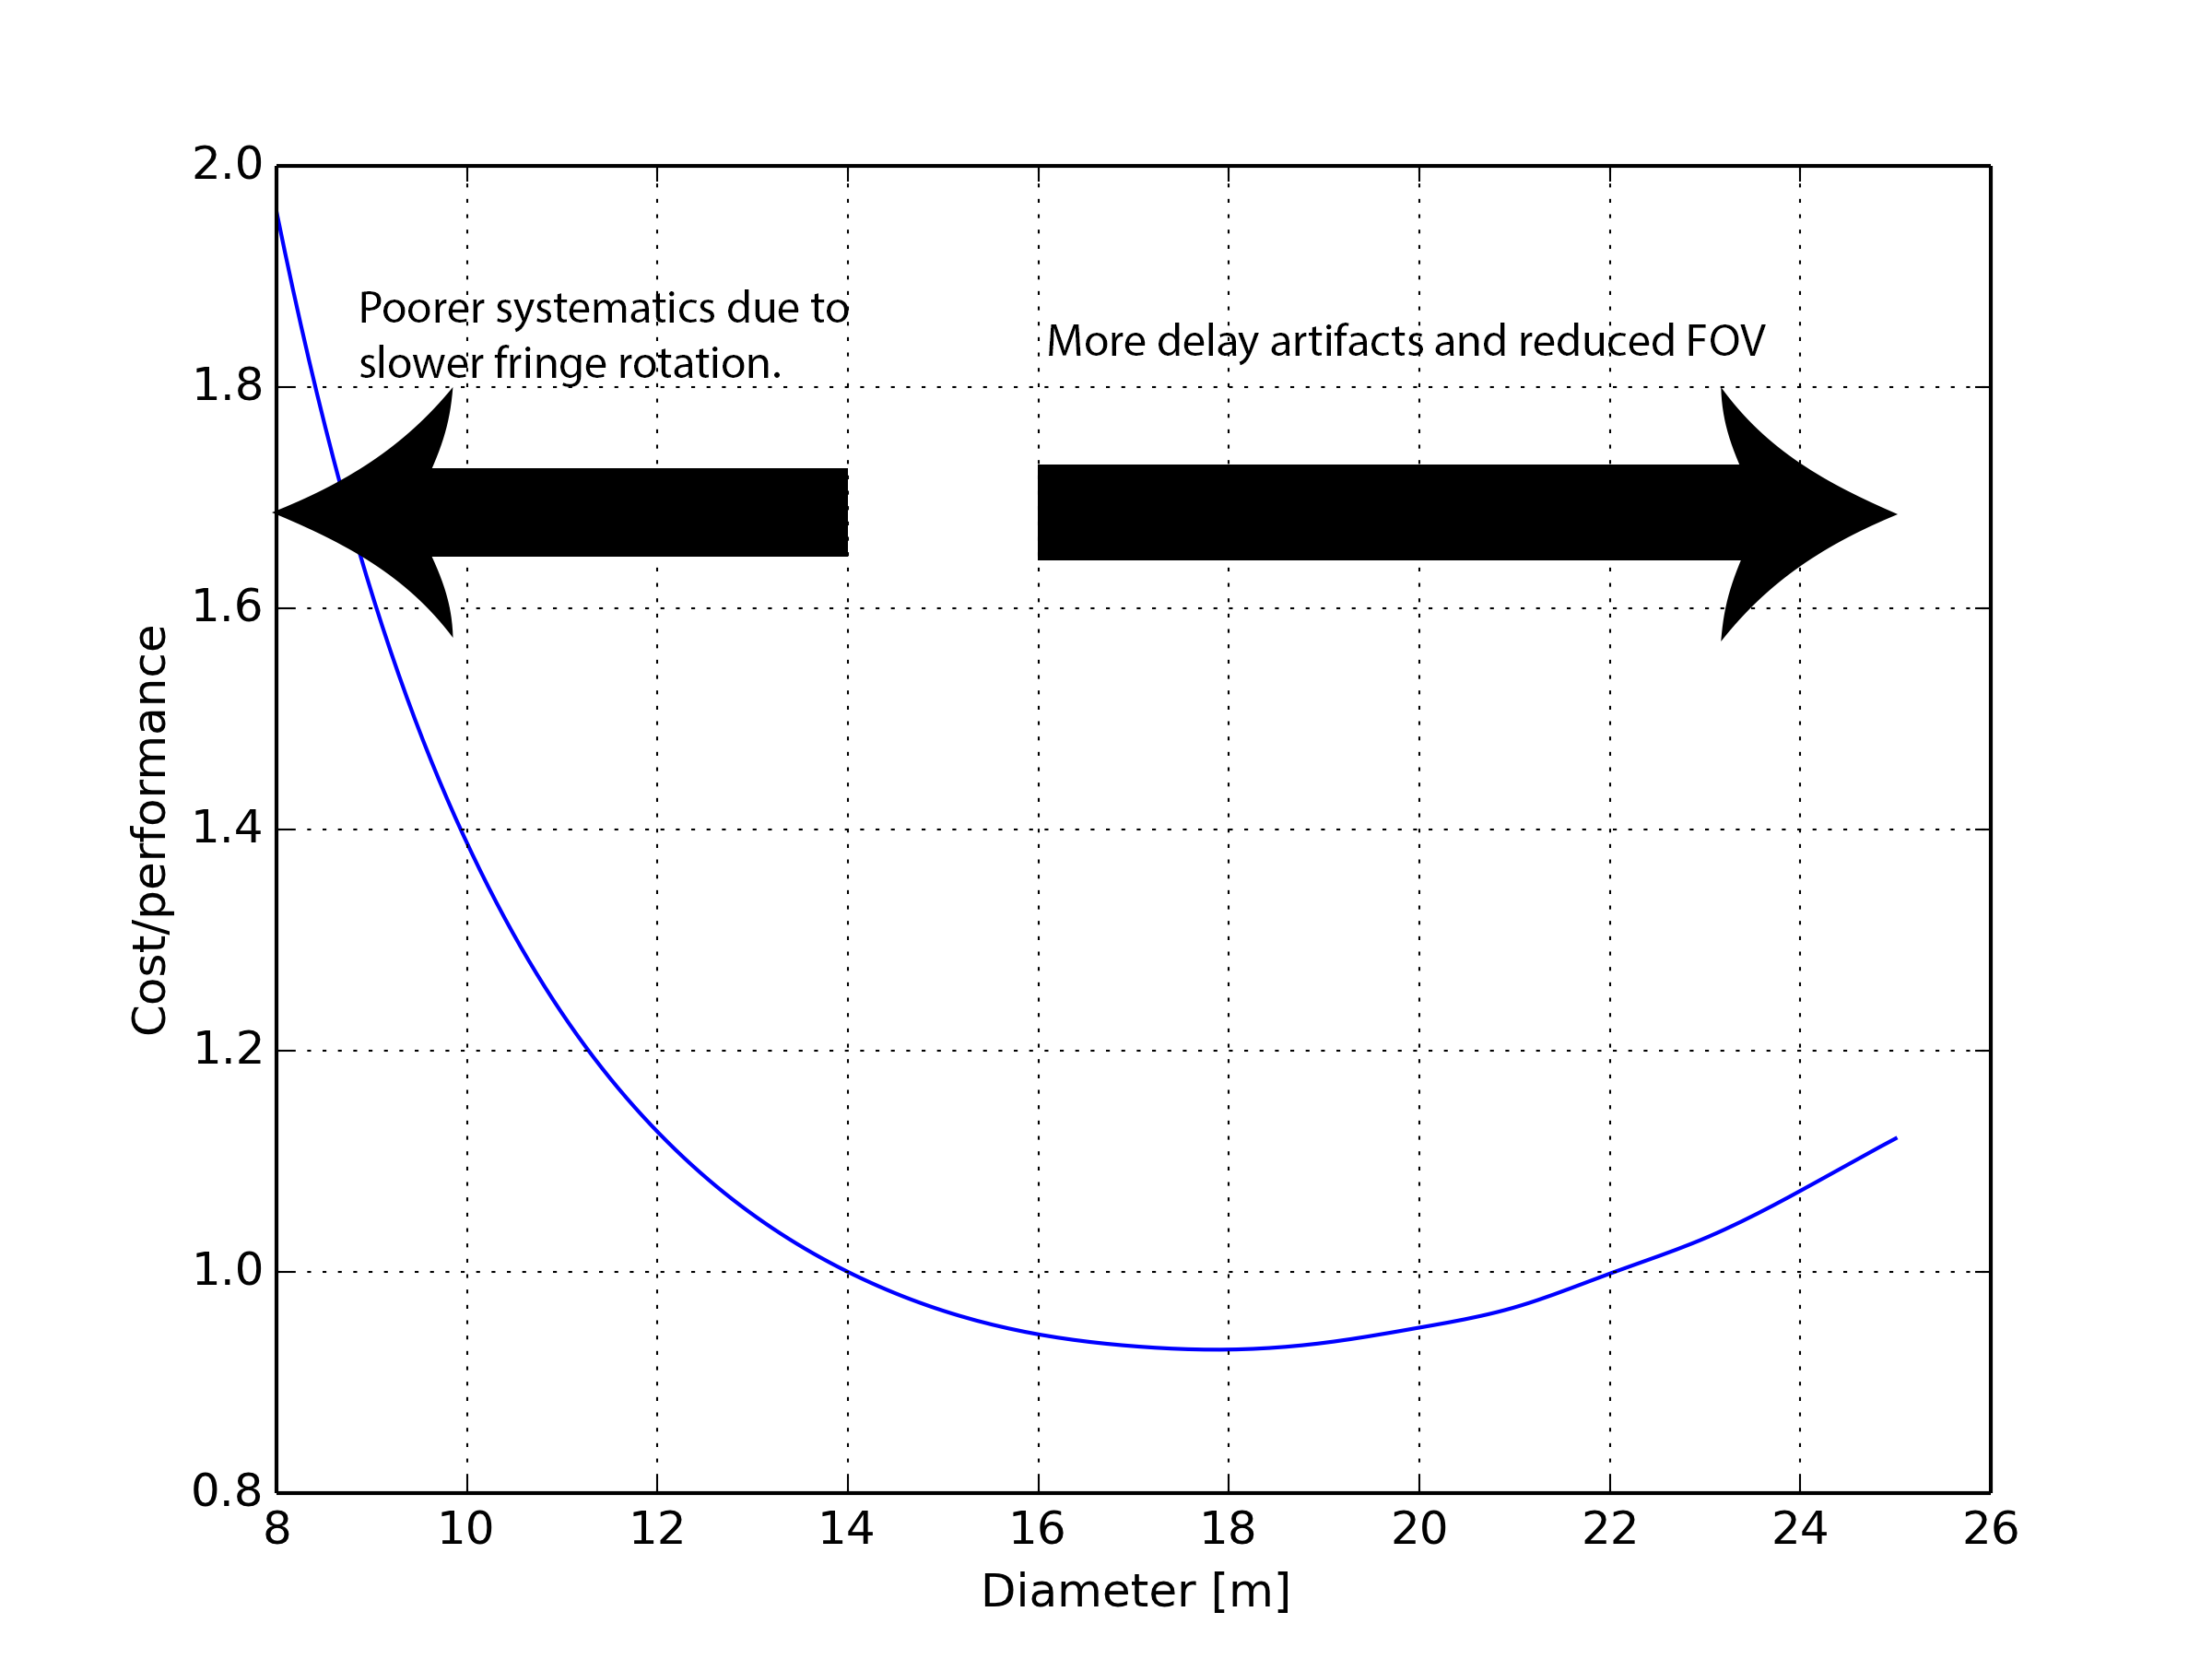
\includegraphics[width=0.9\textwidth]{plots/Engineering/nvsd.png}
%		\caption{Costing model for a fixed sensitivity and varying the diameter.   The arrows indicate the regions of 
%				increasing systematics and delay-space contamination.}
%		\label{fig:nvsd} 
%	\end{subfigure}
%	\quad
%	\begin{subfigure}[b]{0.46\textwidth}
%		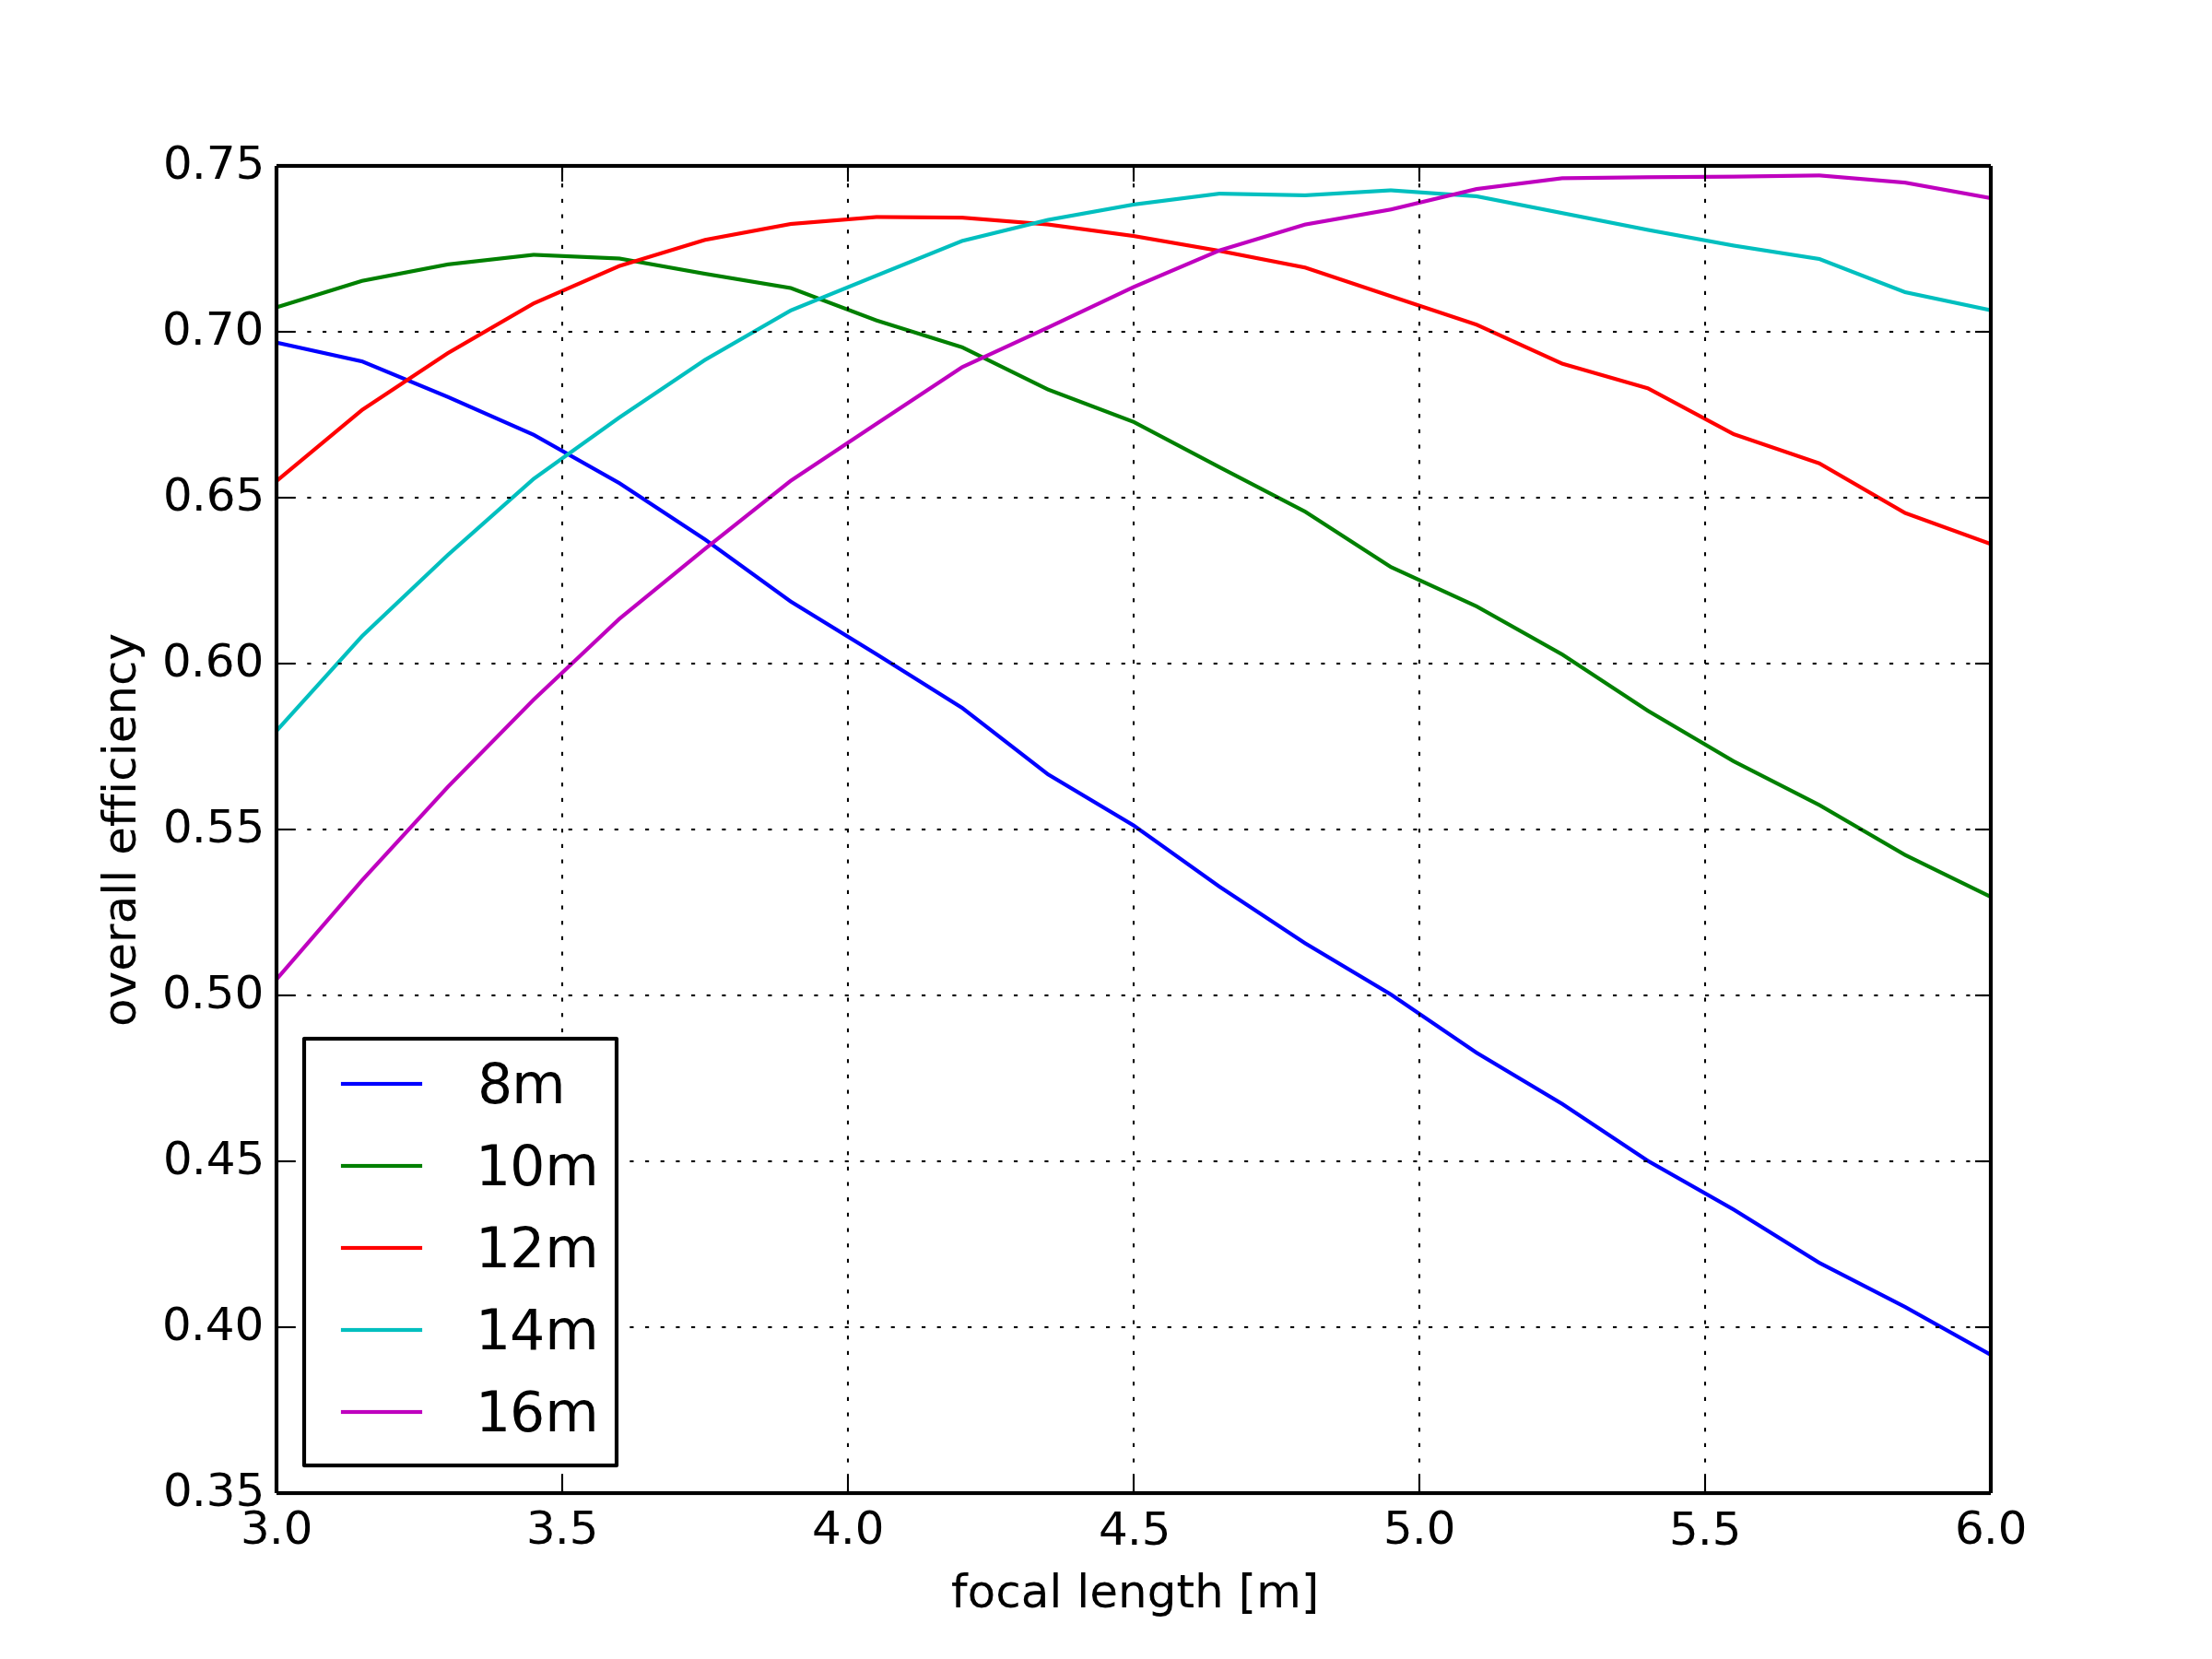
\includegraphics[width=0.8\textwidth]{plots/Engineering/focalEff.png}
%		\caption{Analytical model efficiency of a parabolic element as a function of focal height and diameter.   The delay 
%				contamination specification is $f<5$m.}
%		\label{fig:disheffic}
%	\end{subfigure}
%	\caption{Cost and performance variational analysis data for the element.}
%\end{figure}

% FOLLOWING SEEMS TOO DETAILED FOR A PROPOSAL
%To distinguish between measured sky delays and instrumental-induced delays at a required threshold ($R_T$) dB, 
%we need sufficient attenuation of the reflected signals at a given focal length ($f$) at a specified delay ($\tau_{d}$).  Assuming a conservative simple model that the magnitude of the reflection is attenuated by $A$ dB at each reflection 
%we see that for a delay length limit of $\delta_{d}=c\tau_{d}$ and focal length $f$,  the required focal length is
%
%\begin{equation}
%f < \left(\frac{A}{R_T}\right)\delta_d.
%\end{equation}
%
%Using nominal values of $R_T$ =  60dB (an order of
%magnitude below where EoR is predicted to be below foregrounds) at delays
%corresponding to the time it takes travel 15m and a net attenuation of 20 dB per reflection, 
%we find that the focal length should be less than about 5 m.  Free-space loss effects would 
%increase that value, loosening the constraint.
%DETAILEND

To maximize sensitivity, we wish to maximize the efficiency of the
HERA element, while still thresholding the delays at which reflections couple
back into the feeds. The design for the proposed HERA element is set
at $14~m$-diameter dish with a focal height of $4.5$~m, which currently gives us
good total efficiency %(see Fig \ref{fig:disheffic}) 
while staying within the delay-response constraint. 
%Analytical models of the beam pattern are shown in Figure \ref{fig:beam}.
Full electromagnetic modeling will be coupled with 
physical measurements of the prototype to validate and refine the element.

%In addition to the constraints given by the element itself, the HERA element size is
%also influenced by the location of the ``knee'' in the EoR power spectrum \citep{lidz_et_al2008}
%The EoR power spectrum has an upward slope for low $k$-modes which levels off
%around $k=0.15 h$/Mpc %(see fig blah). 
%Working inside this $k$-mode would be beneficial due to the fact foregrounds are
%less problematic. This poses a problem because without knowing the
%width of our foregrounds, we can't say for sure which $k$-modes (in the power
%spectrum) are corrupted. This uncertainty, coupled with increasing systematic affects for shorter 
%baselines (hence smaller diameters), favors larger diameter antennas.

%% ARP: no room for this figure.
%\begin{figure}[h]
%	\centering
%	\begin{subfigure}[b]{0.46\textwidth}
%		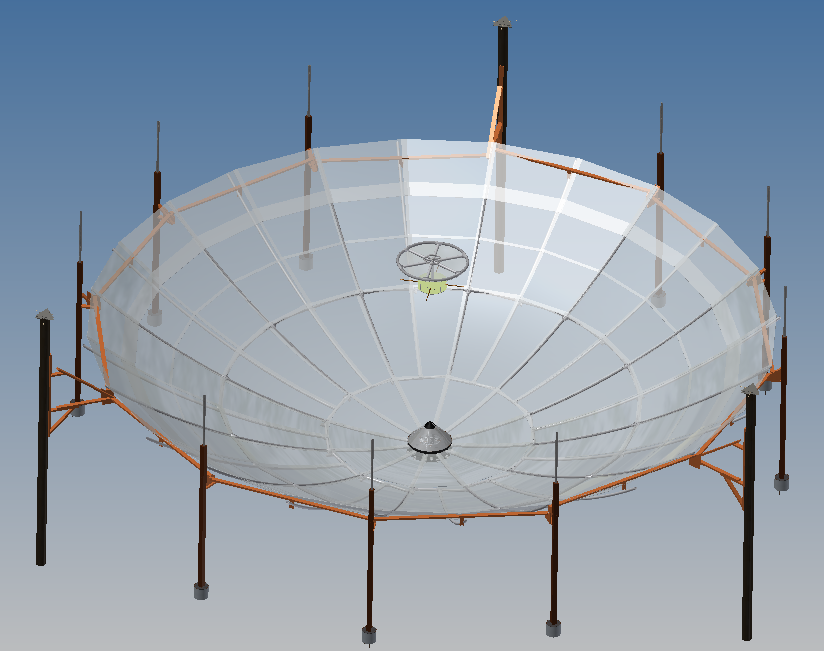
\includegraphics[width=0.85\textwidth]{plots/dish.png}
%		\caption{CAD model of 14m dish with screening and some supports removed to show detail.}
%		\label{fig:dish} 
%	\end{subfigure}
%\quad
%	\begin{subfigure}[b]{0.46\textwidth}
%		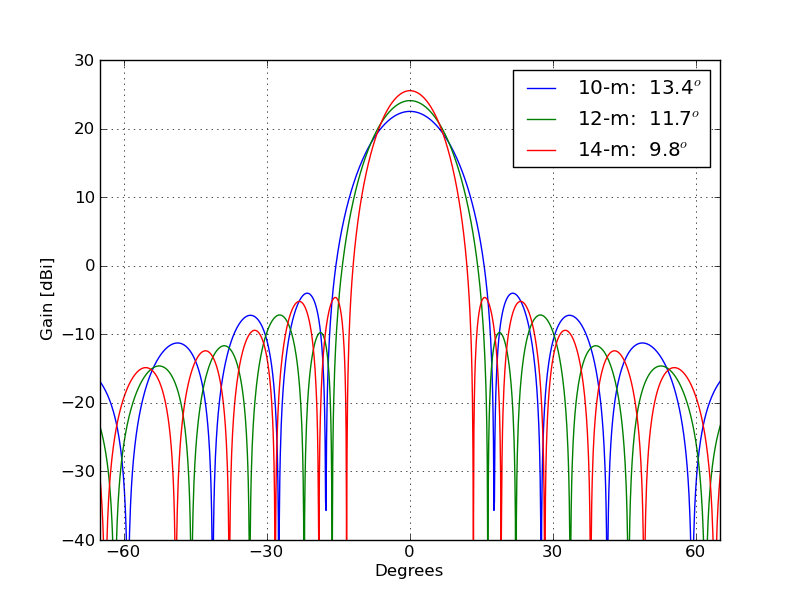
\includegraphics[width=\textwidth]{plots/Engineering/hera_beam.png}
%		\caption{Analytical model beam patterns at 10m, 12m and 14m.}
%		\label{fig:beam} 
%	\end{subfigure}
%	\caption{HERA element and beam pattern.}
%\end{figure}

%The $k$-mode for a $14m$ baseline is $k = 0.023$, given by $k_{H} =
%\frac{B}{c}\frac{dk}{d\eta}$, where $B$ is the length of the baseline, 14m in
%our case, $c$ is the speed of light, and $\frac{dk}{d\eta}$ is the cosmological
%transfer function from delays to $k$-modes. In addition, narcissistic
%reflections add into our $k$ budget as well. The $f$ and $D$ choices above provide a $k$ budget for
%foreground widths to be within $\Delta{k}\sim{0.1}$. Testing these hypothesis
%and again, finding a compromise between maximum sensitivity, foreground budget
%will be key to testing and constructing the required element. Foreground width constraints
%are still an area of active research \citep{pober_et_al2013}.

The core defining elements in this design are the central hub and three tall support poles.  Three intermediate 
support posts are installed between each pair of poles.  A 2$^{\prime\prime}$ PVC spar of 24.1$^{\prime}$ 
terminates at each pole and post.  These spars are supported at each end and one point in the middle at the 
proper height and angle.  The intervening PVC pipe essentially acts as a smoothing filter between those 
points, noting also that a beam with point loads attains nearly the quadratic shape desired.  The CAD model is 
shown in the right panel of Figure \ref{fig:hera_dish}.  

The tall ($\sim$ 7m) poles provide locational accuracy (in all three dimensions) for the overall array installation.  
Using conventional commercial pole-installation techniques the poles are installed first for the entire array.  
Note that every pole except for the edge poles are shared by three antennas.  A standard theodolite can 
then be used to mark a known level height on all three poles.  These locations are then used with tensioned 
lines to define the center of that element and the hub is positioned at that location using a jig.

The hub uses concentric commercially available ``sonotube'' forms (circular cardboard forms for concrete pillars) 
and PVC sleeves to hold the PVC spars and PVC supports.  The retaining holes may be accurately cut into 
the forms, sleeves installed and concrete poured to make a simple hub to the desired accuracy.  The jig holds 
the concentric rings in place and allows it to be centered by tensioned lines while the concrete is poured.  
When the concrete cures one can then transfer an accurate offset from the dish vertex back to the poles.
The intermediate posts are then located by the support sub-assemblies attached to the poles and posts along 
with the rim sub-assemblies.  These are positioned and a small pier is poured to locate them.  After spar support 
pieces are installed on the posts, the spars themselves and the metal cloth can be installed.

The feed is held off the three tall poles using tensioned lines to accurately locate it over the hub.  A precise 
length of kevlar rope holds the feed down to the hub at a precise focal point.  The RF cables follow the line 
down and out to the analog-to-digital converters and correlator.  

To minimize cross-talk, metal screens are strung between every pole/post, which go to the level of the feed.  
The dishes have a rim-to-rim spacing of 30cm to allow the screen to be slightly angled to minimize standing waves.

% XXX
%XXX There is nothing on the configuration yet.

\vspace{-0.25in}
\subsubsection{Signal Path}
\vspace{-6pt}
The signal path will utilize the front-end (feed and LNA, left panel of Figure \ref{fig:components})
and post-amplifier gain modules directly
from PAPER, although additional studies will be carried out to improve the feed
response below 100 MHz. The amplifier/baluns and post-amplifier modules already have
the ability to work over an extended lower end. The front-end amplifier has a low
noise figure with moderate gain, high dynamic range to tolerate RFI, unconditional
stability to ensure oscillation-free operation, well-matched impedance to both the
antenna and cable, well-understood temperature dependence, a mechanically rugged
mechanical design, low susceptibility to electrostatic discharge, low power
consumption, and low fabrication cost. It is housed in a metal enclosure affixed to
the antenna to form a very rugged, reliable, low-cost unit with excellent RF
performance \citep{parsons_et_al2010}.

% AAARRGGHH!
\begin{figure}[h]
	\centering
	%\begin{subfigure}[b]{0.3\textwidth}
		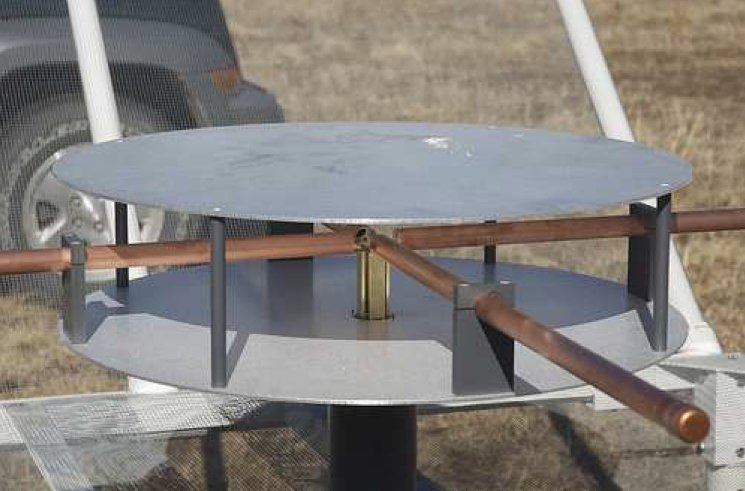
\includegraphics[width=0.3\textwidth]{plots/new_antenna_closeup.jpg}
		%\label{fig:element}
	%\end{subfigure}
	%\quad
	%\begin{subfigure}[b]{0.3\textwidth}
		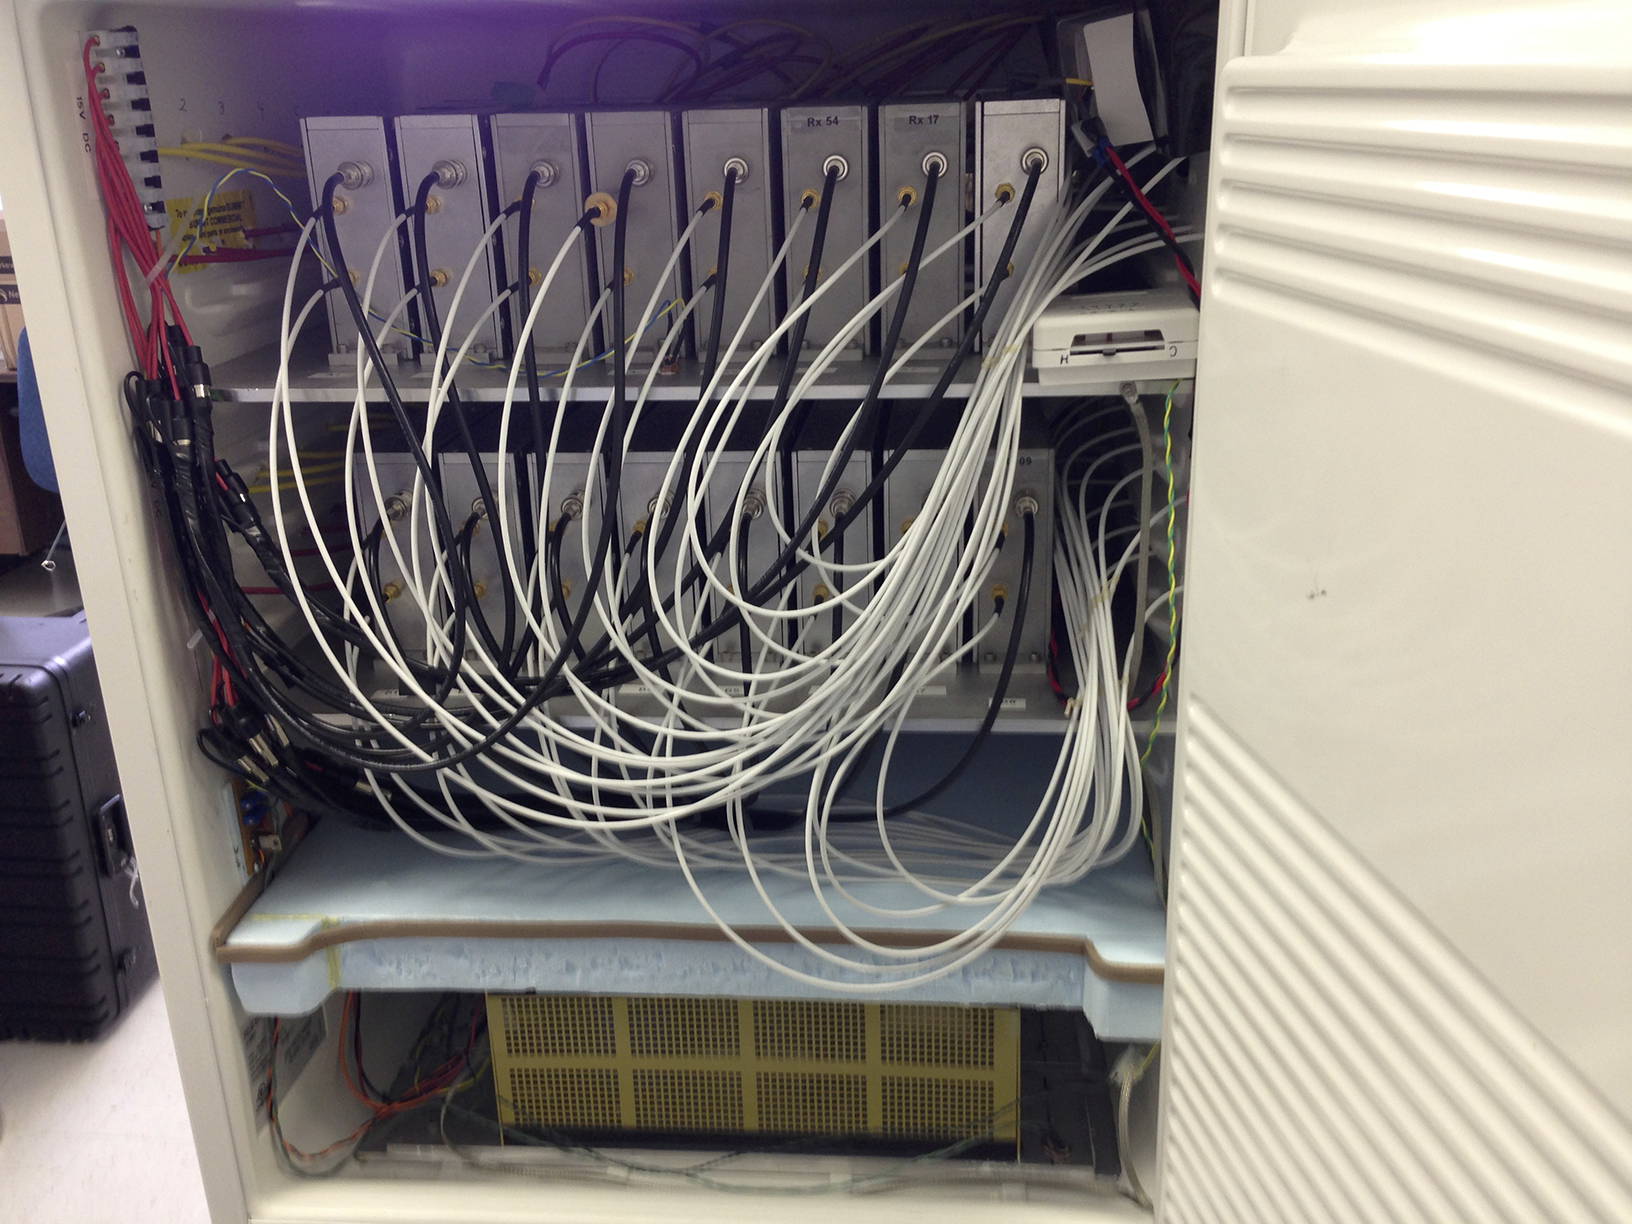
\includegraphics[width=0.3\textwidth]{plots/Engineering/recv_node.png}
		%\label{fig:recv_node} 
	%\end{subfigure}
	%\quad
	%\begin{subfigure}[b]{0.3\textwidth}
		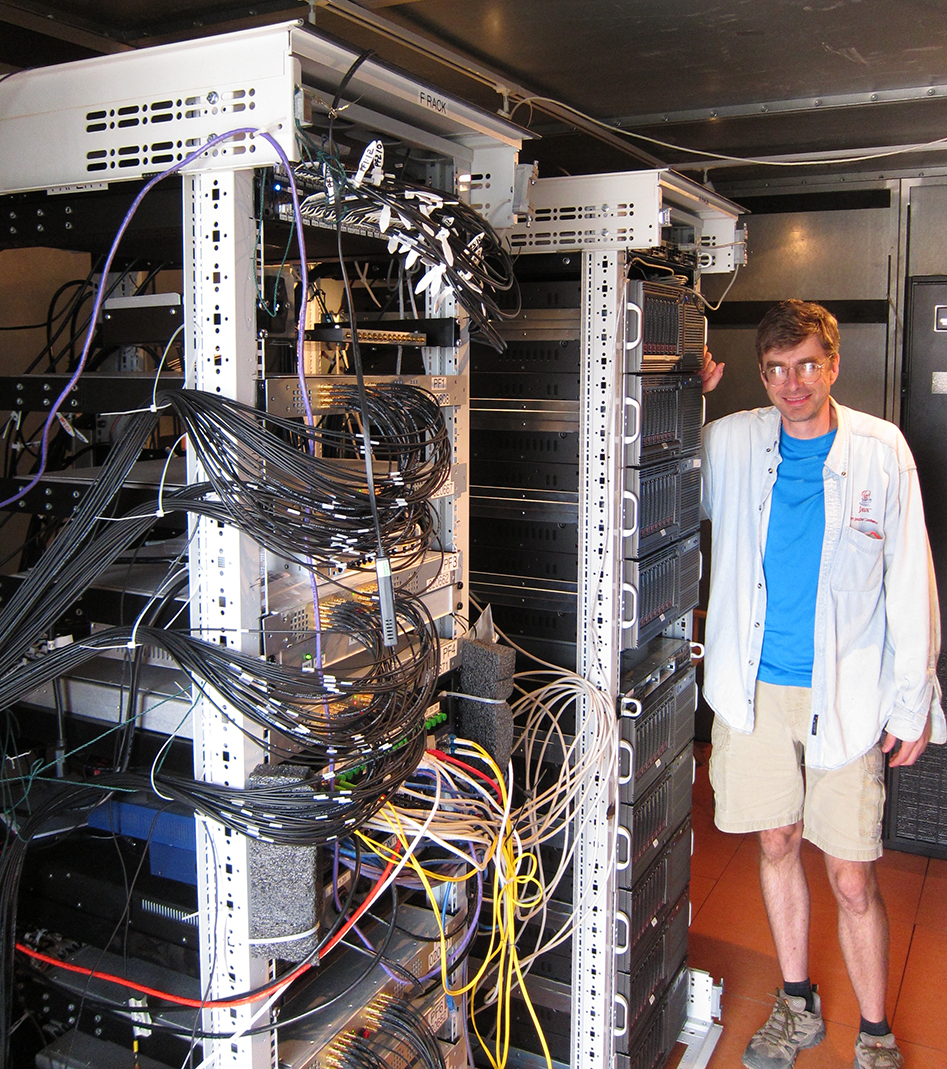
\includegraphics[width=0.24\textwidth]{plots/Engineering/digital.png}
		%\label{fig:digital} 
	%\end{subfigure}
	\caption{Photographs of existing instrument components to be used in the HERA design.
    Left: the PAPER antenna positioned above the trough reflector.
    Center: Receiver modules in a node refrigerator.
    Right: Digital equipment (ADC/correlator) in container.}\label{fig:components}
\end{figure}

The signal is transported to the node via a 35-meter run of 50 $\Omega$ coaxial
cables. It will terminate on a bulkhead plate on the face of the RFI-tight and
air-conditioned node. Inside, dual-channel post-amplifier modules (PAMs) (Fig.
\ref{fig:components}, center) amplify and band-limit the signal. Inside the RFI-tight node,
the PAMs themselves are housed in RF-shielded boxes.

A new board called the Smart Network ADC Processor (SNAP) board, to be incorporated 
into the CASPER suite of hardware and firmware, is currently in layout at NRAO.  SNAP
takes the output from the PAMs, digitizes and channelizes it before putting it on optical fiber
for transmission to the Karoo Array Processing Building.


%\subsubsection{Analog System}
%ii. 14m elements + broad band (active) dipole feed
% de Boer, Bradley

\subsubsection{Digital System}

Digital signal processing (DSP) electronics --- particularly the digital correlator ---
have historically been one of the most complex and expensive aspects of any radio interferometer.
Correlators have commonly been
developed independently for each project, with a substantial investment
of time and money to engineer
custom solutions for hardware, physical interconnect,
communication protocols, and control software. The complexity of such development
leads to lengthy incubation times and an
associated loss of timely scientific research. Furthermore, the large
engineering investments involved leave few resources
for upgrading systems that fall quickly into obsolescence as a result
of Moore's Law.

\begin{figure}[!ht]\centering
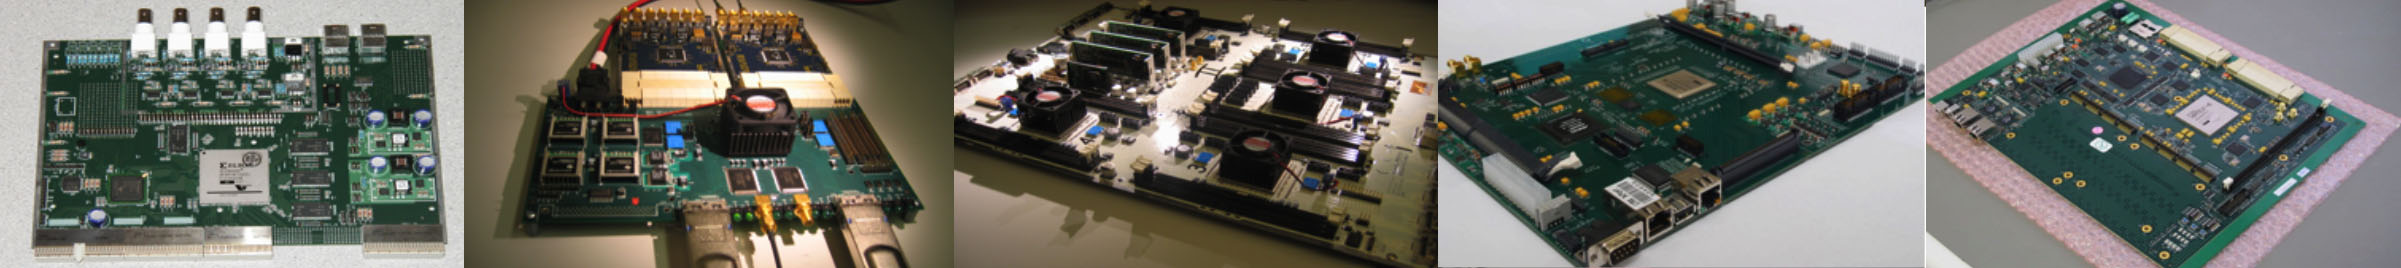
\includegraphics[width=6.5in]{plots/casper_boards.jpg}
\caption{
Five generations of CASPER technology (progressing left to right) have been used to rapidly
develop, test, and deploy DSP instrumentation for radio astronomy.  Correlators,
beam formers, and spectrometers all use a common set of hardware modules, along with a library
of parametrized DSP algorithms, that can be easily upgraded to incorporate new technology
\citep{parsons_et_al2006,parsons_et_al2008}.
}\label{fig:casper_boards}
\end{figure}

This is changing.  The Collaboration for Astronomy Signal Processing and Electronics Research
(CASPER; \citealt{parsons_et_al2006}) was founded seven years ago at Berkeley
by Werthimer and Parsons as a program 
to open-source and share the development of real-time signal processing engines for astronomy.
CASPER now has world-wide participation that is
transcending the radio astronomy community to include physics, engineering,
medical, and genomics research, with
over 500 members at 73 institutions, and, as illustrated in
Figure \ref{fig:casper_boards}, five generations of DSP hardware.
% XXX something about GPUs here?
As a result of the CASPER's cumulative body of open-source hardware designs, DSP libraries, instrument
architectures, and control software,
correlator development --- formerly the Achilles heel of building interferometers ---
is now widely viewed as a solved problem.  PAPER, on a modest budget, has developed and deployed new correlators
annually for five years running, each quadrupling the computational capacity of its predecessor.
HERA will continue this incremental development cycle, following the packet-switched
FX correlator architecture described in \citet{parsons_et_al2008} that has been
extended in recent PAPER and LEDA deployments (see Figure \ref{fig:components}, right panel)
to rely on a heterogeneous system FPGA and graphics processing units (GPUs)
to efficiently achieve the required data processing bandwidth \citep{clark_et_al2011}.

Under HERA, this correlator architecture will continue to evolve.  In order to meet HERA's science requirements,
which specify that the analog signal path must be shorter that XXX m in order to limit the time constant of any signal reflections
that arise in the system, digitization at the front-end of the correlator must occur in the field, close to the antenna
elements.  This specification, along with a growing need for modularity to scale with the number of parallel signal paths,
lead HERA to adopt a node-based architecture for amplification, digitization, channelization, and digital
transmission in the field that builds on HERA's MWA heritage.  This architecture is merged with PAPER's clean 
architecture for real-sampling and channelizing the entire analog passband at once, packetizing the data into
10 Gb Ethernet format, and relying on commercial switches to perform the frequency/antenna corner-turn that is
FX correlator architectures require. 

\paragraph{Node}

%\begin{figure}[!ht]\centering
%%\includegraphics[width=6.5in]{plots/node_arch.png}
%\caption{
%XXX something about nodes here.  Maybe also block diagram of NRAO digitizer board.
%}\label{fig:node_arch}
%\end{figure}

HERA's nodes each consist of a single, RFI-tight enclosure housing 16 dual-polarization receiver modules, 
6 data acquisition (DAQ(, %XXX or whatever we call them
modules, power supplies, cooling, and small server for monitor and control.  HERA-331 will employ
26 nodes, each capable of processing the signals from 16 antenna elements.
DAQ modules, which are currently under development, and are in the advanced stages of schematic design and layout,
act as both the digitizer and F-Engine in HERA's FX correlator architecture.  Each DAQ
is responsible for digitizing 6 input signals (3 antennas, dual-polarization) at a rate
of 500 Msps, for a Nyquist bandwidth of 0--250 MHz.  This band is channelized into 2048 channels
using a Polyphase Filter Bank running on the DAQ's relatively inexpensive Xilinx Kintex FPGA.
The FPGA forms data packets out of 100 MHz of channels selected throughout the band, each represented
with an 8-bit fixed-point complex number.  The aggregated bandwidth of 4.8 Gbps per board is transmitted in
10-Gb Ethernet format over a single SFP+ port, through a CWDM optical transceiver module, onto an optical
fiber that runs back to a central container adjacent to the array.  
% XXX don't know if this next part is strictly necessar to say, or just cute.
This transmitted bandwidth is approximately
half of the link capacity; the spare capacity will support a transmitted bandwith
of 200 MHz in the event that Moore's Law delivers X-Engine processors capable of support
this additional processing when they purchased in the third year of the project.

\paragraph{Central Container}

HERA's central container houses two significant subsystems.  The first is a timing subsystem
that is responsible for maintaining a GPS-disciplined oscillator and distributing timing
signals (the sampling clock and 1PPS synchronization) to each of the nodes.  The second
subsystem is a straight-forward passive fiber optic patch panel that is responsible for coupling
the optical network attached to the nodes into a 192-filament optical fiber bundle 
% XXX need to check costing again on full parallel tx vs color mux with tuned transceivers
that attaches the container to the downstream portion of the correlator system.

\paragraph{Karoo Array Processing Building (KAPB)}

The KAPB is currently
in advanced stages of construction for MeerKAT, and will house the switch and X Engines that
complete the HERA correlator system.  The fiber optic bundle that enters the KAPB will patch
into local fiber optic cables 
% XXX and possible demux here
that each terminate in optical transceivers that plug into a 240-port 10 GbE switch.
Such switches, while large, are readily available commercially today.  Also connected to
this switch are 30 servers, each hosting two dual-GPU graphics cards and two dual
10 GbE network interface cards, which implement the cross-multiplication (X-Engine) component
of the correlator during observations.  This estimate for the number of X-Engine servers
is extrapolated from current GPU servers deployed on PAPER, assuming no improvement in bus
speeds for transfering data into the GPU cores, but assuming that the computational
capacity of such GPU cores doubles according to Moore's Law prior to the purchase of
these servers in the third year of the project.

Assuming 8-second integrations from the correlator, the raw data output of the
correlator while operating will be, assuming a 100-MHz correlated bandwidth, 1.8 Gbps.
These raw visibilities will be assembled in order by four servers
and recorded to a 1.5 PB RAID storage system at full rate in the Miriad UV
file format.

% XXX need to discuss the plan for how data are shipped over to UPenn here. see below

%C. Post correlator data path
% Aguirre, Moore

\subsubsection{Data Storage, Compression, and Transfer}

%i. local storage
Table \ref{tab:data_vol} summarizes the actual data volume obtained
during during three seasons of PAPER observations, as well as the
transfer rates required to move the data, and calculates the same
quantities for three stages of HERA build-out.  HERA will require two
data storage facilities: local storage in the KAPB, and a US-based
storage facility, located at UPenn. The KAPB 1.5 PB system on site
will house all raw data (1.2 PB) in addition to all of the compressed
data products. A 500 TB system at UPenn will be able to to house the
various compressed data products forming the core of the analysis, as
described below, and will serve these to the collaborating institutions
in the US.

PAPER has implemented a data compression scheme (see Appendix A of
\citealt{parsons_et_al2013}) that can be applied to HERA visibilities
to reduce data volume by approximately a factor of 20 without
impacting reionization science capabilities.  This compression
technique, which is based on delay/delay-rate filtering
\citep{parsons_backer2009}, is applied uniformly to all visibilities
in the array, and does not require (or produce) detailed calibration
information.  The net effect is to reduce the frequency and time
resolution of the data, while not requiring real-time knowledge of the
array performance and imposing minimal restrictions on how the data are
analyzed and calibrated afterward.  As with PAPER, we plan to apply
this compression automatically to HERA observations to reduce data
volume, and lower the computational demand of subsequent analysis.

Data compression, while not as computationally demanding as other data
reduction schemes that have been proposed, does nonetheless incur a
substantial computational burden.  HERA does not plan to conduct
daytime observations, owing to the level of interference introduced by
the active Sun.  As a result, HERA's X-Engine servers will only
operate at night, leaving them available to work on data compression
during the daytime.  Leveraging the capacity and flexibility of their
graphics cards for high-performance computing, these servers will read
back the previous night's observations, perform RFI flagging, apply
the necessary transformation and filtering, and will output compressed
visibility data back to disk.  HERA331's instantaneous raw data rate
(1.3 Gbps) sets the requirement for network speeds between the HERA
correlator and the storage. These speeds can be easily achieved with
existing network switches.

In addition to the maximally compressed data from delay/delay-rate
filtering, which forms the core of the analysis effort, we will also
compress the data in South Africa by averaging successive days at full
frequency and time resolution, and transferring this data back the US.
Portable storage will hold this LST-averaged data, compressed by a
factor of $\sim 10$ from the raw data, with sufficient overhead to
operate on this data.  This storage will then be used to move this
data to the US.  This represents a compromise between bringing all raw
data to the US and only working on the maximally compressed data.

%ii. transport to data centers
In order to transfer compressed data over the internet in a timely
manner, a network speed of around the instantaneous compressed data
rate is required. Transfer speeds between the PAPER site and the
United States have been measured to be up to 40 Mbps, which easily
accommodates the first two seasons of HERA observations. Members of
PAPER have negotiated with the IT staff in the SKASA office in Cape
Town and the South African internet provider (Tenet) to attain
these fast transfer speeds, which will allow for data transfer via the
internet. Once network capacity is exceeded, portable, inexpensive,
network-attached storage devices will be used to house data during
transport by air-freight shipping. Shipping of these NAS devices will
occur during all observing seasons as protection against network
dropouts.

Quality assurance (QA) of the data is performed by a computing cluster
in the KAPB separate from the correlator, which monitors the status of
the instrument and the data flow from correlator to storage, as well
as transfer to the US.  This QA also includes the generation of RFI
statistics, measuring instrument repeatability from day-to-day, 
and preliminary calibration solutions.  This cluster maintains a
database of observations logged and transferred, together with
metadata on obtained from the QA process.

%iii. data centers: access?

The data center at Penn builds on the existing system for PAPER.  This
center will house all of the maximally compressed data from all
seasons of HERA, as well as the LST-averaged data.  The storage system
is sized so that there is a factor of 4 overhead for work on the
maximally-compressed data set, and a factor of 2 on the LST-averaged.
The 500 TB data storage will be coupled to a 32-node cluster which
performs the tasks of calibration and averaging to further reduce the
data volume.  This cluster will support the bulk of the analysis
requiring the full data set.  Subsets will be served off to
collaborators from this system.

Cost mitigation on data storage can be achieved in two ways. First,
since there will be limited access to data on the 1.5 PB system in the
KAPB, fast disk speed is not a requirement, and slower, less expensive
disks may constitute this system.  Second, since data volumes are less
than or equal those currently being generated by PAPER until year 3 of
the grant, purchasing the very large on-site storage for HERA-331 can
be delayed to achieve the best price.  A similar consideration applies
to the computational nodes.

%\begin{table}
%\include{data_volume_table}
%\caption{\label{tab:data_vol} Summary of data volume and data rates for three completed PAPER observations, and each year of HERA observations.}
%\end{table}
%

\begin{table}
\begin{tabular}{| l | r r r r r r |}
    \hline
                                      & PSA32 & PSA64 & PSA128 & HERA37 & HERA127 & HERA331 \\ \hline
               Total Volume, Raw (TB) &   8.0 &  31.9 &  127.1 &   16.1 &   187.6 &  1271.4 \\
        Total Volume, Compressed (TB) &   0.4 &   1.6 &    6.3 &    0.8 &     9.3 &    63.0 \\
               Daily Volume, Raw (TB) &  0.07 &  0.27 &    1.1 &    0.1 &     1.0 &     7.1 \\
        Daily Volume, Compressed (GB) &  3.40 & 13.49 &   53.7 &    4.5 &    52.9 &   358.5 \\
                Data Rate, Raw (Mbps) & 13.00 & 51.60 &  205.6 &   17.3 &   202.4 &  1371.6 \\
         Data Rate, Compressed (Mbps) &  0.64 &  2.56 &   10.2 &    0.9 &    10.0 &    68.0 \\
    \hline
\end{tabular}
\caption{\label{tab:data_vol} Summary of data volume and data rates for three completed PAPER observations, and each year of HERA observations.}
\end{table}

\subsubsection{Monitor and Control}

%XXX flesh out

Top-level interface for controlling and monitoring major subsystems. 
Collection of monitor data from nodes, switch, correlator, data compression, and data transfer subsystems.
Incorporation of calibration data from real-time application of redundant calibration (cite section), as well as
other calibration, imaging, and assessment subsystems.

%\subsubsection{Array monitoring/maintenance: daily, weekly health monitoring}
% de Boer

In addition to Monitor and Control subsystem, which aggregates routine checks that are run automatically as
part of the data compression and transfer pipeline, there is a need for deeper analysis
exploring the data for more subtle defects, as well as monitoring progress toward sensitivity goals.
We have set aside time for students at each institution, rotating among institutions, and managed at MIT,
for performing such data exercises.
Combine this with information from monitor database to identify hardware and subsystem failures.
Aggregate lists of systems requiring maintenance attention, which are then handled by system owners
in coordination with appropriate members of their teams.

\vspace{-0.25in}
\subsection{Prototype Construction and Testing}
\vspace{-6pt}

One prototype of the antenna has been constructed near the Radio Astronomy Lab in California. 
This prototype serves as an important first construction test-bed and is currently being used to do 
initial network analyzer measurements (Fig. \ref{fig:heracles}).
This proposal calls for the construction of two additional prototype dishes alongside
the PAPER array deployed at the NRAO site near Green Bank, WV.
These dishes will be tested
with a network analyzer in situ, and will be cross-correlated with PAPER elements using
the correlator currently deployed on site, in order to measure
the element performance and optimize the design.  The goal of this effort is to ensure
that all signal reflections
are attenuated by a factor of -60 dB by the time that they are capable of entering the signal path
at a delays greater than 50 ns.  While signal reflections will be inevitable with such a dish
design, the quality of the impedance match at the feed,
the presence of structures that reduces resonances between
the feed and the dish, and control of the focal height of the parabola are all aspects
of the design that can
be manipulated to help achieve this specification, ensuring that reionization modes above
$k_\parallel=0.1h {\rm Mpc}^{-1}$ are not dominated by foreground contamination.

% AAARRGGHH!
\begin{figure}[h]
	\centering
	%\begin{subfigure}[b]{0.46\textwidth}
		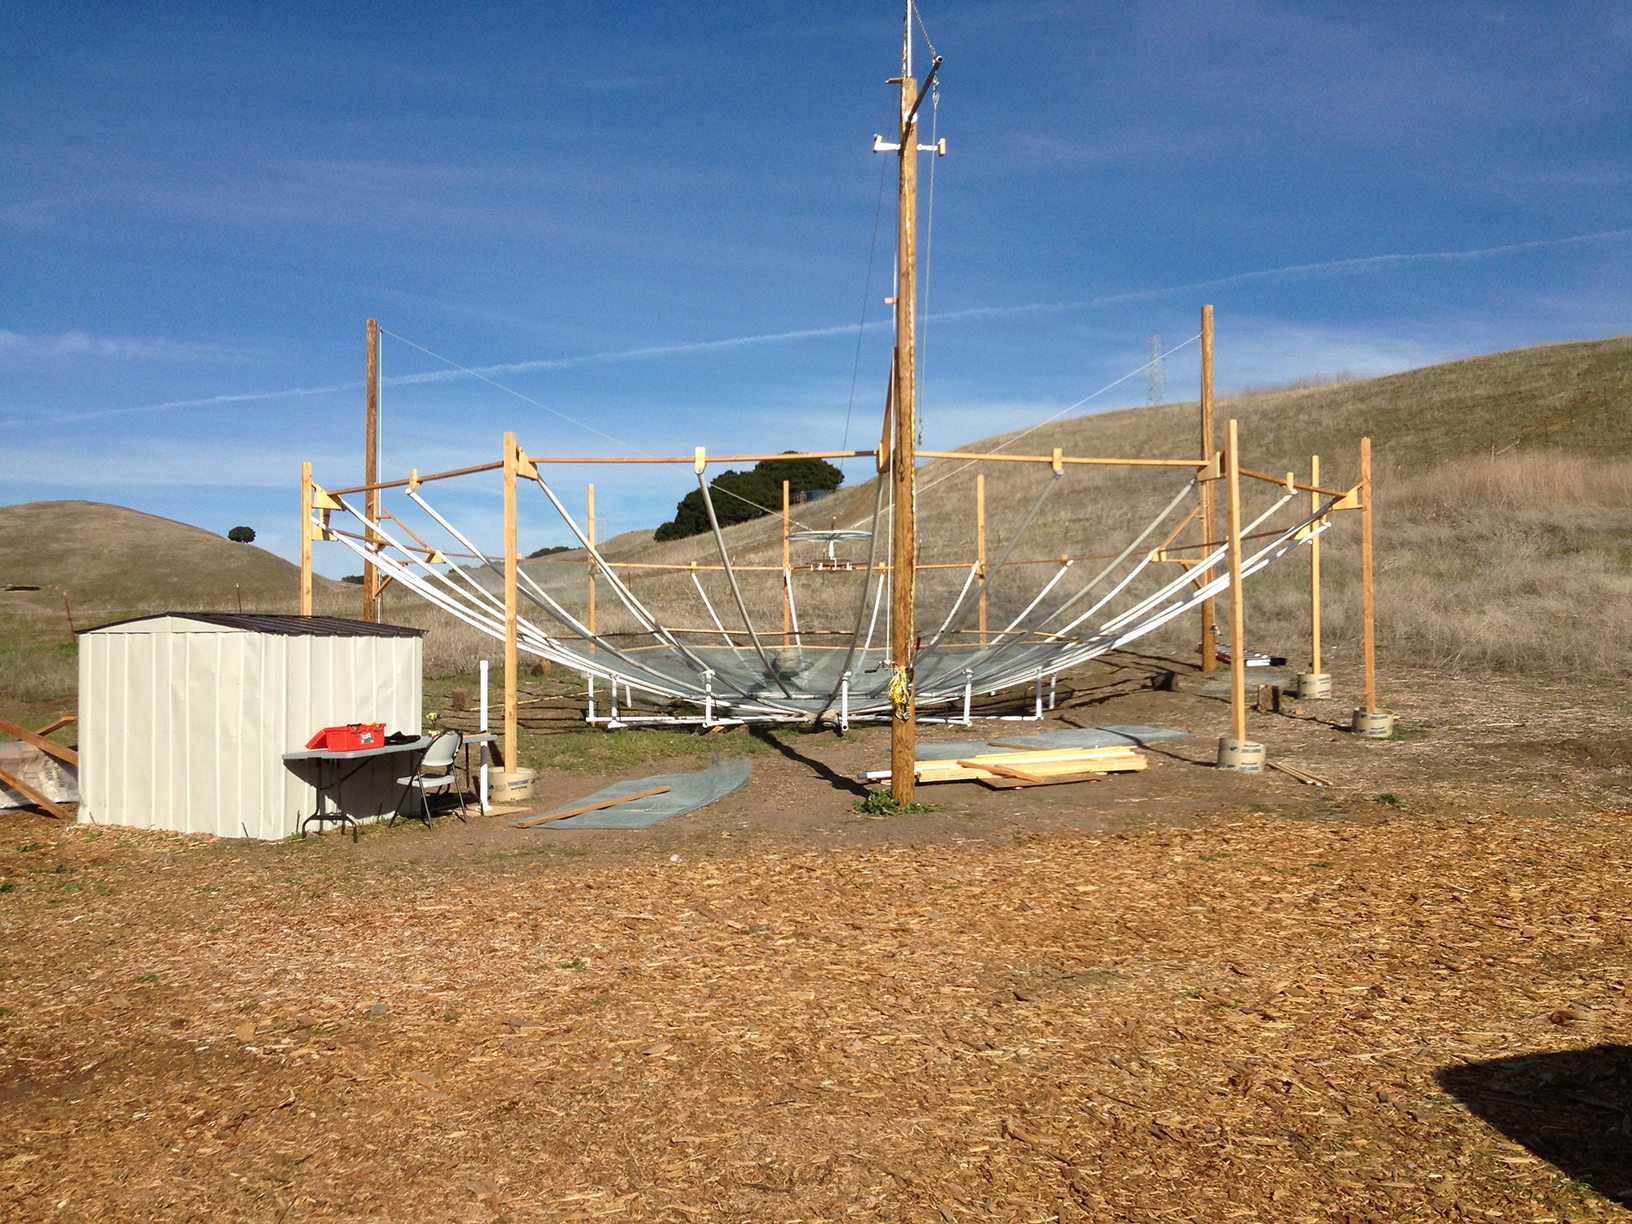
\includegraphics[width=0.46\textwidth]{plots/heracles.png}
	%\end{subfigure}
	%\quad
	%\begin{subfigure}[b]{0.46\textwidth}
		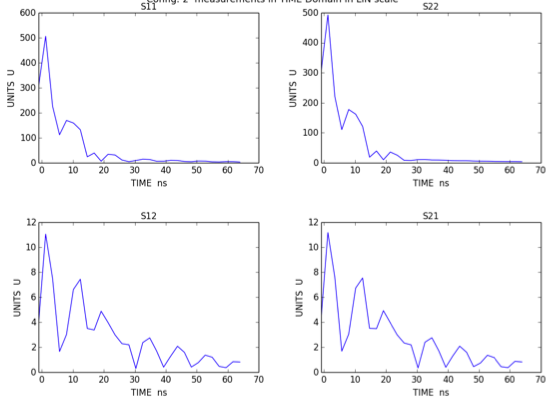
\includegraphics[width=0.46\textwidth]{plots/Engineering/heraclesNA.png}
	%\end{subfigure}
	\caption{Prototype antenna and initial results.
		Left: the existing construction prototype in California.
        Right: Initial reflection measurements from the prototype.}
	\label{fig:heracles}
\end{figure}

These additional prototypes will be important to finalize the specific construction techniques to be 
used in the final antenna construction contract in South Africa.

\vspace{-0.25in}
\subsection{Array Construction}
\vspace{-6pt}
Construction of HERA elements in the array consists of five primary steps: 
\begin{enumerate}[noitemsep,nolistsep]
\item site preparation and surveying 
\item pole installation by contracted labor with specialized utility pole equipment 
\item hub placement and height adjustment
\item remainder of construction of each element, following description above, using local labor 
\item moving the feeds and cables from the existing PAPER dipoles to new ground screens by project staff
\end{enumerate}

The contractors and immediate supervisors will be based in South Africa.  Supervision staff 
will be part of the extensive support infrastructure in place at the site to support South African SKA activities.
As mentioned above, the tall poles are shared amongst the antennas in the tight configuration.  
These are standard telephone/power 
utility poles and a great deal of  expertise and infrastructure exists to install these in remote settings.  
Figure \ref{fig:config_optics} (left panel) shows the antenna configuration, including the tall pole locations.
The right panel shows a cross-section of an element.

% AAARRGGHH!
\begin{figure}[h]
	\centering
	%\begin{subfigure}[b]{0.35\textwidth}
		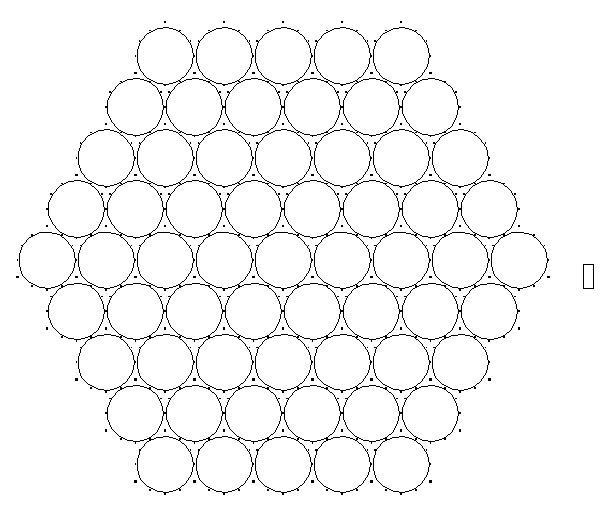
\includegraphics[width=0.35\textwidth]{plots/Engineering/hex_61.png} % XXX update this
	%	\label{fig:config}
	%\end{subfigure}
	%\quad
	%\begin{subfigure}[b]{0.6\textwidth}
		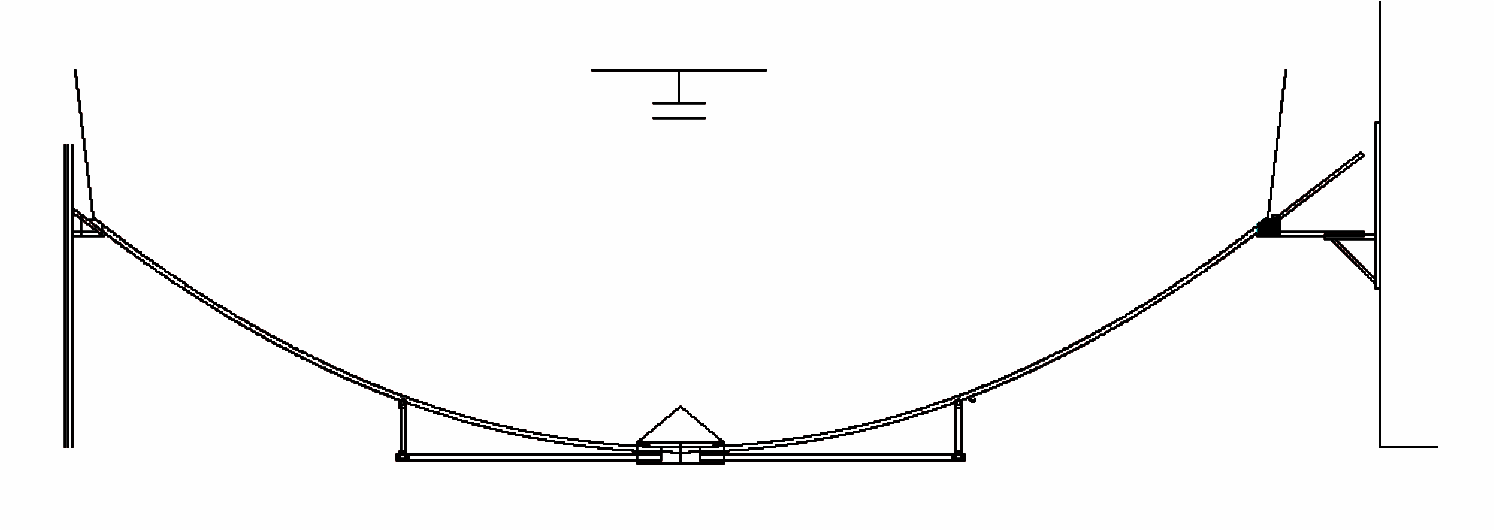
\includegraphics[width=0.6\textwidth]{plots/Engineering/optics.png}
		%\label{fig:optics}
	%\end{subfigure}
\caption{Left: the configuration of the 331-element array.  Note the rectangular container to scale on right.
		Right: a cross-section and optics of an element.}
	\label{fig:config_optics}
\end{figure}

Except for two custom metal assemblies, the remainder of the construction materials are standard wood, 
metal and PVC parts.  The two custom assemblies are simple small welded metal assemblies for the end of 
rim support pieces (quantity 12) and the feed and feed backplane (quantity 1).  The PVC and wood sub-assemblies 
will be constructed off-site where material and labor is readily accessible and shipped to site.  The 
construction of these sub-assemblies, pre-cut wood and PVC, and wire mesh pieces will be done on-site under 
contract.  Project staff will then move over the existing PAPER feeds and cables and commission the array.  

\vspace{-0.25in}
\subsection{Commissioning}
\vspace{-6pt}
Note that since all of the electronics are already deployed and working, commissioning will consist of verifying the existing performance but within the new electromagnetic environment presented by the new ground screens.  Below is
an explicit list of commissioning tasks:
\begin{itemize}[noitemsep,nolistsep]
\item equalization of signal levels and repairing of reflections and misbehaving signal paths due to cabling using auto-correlation data 
\item measure system temperature from raw level of auto-correlation data as it varies diurnally.
\item measure relative width of primary beam using source transits for XX and YY polarizations 
\item use established sky model from PAPER and correlation with known PAPER feeds to 
determine absolute gain as a function of direction for new dishes. 
\item use redundancy to solve for phase and gain calibration parameters, measure stability of parameters versus 
time 
\item detailed characterization of cross-coupling and reflections between antennas using cross-correlation data and imaging 
\item fold calibrated data on the basis of redundancy and multiple observing days to obtain a high-sensitivity delay spectrum capable of verifying absence of low-level reflections at higher delays. 
\end{itemize}

\subsection{Analysis and Science}

Beyond the construction and data-taking aspects of HERA, this proposal incorporates a full data analysis effort, culminating in the publication of a suite of science papers connecting observations to the theory of cosmic dawn.

\subsubsection{Calibration}

Building off the success of PAPER and MITEoR in such efforts, we will implement a real-time redundancy-based calibration pipeline.  The instantaneous calibration solutions provided by this pipeline allows one to quickly identify hardware misbehaviors, in addition to producing coarse real-time images.  The absolute calibration of these images will be fixed using a combination of self-calibration techniques and absolute-calibration baluns.  Increasingly detailed imaging efforts will then allow the development of empirical beam models (based on both sky models and octocopter signals) to complement electromagnetic simulations.  This is particularly important for characterizing the polarization response, which may affect estimates of polarization leakage.

Second, once data quality is assured, multi-day periods of data may be
binned in local sidereal time, and averaged. This intermediate
averaging scheme will also generate an accurate visibility-based sky
model for the instrument once calibration is applied.

\subsubsection{Foreground Modeling and Removal}
\label{sec:DataProducts}

A high dynamic range imaging pipeline based on the Fast Holographic Deconvolution (FHD; \citealt{sullivan_et_al2012}) pipeline of the MWA will be adapted for HERA.  The result will be sky maps with full Stokes information that can be used not only for better foreground suppression, but also as an interesting data product in itself.  We plan to perform detailed studies of the polarized sky, such as characterizing the distribution of rotation measures.  Updates to source catalogs and the Global Sky Model \citep{deoliveira2008} will provide reference sky models for both HERA and other low-frequency instruments. The goal will be to generate a model suitable for direct subtraction of foregrounds. 

% XXX need more data products here

\subsubsection{Power spectrum and related measurements}

In early power spectrum measurements, we will employ the conservative delay-spectrum approach to power spectrum estimation used in PAPER.  This visibility-based approach, when coupled with a foreground-avoidance strategy, will be sufficient for an unambiguous early detection of the $21~\textrm{cm}$ power spectrum should results from current-generation experiments prove marginal (see Figure \ref{fig:eor_pspec} and Table \ref{tab:signif}).  Further development plans will target the incorporation of optimal quadratic estimators \citep{liu_tegmark2011,dillon_et_al2013a} in both visibility and image spaces, incorporating a fully covariant description of the foreground wedge.  This will enable statistical foreground mitigation techniques in addition to those based on foreground modeling (for example, from FHD).  Finally, we plan to explore Bayesian techniques for power spectrum estimation, building on the considerable progress already made on Gibbs-sampling imaging for interferometers \cite{sutter_et_al2014}.  Any techniques developed should be equally applicable to measurements in both the reionization epoch and the Dark Ages.

To provide verification of our power spectrum constraints, we also plan to develop a simulator of the full HERA instruments, incorporating foregrounds and reionization models to output visibilities.

\subsubsection{HI Imaging}
Deep images will be summed to map HI emission (as described by Section \ref{sec:imaging_HI}) during reionization.   Foreground removal will follow the same basic plan as the power spectrum strategy.  Initially, residual images will be generated using the same conservatively foreground filtered and averaged data as input to an imager (e.g. FHD).  A subsequent, more sensitive method will use the image domain residuals generated by subtracting a foreground model.  Work on this method parallels the development of the precision foreground imaging and removal.

Sensitivity and significance of the images will be estimated by further developing the simulations shown in figure \ref{sec:imaging_HI}.  

%XXX need something here

%\subsubsection{Aspirations [move to facilities section?]}
%
%i. FFT correlator
%ii. other


\subsection{Schedule and Milestones} % 0.5 page
% De Boer

4 year proposal.
Cycle of development, testing, critical design review, deployment, commissioning, observation.
A more detailed scheduled is contained in the project management plan, but Table \ref{tab:scheduleSummary} gives an overview
of the milestones and deliverables.

\begin{table}[h]
\centering
\caption{Schedule Overview}
\label{tab:scheduleSummary}
\begin{tabular}{| p{1.5in} | p{1.5in} | p{1.5in} | p{1.5in} |}\hline
\textbf{Year 1}:  FY2015   &  \textbf{Year 2}:  FY2016  &  \textbf{Year 3}:  FY2017 & \textbf{Year 4}:  FY2018 \\ \hline
\raggedright{Infrastructure, prototyping and contract preparation.} &
\raggedright{Hardware commissioning and deep foreground survey.} &
\raggedright{HERA-127 observations:  detecting the rise and fall of reionization.} &
HERA-331 observations:  measuring the evolution of the first galaxies. \\ \hline  %It won't let me make this one raggedright!
\begin{itemize}[noitemsep,nolistsep,leftmargin=12pt]
\item Basic infrastructure
\item GB, SA prototypes
\item Design package
\item Polarization software
\end{itemize} &
\begin{itemize}[noitemsep,nolistsep,leftmargin=12pt]
\item HERA beam pattern
\item HERA-127
\item Delay-spectrum/FHD software
\item Analysis pipelines
\end{itemize} &
\begin{itemize}[noitemsep,nolistsep,leftmargin=12pt]
\item HERA-127 observations
\item Electronics upgrade
\item HERA-331
\item HERA-127 analysis
\end{itemize} &
\begin{itemize}[noitemsep,nolistsep,leftmargin=12pt]
\item HERA-331 observations
\item Cross-correlations
\item Cosmological simulations
\end{itemize} \\ \hline
\end{tabular}
\end{table}

% XXX
% need to discuss in a few sentences the
% relation to other experiments in the same time frame.


%\begin{itemize}[noitemsep,nolistsep]
%\item{Year 1:} Infrastructure, Prototyping, Contract Preparation (FY 2015).      
%\begin{itemize}[noitemsep,nolistsep]
%\item Install basic infrastructure (ground leveling, power, network connectivity) for new infrastructure
%\item Incorporate existing PAPER-128 antennas, correlator, and housing container.
%\item Install additional prototypes in Green Bank and test.
%\item Define final design package for element construction
%\item Start developing improved HERA baluns, receivers, feeds, nodes, and in-situ antenna calibration system.
%\item Continue delay-spectrum, FHD, and optimal estimator software development.
%\item Develop polarization capable software for beam/leakage studies.
%\end{itemize}
%\item{Year 2:} Hardware Commissioning and Deep Foreground Survey (FY 2016).  
%\begin{itemize}[noitemsep,nolistsep]
%\item Observations using PAPER antennas in an imaging configuration.
%\item Determine on-sky beam response of HERA antennas to facilitate future source subtraction efforts.
%\item Finalize site infrastructure (high-bandwidth optical network, surveying, trenching).
%\item Commission new feeds, receivers, nodes, and calibration systems in Green Bank and SA.
%\item Complete HERA-127 construction
%\item Initial delay-spectrum, FHD, and optimal estimator software ready for HERA 127 analysis.
%\item Full end-to-end simulations of analysis pipelines.
%\end{itemize}
%\item{Year 3:} HERA 127 and Detecting the Rise and Fall of Reionization (FY 2017).  
%\begin{itemize}[noitemsep,nolistsep]
%\item HERA 127 complete. Science observations begin using the PAPER correlator.
%\item Begin deployment of HERA 331. Install new node electronics and a 331-element, GPU-based correlator in the Karoo Array Processing Building (KAPB).
%\item Install new data storage infrastructure in the KAPB.
%\item Upgrade the UPenn analysis cluster.
%\item Finish construction of HERA 331
%\item Apply proven delay-spectrum analysis techniques to HERA 127 observations to constrain the timing and duration of reionization.
%\item Multi-pipeline analysis of HERA 127 observations to compare pipeline strengths/weaknesses.
%\end{itemize}
%\item{Year 4:} HERA 331 and Measuring the Evolution of the First Galaxies (FY 2018).           
%\begin{itemize}[noitemsep,nolistsep]
%\item HERA 331 complete. Begin science observations Oct. 2017.\item Begin multi-pipeline analysis of data to characterize the evolution of the power spectrum and determining properties of the first galaxies. 
%\item Continue analysis software development: optimize existing algorithms and develop imaging-based subtraction techniques for expanding the EoR window
%\item Create high-fidelity maps/data cubes of the HERA field for cross-correlation studies
%\item Cosmological simulations for extracting reionization physics from power spectrum measurements
%\end{itemize}
%\end{itemize}

\subsection{Assessment}

Point to Project Management Plan for details of milestones and design review criteria for each subsystem.
Each subsystem is tested prior to a critical design review that assesses the readiness of each subsystem.
Deployment and integration is coupled with commissioning activities that verify communication and control over defined interfaces.
Calibration 


%  ___                  _           ___                     _      
% | _ )_ _ ___  __ _ __| |___ _ _  |_ _|_ __  _ __  __ _ __| |_ ___
% | _ \ '_/ _ \/ _` / _` / -_) '_|  | || '  \| '_ \/ _` / _|  _(_-<
% |___/_| \___/\__,_\__,_\___|_|   |___|_|_|_| .__/\__,_\__|\__/__/
%                                            |_|        

\section{Broader Impacts} % 1 page
% Aguirre

% XXX The Broader Impacts need to be better developed.

%XXX Figure of students/interns

%A. pre and post-doctoral students
\subsection{Student Education}
%proposals must include, and will be evaluated on, a substantial component of
%student training and involvement of a diverse and inclusive workforce in
%instrumentation, facility development, or data management/analysis.

The HERA program will train new instrumentalists at the graduate and undergraduate levels, increase the
diversity of US graduate programs by engaging South African students and preparing them for admission to US degree programs, and make major data products available publicly as a benefit to the community.

Focus on UCB. 
Point to founding of CASPER at UCB.
Involving undergraduate, RAL intern, grad students, and postdocs, working alongside seasoned veteran engineers in a laboratory setting.
Recruiting of engineering students into science.
Focus on both development, testing, and documentation phases of instrument development.  
Involvement in design reviews.
Harnessing energy of young students, combining with the stability and discipline.
Synergy with Parsons' CAREER grant supporting pedagogical videos and other resources, integrated with relevant
research topics.

Through CASPER, via mail-lists, visiting students, workshops, dissemination of engineering expertise to a community broader
even than the set of students and engineers supported under this proposal.
Annual workshops.
Hosting visiting students (reference next section). Cite past cases: Manley, Landon, Zhang (Omniscope).
Mention specific success cases in progressing careers of instrumentalists: Parsons, Siemion, Ali, Hsyu, Leung, etc.

Although a critical core of instrument development and construction takes place at UC Berkeley, where it may be tightly
integrated and managed, each institution contributes necessary instrumentation, computing, monitor/control, data management, and
analysis software to the project.  
For these subsystems, students and postdocs take a leading role in development and testing.
Required participation in critical design reviews.
Involvement of students at all institutions in deployment, commissioning, and observing.


%B. South Africa connection
\subsection{South African Connection}
%i. professional development/exchanges

\subsubsection{Student Exchange}

We propose to broaden the scientific and technical impact of HERA by a program of student exchange between HERA and South African scientific collaborators.  This exchange is intended to be a mutually beneficial experience, with students on both sides being prepared to be world leaders in astronomy, and particularly in future work with next-generation 21 cm reionization experiments, and with the Square Kilometre Array (SKA).  Both scientific and engineering exchanges will be part of this program.  

Experience has shown that students benefit tremendously from peer mentoring and a sense of community, particularly when operating in a new cultural environment.  This is similar to the approach taken for South African students in their National Astrophysics and Space Science Programme (NASSP)
%; http://www.star.ac.za/) 
and also in US programs (e.g., the Posse Foundation).
%http://www.possefoundation.org/).  
Our student exchange program would pay special attention to bridging issues of scientific culture, allowing both groups to function at the highest possible level within their exchange community.  We anticipate that this program will prepare students on both sides to be able to productively apply for graduate, postdoctoral, and faculty positions in the exchange country, and to effectively apply for observing time on the SKA and NRAO facilities.  The net effect is an increase in the size and diversity of the talent pool.

SKA-SA has been consciously and actively prioritizing support to previously disadvantaged South Africans.  A deliberate focus is on addressing gender and race inequality in science and engineering at all levels, by prioritising support to black and women South Africans at undergraduate level, identifying non-traditional students, and guiding and supporting them into higher levels of research.  The level of financial support provided by SKA-SA at all levels of study and research ensure that the students do not have to concern themselves with finding employment immediately after graduating from a degree, a problem faced by many students who have obligations to contribute to their families’ income.

Specifically, we propose that each year of the grant, an exchange would be organized around a group of students (3 – 4) from each of the USA and RSA who would travel to a specific exchange institution to work on a related set of research problems over the course of a 3 month period (e.g., the northern summer).  These students would interact with both the host institution’s faculty and also the postdoctoral and graduate researchers there.  Budget allowance is made for the students' travel, lodging and meals.  For students in a Master’s program, this might represent their only exchange, and they would be mentored on application into PhD programs or engineering positions.  PhD candidates would participate in multiple exchanges, with the goal of establishing a sufficient scientific presence in their host country to apply to build post-graduate collaborations, apply for postdoctoral or permanent positions, and be in an excellent position to make good use of the host country’s radio astronomy facilities.  In order to vary the experience, each year would have a different host institution on each side, subject to the availability of mentors.  Building on past success with the CASPER program, the Berkeley cohort will be focused primarily on digital engineering.  

%ii. broader outreach in SA
\subsubsection{Broader Outreach in SA}

PAPER has an admirable history of enlisting interns from South African universities as part of major engineering deployments, with the work applied as practical training within their academic program.
Plans for incorporating outreach and education tours of SA universities as part of regular site visits.



%  ___                __ _ _      
% | _ ) ___ _ _  ___ / _(_) |_ ___
% | _ \/ -_) ' \/ -_)  _| |  _(_-<
% |___/\___|_||_\___|_| |_|\__/__/

\section{Benefits to the Astronomical Community}
%\subsection{Impacts for the Broader Astronomy Community}

%i. Data access: transients, SETI, ionosphere
The HERA measurements will be released to the community after an 18-month proprietary period and hosted on a public server at MIT (see Section \ref{sec:DataProducts}).  A large number of data products will be available.  Imaging products will include coarse real-time calibrated snapshot images in addition to high dynamic range survey maps from the FHD pipeline.  Calibrated, compressed, LST-binned visibilities will also be made public for re-analysis.  Higher cadence data sets will not be hosted publicly in a continuous fashion due to data transfer limitations, but will be available to any users upon request.

A number of derived data products will also be made accessible.  Source catalogs will be provided, and a Global Sky Model of diffuse foregrounds will be updated with new observations and released.  Foreground-subtracted data cubes of high-redshift $21\,\textrm{cm}$ intensity maps and the associated ionization field will be available for cross-correlation studies, as well as to provide context for high redshift optical and IR studies.

% ii. Cross correlation: CMBpol, CO/CII IM
%On the HERA timescale, a number of new observations will come online that would benefit from cross-comparison with the power spectra and images produced by HERA (see Section \ref{sec:CrossCorrelation}). For example, HERA will provide the large-scale reionization environment for pointed JWST or ALMA galaxy observations and can offer cross-correlations with  the WFIRST near-IR surveys \citep{lidz_et_al2009}.
 
CASPER.
Cite high rate of adoption of CASPER hardware in the community.
Delivering a next generation of signal processing platform.
Development of heterogeneous computing systems involving CPUs, GPUs, and FPGAs, including DSP libraries, data handling, and control software.
Sharing of LEDA GPU code \citep{clark_et_al2011} with PAPER's FPGA processors, data handling, and control software.
Continued support and development for the benefit of the radio astronomy instrumentation community.



%  ___                                
% / __|_  _ _ __  _ __  __ _ _ _ _  _ 
% \__ \ || | '  \| '  \/ _` | '_| || |
% |___/\_,_|_|_|_|_|_|_\__,_|_|  \_, |
%                                |__/ 

\section{Summary} % 0.5 pages
% Parsons

This HERA proposal follows the vision for 21~cm observations laid out in NWNH.
PAPER and the MWA have already succeeded in the primary task envisioned in
NWNH---characterizing the astrophysical foregrounds and developing the hardware
and analysis 
tools needed to suppress the contamination. The discovery and
characterization of the EoR Window and the development of precision foreground
mitigation techniques have shown that foregrounds can be suppressed to the current
thermal noise level (\S \ref{sec:Lessons}; \citealt{parsons_et_al2013}). While the MWA,
PAPER, and LOFAR are pushing hard to detect the EoR power spectrum, %budget constraints have
%dictated that 
a marginal detection is the best these instruments are likely to achieve.
HERA will both ensure a high significance detection of the \HI 21~cm 
signal as
well as provide powerful constraints on the rise and fall of reionization \citep{pober_et_al2014}, how
early stars and structure formed, and which physical processes dominated heating at the end of the
cosmic dark ages (Figures \ref{fig:x_i_vs_z} \& \ref{fig:eor_pspec}).

As envisioned in NWNH, the US EoR projects (PAPER, MWA, EDGES, MITEoR) have
pooled their expertise to develop the second generation HERA experiment. This
has created a collaborative team with a deep well of scientific
experience---the majority of papers on EoR observations are authored by members
of the HERA team. By leveraging this expertise, the HERA design is significantly
less expensive than envisioned in 
NWNH and has greater scientific reach.

The last few years have been remarkably productive---we
understand foreground systematics and are pushing 
existing
instruments to their thermal limits. We are now ready to build the HERA
instrument envisioned in NWNH and realize the scientific promise of 21~cm
cosmology.
Studying the formation of the first luminous structures 
and how they reionize the Universe is a primary driver for 
nearly all major astronomical facilities over the next decade.
Such studies include direct 
observations of stars, gas, dust, and AGN in the
first galaxies using the JWST, TMT, ALMA, and the JVLA. HERA is 
a unique and necessary element in this panchromatic arsenal, providing
providing the \emph{only} direct window onto the impact of these sources on 
their large-scale environments.


\clearpage
\setcounter{page}{1}
\thispagestyle{empty}
%\bibliographystyle{apj}
%\bibliographystyle{hapj}
\bibliographystyle{jponew}
%\bibliography{proj_description}
\bibliography{biblio}

\end{document}

